\documentclass[
	english,
	a4paper,
	fontsize=10pt,
	parskip=half,
	titlepage=true,
	DIV=12,
	final
]{book}
\usepackage[
    a4paper,
    bindingoffset=0.2in,
    centering,
    marginparwidth=2in,
    textwidth=16cm,
    marginparsep=2em,
    top=2cm,
    bottom=2.5cm,
    %showframe
]{geometry} 

\setlength{\parindent}{0em}
\setlength{\parskip}{1ex}


%==============================================================================%
% PACKAGES

% Standard text formatting
\usepackage[utf8]{inputenc}
\usepackage{babel}
\usepackage[T1]{fontenc}
\usepackage{lmodern}
\usepackage{microtype}
\usepackage{ragged2e}

\usepackage{csquotes}
\usepackage{xspace}

\usepackage[
	citecolor=black,
	colorlinks=true,
	linkcolor=black,
	anchorcolor=black,
	urlcolor=black,
	breaklinks=true
]{hyperref}

\usepackage{scrlayer-scrpage}
%\usepackage{setspace}

% Titles and text structure
\usepackage[explicit]{titlesec}
\usepackage{afterpage}
	\newcommand\blankpage{%
		\null
		\thispagestyle{empty}%
		\addtocounter{page}{-1}%
		\newpage}
\usepackage{epigraph}
	\setlength{\epigraphwidth}{.9\linewidth}
\usepackage[toc,page]{appendix}

% gfx
\usepackage{wrapfig}
\usepackage{graphicx}
\usepackage[bf]{caption}
	\captionsetup{
	format=plain,
	justification=raggedright,
	singlelinecheck=false
}
\usepackage{placeins}	% FloatBarrier.
\usepackage[table]{xcolor}
	\definecolor{titlebgdark}{RGB}{32,128,160}
	\definecolor{titlebglight}{RGB}{191,233,233}
	\definecolor{tabhighlight}{RGB}{230,240,255}
	\definecolor{grey}{RGB}{128,128,128}
	\definecolor{darkgrey}{RGB}{32,32,32}

\usepackage{tikz}
	\usetikzlibrary{positioning}
	\usetikzlibrary{matrix}
	\usetikzlibrary{shapes.geometric}
	\usetikzlibrary{backgrounds}
	\usetikzlibrary{calc}
	\usetikzlibrary{decorations.pathreplacing}
	\tikzstyle{every picture}+=[remember picture]
\usepackage{adjustbox}

\usepackage[most]{tcolorbox}

% tables
\usepackage{tabularx}
\usepackage{booktabs}
\usepackage{multicol}
\usepackage{multirow}
\usepackage{makecell}
\usepackage{color, colortbl}

% math
\usepackage{amsmath}
\usepackage{amssymb}
\usepackage{dsfont}
\usepackage[arrowdel]{physics}
\usepackage{mathtools}

\usepackage[newfloat]{minted}
	\usemintedstyle{friendly}
		
%==============================================================================%
% Headings definition

\titleformat{\chapter}[display]
  {\normalfont\huge\bfseries}
  {}
  {20pt}
  {%
    \begin{tcolorbox}[
      enhanced,
      colback=titlebgdark,
      boxrule=0.25cm,
      colframe=titlebglight,
      arc=0pt,
      outer arc=0pt,
      leftrule=0pt,
      rightrule=0pt,
      fontupper=\color{white}\sffamily\bfseries\huge,
      enlarge left by=-1in-\hoffset-\oddsidemargin, 
      enlarge right by=-\paperwidth+1in+\hoffset+\oddsidemargin+\textwidth,
      width=\paperwidth, 
      left=1in+\hoffset+\oddsidemargin, 
      right=\paperwidth-1in-\hoffset-\oddsidemargin-\textwidth,
      top=0.6cm, 
      bottom=0.6cm,
      overlay={
        \node[
          fill=titlebgdark,
          draw=titlebglight,
          line width=0.15cm,
          inner sep=0pt,
          text width=1.7cm,
          minimum height=1.7cm,
          align=center,
          font=\color{white}\sffamily\bfseries\fontsize{30}{36}\selectfont
        ] 
        (chapname)
        at ([xshift=-4cm]frame.north east)
        {\thechapter};
        \node[font=\small,anchor=south,inner sep=2pt] at (chapname.north)
        {\MakeUppercase\chaptertitlename};  
      } 
    ]
    #1
    \end{tcolorbox}%
  }
\titleformat{name=\chapter,numberless}[display]
  {\normalfont\huge\bfseries}
  {}
  {20pt}
  {%
    \begin{tcolorbox}[
      enhanced,
      colback=titlebgdark,
      boxrule=0.25cm,
      colframe=titlebglight,
      arc=0pt,
      outer arc=0pt,
      remember as=title,
      leftrule=0pt,
      rightrule=0pt,
      fontupper=\color{white}\sffamily\bfseries\huge,
      enlarge left by=-1in-\hoffset-\oddsidemargin, 
      enlarge right by=-\paperwidth+1in+\hoffset+\oddsidemargin+\textwidth,
      width=\paperwidth, 
      left=1in+\hoffset+\oddsidemargin, 
      right=\paperwidth-1in-\hoffset-\oddsidemargin-\textwidth,
      top=0.6cm, 
      bottom=0.6cm, 
    ]
    #1
    \end{tcolorbox}%
  }

%\titlespacing{<command>}{<left>}{<before-sep>}{<after-sep>}[<right>]  
\titlespacing*{\chapter}{0pt}{0pt}{40pt}
\titlespacing{\section}{0cm}{1.0cm}{0cm}
\titlespacing{\subsection}{0cm}{0.3cm}{0cm}

\usepackage{etoolbox}
\patchcmd{\chapter} % <cmd>
	{plain}         % <search>
	{empty}         % <replace>
	{}{}            % <success><failure>

%==============================================================================%
% tcolorboxes

\tcbsetforeverylayer{
	colback=cyan!10!white,
	colframe=titlebgdark,
	arc=0pt,
	outer arc=0pt,
	parbox=false
}
\newtcolorbox{defbox}[1][Your Title Here] {
	colback=cyan!10!white,
	colframe=titlebgdark,
	arc=0pt,
	outer arc=0pt,
	title=#1
}
\newtcolorbox{codebox}[1][Code] {
	colback=white,
	fontupper=\ttfamily ,
	colframe=blue!40!black,
	leftupper=7mm,
	title=#1,
	arc=0pt,
	outer arc=0pt
}
\newtcolorbox{cmdbox}[1][Command Line Interface] {
	colback=black,
	coltext=white,
	fontupper=\ttfamily ,
	colframe=blue!40!black,
	title=#1,
	arc=0pt,
	outer arc=0pt
}
\newtcolorbox{warnbox}[1][Attention] {
	colback=black!5!white,
	colframe=red!40!black,
	title=#1,
	arc=0pt,
	outer arc=0pt
}
\newtcolorbox{hintbox}[1][Hint] {
	colback=black!5!white,
	colframe=green!40!black,
	title=#1,
	arc=0pt,
	outer arc=0pt
}
\newtcolorbox{plusbox}[1][Advanced Content] {
	colback=yellow!5!white,
	colframe=yellow!90!red,
	coltitle=darkgrey,
	fontupper=\color{black},
	title=#1,
	arc=0pt,
	outer arc=0pt
}
\newenvironment{itembox}[1][] {
	\begin{tcolorbox}[title=#1,arc=0pt,outer arc=0pt]
	\begin{itemize}
}{
	\end{itemize}
	\end{tcolorbox}
}

%==============================================================================%
% GLOBAL MACROS

\newcommand{\myName}{Stefan Hartinger\xspace}
\newcommand{\myVersionTime}{June 2022}
\newcommand{\myTitle}{Programming in C\xspace}
\newcommand{\mySubtitle}{First Steps and Some Background\xspace}

\newcommand*{\ie}{i.\,e.\xspace}
\newcommand*{\eg}{e.\,g.\xspace}

\newcommand*{\tabcrlf}{\\ \hline}			% actually still allows for optional argument

\newcommand*{\smallfrac}  [2]{\ensuremath{{}^        {#1} \!/_        {#2}}}
\newcommand*{\smallfracrm}[2]{\ensuremath{{}^{\mathrm{#1}}\!/_{\mathrm{#2}}}}

\newcommand*{\thus}{\ensuremath{\rightarrow}\xspace}
\newcommand*{\Thus}{\ensuremath{\Rightarrow}\xspace}

\newcommand*{\citationneeded}{\href{https://xkcd.com/285/}{\color{blue}\textsuperscript{[citation needed]}}}

\newcommand{\inC}[1]{\mintinline{c}{#1}}

%==============================================================================%
% GLOBAL PARAMTERS

\title{\myTitle}
%\subtitle{\mySubtitle}
\author{\myName}
\date{\today}

% header, footer
\clearpairofpagestyles
	\cfoot
		[\pagemark]
		{\pagemark}
	\ohead
		[]
		{}
\pagestyle{scrheadings}

%==============================================================================%
% THE REAL STUFF
%
\begin{document}
	\begin{titlepage}
		\centering
		\makeatletter 		% activate some weird special mode that enables the use of \@title and other macros

		{\phantom{x}}
		
		\vspace{6\tabcolsep}
		\Huge \textsc{\@title}

		\vspace{6\tabcolsep}
		\LARGE \textsc{\mySubtitle}

		\vspace{6\tabcolsep}
		\large
		State \@date\\
		
		\vspace{7\tabcolsep}
		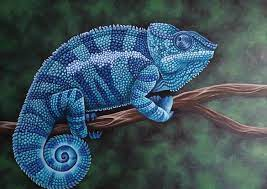
\includegraphics[width=.5\paperwidth]{./gfx/chameleon-dummy}
		%TODO replace by free/owned art; this one is from https://bluethumb.com.au/erin-hale/Artwork/the-chameleon-0 and costs USD 75...

		\vspace{6\tabcolsep}
		\large
		Blue Chameleon Coding \\
		
		\makeatother			% deactivate special mode for \@title, etc.
	\end{titlepage}

	{
		\pagestyle{empty}
		%\renewcommand*{\chapterpagestyle}{empty}

		\chapter*{Preface}
We shall start this course with realizing and internalizing a deep and profound truth that will follow us through our coding life and have an important impact on all our projects:

\begin{defbox}[Our Mantra]
\begin{center}
\begin{Huge}
	\emph{Computers are friggin stupid.}
\end{Huge}
\end{center}
\end{defbox}

In principle, this is well and good. If this statement would not hold, we'd have a really hard time making computers do the tasks that are too tedious for us. However, anyone who has ever tried to delegate a part of their chores to a less gifted contemporary knows how \emph{on point} the instructions for their coeval have to be. For computers, this is even only more so. In the tutorials, I've often heard the participants say things like \emph{I thought, the computer would understand that ...}, which I like to acquit with \emph{You think -- the computer does not.}

In this course, I want to guide you through both, the concepts according to which a computer works and the thought processes that you as a programmer should devellop to translate your real life goals into code. In particular, we will be learning the specifics of the programming language C. This language which first appeared in ancient times\footnote{\ie in 1972} has been expanded upon ever since and influenced virtually all modern languages such as C++, C\#, Java, Python, Rust, Go, Perl, Julia, ... You may think of this course as a general introduction to programming. If you ever get to learn another programming language, you will recognize most if not all the concepts discussed here.

This course is aimed at beginners. We will cover all relevant concepts from ground up. I try to keep things interesting while guiding you through the technical details; unfortunately, there are a bunch of them. That means I'll have to ask you to be patient. It will take us a while before we can do anything \emph{interesting} with our programs. However I firmly believe that being able to do things \emph{right} is more rewarding that being able to do things \emph{quickly}\footnote{at least if you can have only either of them.}. To make sure you understand correctly, I'll be providing lots of examples.

While I'll do my best to explain what works how and why, there's no way around doing exercises on your own. I will provide a number of quizz questions at the end of each chapter that are designed to solidify and deepen your understanding of code. Of course, you'll also find solutions in the appendix. Still, I want to encourage you to do your own experiments, be it small code snippets to try your intuition or exercises from external sources. In the end, coding is a skill you can only properly learn by doing.

I should also make clear at the very beginning that programming (in any language) means \emph{applied maths}. While you do not need to have majored maths in university, neither should you have an aversion against tinkering with formulae anf formal logic. A machine that was built to \emph{compute} can only be told what to do using the tools provided by maths.

Note also that this is an introductory course, not a complete reference of all aspects of the C programming language. As a such, I recommend the website \url{cppreference.com}, which does a good job listing all features and expected behaviours. In fact, since I regard this website an essential tool in programming, a short chapter will be dedicated to how to find your way in that encyclopedia.

To go through this course, you will need a current installation of the \emph{Gnu Compiler Collection} (GCC) as well as a simple code editor on your machine. You should find a guide for how to do so on the website where you found this book, as well as alternative options. Further, you should be (superficially) familiar with using the console for invoking programs. While there are other ways of compiling code, I will show exclusively how to do so from the command line. The reason behind this is that I feel in no way capable of treating the myriad of IDEs\footnote{\emph{Integrated Development Environment}; graphical programs that help with writing code.} available ot there, nor the differences that come with the versions written for different operating systems. The somewhat antiquated command line interface, on the other hand, is way more uniform between various machines. Last but not least, you can derive the correct handling of your IDE from understanding the command line; an IDE is only a \emph{frontend} to the command line interface, \ie it will generate the same commands that I shall show you here.

Since this approach means we are dealing with two different environments -- the command line and our C code -- it is only reasonable to reflect this fact graphically in this book. In- and Output on the command line will be rendered in black boxes like the following:
\begin{cmdbox}[Command Line Interface]
\texttt{{\color{green}blue-chameleon@blue-chameleon-HP-250-G8-Notebook-PC}:{\color{blue!80!white}\textasciitilde}\$ cd Codes} \\
\texttt{{\color{green}blue-chameleon@blue-chameleon-HP-250-G8-Notebook-PC}:{\color{blue!80!white}\textasciitilde\textbackslash Codes}\$}
\end{cmdbox}

More often than not, the preface to the command line interface (the green and blue text) will be omitted, and only the commands themselves as well as their output are presented. To distinguish between commands and output, the former will be prefaced with a Dollar sign (\texttt{\$}):

\begin{cmdbox}[Command Line Interface]
\texttt{\$ echo hello world} \\
\texttt{hello world}
\end{cmdbox}

C-Code, on the other hand, will be rendered in white boxes with \emph{syntax highlighted}\footnote{to make code easier readable for humans, it is custom to render the various parts in different colours. Syntax highlighting means applying these rules for colouring.} code together with line numbers:
\begin{codebox}[helloworld.c]
\begin{minted}[linenos]{c}
#include <stdio.h>

int main () {
    printf("hello world\n");
}
\end{minted}
\end{codebox}

Where relevant, I will also provide the output generated by a program after compiling and executing it. The invocation of the compiler and the compiled program itself will be discussed in the first chapter and omitted thereafter, unless something \enquote{non-standard} is going on.

A picture says more than a thousand words. Where possible, I will provide sketches to illustrate the key concepts of the current discussion. To make them even easier to find when skimming through the book, these schematics are highlighted in a sky blue box. These sketches will be enumerated and listed in the list of figures at the very end of this book. The same type of boxes is used at the end of each chapter to summarize the main takeaways.

\begin{defbox}[Path to Success]
\begin{center}
\begin{tikzpicture}
  [
    cell/.style={text width=80mm,
      text height=4mm, draw=black, inner sep=1mm},
    ld/.style={draw=black,shorten >=2pt,->}
  ]
  \node (c1) at (0,9.5) [cell] {Read and understand each chapter of this book};
  \node (c2) at (0,7.7) [cell] {Do the exercises at the end of each chapter before advancing};
  \node (c3) at (0,5.4) [cell] {Write some own sample codes and have fun while coding};
  \node (c4) at (0,3.6) [cell] {Start a bigger project after you finish this course};
  \node (c5) at (0,1.8) [cell] {Analyze which parts gave you trouble and rework them};
  \node (c6) at (0,0.0) [cell] {Learn from others};

  \draw [ld] (c1.south) -> (c2.north);
  \draw [ld] (c2.south) -> (c3.north);
  \draw [ld] (c3.south) -> (c4.north);
  \draw [ld] (c4.south) -> (c5.north);
  \draw [ld] (c5.south) -> (c6.north);
\end{tikzpicture}
\end{center}
\end{defbox}

Some text will be set off the principal text in a box with a grean headline. The content of these boxes is a tangent to what the full text tries to explain and will often contain good pieces of advice or clarifications. You should see them as part of the continuous text that is highlighted to easier find it later on.

\begin{hintbox}[List of Terms]
This book probably will introduce a lot of new concepts to you. If you've forgotten what a certain term means or where to find it, you can look at appendix A. There you'll find an alphabetical list of the concepts and terms introduced in this book.
\end{hintbox}

\emph{errare humanum est} -- and you presumably are one. Don't worry, I've got you covered. To warn you about situations most beginners (and sometimes even professionals) struggle with, I put boxes with red headlines that show you situations you should avoid, or code that contains a non-obvious error.

\begin{warnbox}[Do not learn all of this by heart]
A good programmer does not necessarily know \emph{all} the details shown in this book. It is sufficient to broadly know about concepts and look up the details when the need arises. Don't bother yourself with memorizing tables that you can look up online or in this book whenever you need to. You will automatically retain the truly important bits simply by repeatedly applying them. Rather, spend your energy on understanding, and doing experiments on your own!
\end{warnbox}

Some of the content is certainly interesting, but maybe less so for absolute beginners; at the very least, those sections are not essential for every day coding. Depending on your level and time restraints, you may want to do a deep dive or cut to the chase. To faciliate this, more advanced content is highlighted in a similar manner:
\begin{plusbox}
In assembly, the hello world program expands to
\begin{codebox}[helloworld.s]
\begin{minted}[linenos]{asm}
        .file   "helloworld.c"
        .text
        .section        .rodata.str1.1,"aMS",@progbits,1
.LC0:
        .string "hello world\n"
        .section        .text.startup,"ax",@progbits
        .p2align 4
        .globl  main
        .type   main, @function
main:
.LFB12:
        .cfi_startproc
        endbr64
        subq    $8, %rsp
        .cfi_def_cfa_offset 16
        leaq    .LC0(%rip), %rsi
        movl    $1, %edi
        xorl    %eax, %eax
        call    __printf_chk@PLT
        xorl    %eax, %eax
        addq    $8, %rsp
        .cfi_def_cfa_offset 8
        ret
        .cfi_endproc
.LFE12:
        ...
\end{minted}
%$
\end{codebox}
\end{plusbox}

This book is based on a university level course for which I was responsible from 2018 through 2022. The experience with different kinds of students and their learning styles have informed the course design in numerous ways. However, time constraints have always curbed my ambitions, and I'm thrilled to expand on my prior work. Ultimatively, of course, this is a piece of human work, and therefore likely to be flawed. I put a lot of effort into the totality of this project, but I can almost guarantee you that you can find at least some minor mistakes. If you do so, or have any questions or remarks on the provided material, feel free to contact me: \url{bluechameleoncoding@gmx.net}

Without further ado, let's start coding!
\begin{flushright}
\myName, \myVersionTime
\end{flushright}
		\blankpage
		\pagestyle{empty}
		\tableofcontents

		\clearpage
	}

	\setcounter{page}{1}
	
	\chapter{How does a computer work?}
\epigraph{The good news about computers is that they do what you tell them to do. The bad news is that they do what you tell them to do.}{Ted Nelson}

In the general public, it is well known that computers effectively know only two states -- current flows or does not. These \emph{bits} of information are commonly represented by the digits 1 and 0. But how can these elementary states be assembled into complex programs?

\section{Binary Representation of Numbers}
Before we get to understand how, internally, \emph{programs} look like, let us first have a look at \emph{numbers}, ...

\subsection{Binary Representation of Positive Integers} \label{sec:BinaryNumbers}
... and more simply, positive integers. For that, let us start in the familiar decimal system, and look at a random number, say $1725$:

\begin{defbox}[Decomposition of a decimal integer]
\begin{center}
\begin{tikzpicture}[
  flow/.style={draw=black,->,shorten >=2pt}
]
  \node (s3) at (0, 2.3) {\tiny 3};
  \node (s2) at (1, 2.3) {\tiny 2};
  \node (s1) at (2, 2.3) {\tiny 1};
  \node (s0) at (3, 2.3) {\tiny 0};

  \node (n3) at (0, 2) {1};
  \node (n2) at (1, 2) {7};
  \node (n1) at (2, 2) {2};
  \node (n0) at (3, 2) {5};

  \node (e3) at (4.5, 0.0) {$1 \times 10^3 = 1000$};
  \node (e2) at (4.5, 0.5) {$7 \times 10^2 = ~700$};
  \node (e1) at (4.5, 1.0) {$2 \times 10^1 = ~~20$};
  \node (e0) at (4.5, 1.5) {$5 \times 10^0 = ~~~5$};

  \draw[flow] (n3.south) |- (e3.west);
  \draw[flow] (n2.south) |- (e2.west);
  \draw[flow] (n1.south) |- (e1.west);
  \draw[flow] (n0.south) |- (e0.west);
  
  \node (l0) at (3.0, -0.3) {};
  \node (l1) at (6.0, -0.3) {};
  \draw[double] (l0) -- (l1);
  
  \node (re) at (5.3, -0.6) {$1725$};
\end{tikzpicture}
\end{center}
\end{defbox}

We start by enumerating the digits of our number $1725$ \emph{from the right} and \emph{starting with $0$}; indices will be called \emph{exponents}, and the reason for that will become clear in a second. The contribution of each digit to the whole number ist given by the product of the digit's value and the power of base $10$ to the exponent. Summing up all individual contributions restores the number from which we started -- $1725$.

This may seem a tedious and very technical exercise in a concept we've known since primary school. The benefit of these considerations is the realization that the same concept can be applied to other \emph{base systems} as well: if we don't have ten digits (as in our \emph{decimal system}), but only two (\ie if we use the \emph{binary system}), then all we have to do is to replace the base $10$ with base $2$ and follow the same rules. For example, we find:

\begin{defbox}[Decomposition of a binary integer]
\begin{center}
\begin{tikzpicture}[
  flow/.style={draw=black,->,shorten >=2pt}
]
  \node (s10) at (00, 0.8) {\tiny 10};
  \node (s09) at (01, 0.8) {\tiny 9};
  \node (s08) at (02, 0.8) {\tiny 8};
  \node (s07) at (03, 0.8) {\tiny 7};
  \node (s06) at (04, 0.8) {\tiny 6};
  \node (s05) at (05, 0.8) {\tiny 5};
  \node (s04) at (06, 0.8) {\tiny 4};
  \node (s03) at (07, 0.8) {\tiny 3};
  \node (s02) at (08, 0.8) {\tiny 2};
  \node (s01) at (09, 0.8) {\tiny 1};
  \node (s00) at (10, 0.8) {\tiny 0};

  \node (n10) at (00, 0.5) {1};
  \node (n09) at (01, 0.5) {1};
  \node (n08) at (02, 0.5) {0};
  \node (n07) at (03, 0.5) {1};
  \node (n06) at (04, 0.5) {0};
  \node (n05) at (05, 0.5) {1};
  \node (n04) at (06, 0.5) {1};
  \node (n03) at (07, 0.5) {1};
  \node (n02) at (08, 0.5) {1};
  \node (n01) at (09, 0.5) {0};
  \node (n00) at (10, 0.5) {1};

  \node (e00) at (12.5, -0.0) {$1 \times 2^{0} ~= ~~~~1$};
  \node (e01) at (12.5, -0.5) {$0 \times 2^{1} ~= ~~~~0$};
  \node (e02) at (12.5, -1.0) {$1 \times 2^{2} ~= ~~~~4$};
  \node (e03) at (12.5, -1.5) {$1 \times 2^{3} ~= ~~~~8$};
  \node (e04) at (12.5, -2.0) {$1 \times 2^{4} ~= ~~~16$};
  \node (e05) at (12.5, -2.5) {$1 \times 2^{5} ~= ~~~32$};
  \node (e06) at (12.5, -3.0) {$0 \times 2^{6} ~= ~~~~0$};
  \node (e07) at (12.5, -3.5) {$1 \times 2^{7} ~=  ~128$};
  \node (e08) at (12.5, -4.0) {$0 \times 2^{8} ~= ~~~~0$};
  \node (e09) at (12.5, -4.5) {$1 \times 2^{9} ~=  ~512$};
  \node (e10) at (12.5, -5.0) {$1 \times 2^{10} =  1024$};
  
  \draw[flow] (n10.south) |- (e10.west);
  \draw[flow] (n09.south) |- (e09.west);
  \draw[flow] (n08.south) |- (e08.west);
  \draw[flow] (n07.south) |- (e07.west);
  \draw[flow] (n06.south) |- (e06.west);
  \draw[flow] (n05.south) |- (e05.west);
  \draw[flow] (n04.south) |- (e04.west);
  \draw[flow] (n03.south) |- (e03.west);
  \draw[flow] (n02.south) |- (e02.west);
  \draw[flow] (n01.south) |- (e01.west);
  \draw[flow] (n00.south) |- (e00.west);
  
  \node (l0) at (11.0, -5.3) {};
  \node (l1) at (14.0, -5.3) {};
  \draw[double] (l0) -- (l1);
  
  \node (re) at (13.3, -5.6) {$1725$};
\end{tikzpicture}
\end{center}
\captionof{figure}{Decomposition of a binary integer}
\end{defbox}

\emph{Any} positive integer can be transformed in that manner. Note that with $N$ bits, you can form $2^N$ integers, ranging from $0$ to $2^N - 1$.

\subsection{Negative Numbers in Binary}
There are more numbers than positive integers\citationneeded. How do we expand our existing system onto \emph{negative} numbers?

In the world we are used to, there is no problem adding more characters to the set we represent numbers with. In a computer, this would be much more difficult. We somehow have to do with ones and zeros only. A way to solve this is to \emph{limit the number of digits} and select one special digit that is exempt from our interpretation scheme but will serve as a \emph{sign bit}.

\begin{defbox}[Example: Three bit integer with sign bit]
Assume, we use three digits to represent a signed number. Then, the following bitpatterns correspond to these decimal integers:

\begin{center}
\begin{tabular}{cc|cc}
Binary & Decimal & Binary & Decimal \tabcrlf
000 & 0 & 100 & -0 \\
001 & 1 & 101 & -1 \\
010 & 2 & 110 & -2 \\
011 & 3 & 111 & -3
\end{tabular}
\end{center}

The first two bits (bit exponents 0 and 1) are interpreted as before. The \emph{highest order bit} (exponent 2) encodes the sign -- 0 for positive values, 1 for negative ones.
\end{defbox}

While this method fulfils its purpose, it has one glaring weakness: There are \emph{two} representations of the value $0$! This is a problem, since as a human we expect $0 = -0$ to hold; the computer, however, only sees different bitpatterns and therefore declares $0 \neq -0$!

To mitigate this, the so called \emph{two's complement} is employed: the sign bit gets a double role: when computing each digit's contribution, the sign bit is included in the interpretation scheme discussed before, but as a negative value:

\begin{defbox}[Example: Three bit integer with two's complement]
Again, we use three digits to represent a signed number. Then, the following bitpatterns correspond to these decimal integers:

\begin{center}
\begin{tabular}{cc|cc}
Binary & Decimal & Binary & Decimal \tabcrlf
000 & 0 & 100 & -4 \\
001 & 1 & 101 & -3 \\
010 & 2 & 110 & -2 \\
011 & 3 & 111 & -1
\end{tabular}
\end{center}

The first two bits (bit exponents 0 and 1) are interpreted as usual. The \emph{highest order bit} (exponent 2) gives a value of ${\color{blue}-}2^2 = -4$.
\end{defbox}

\begin{warnbox}[Everything is up for interpretation!]
As you see, the same bitbpattern can be interpreted in numerous ways! There is nothing inherent to the sequence of ones and zeros that could tell whether we are dealing with an unsigned or signed integer. As we will later see, this ambiguity also holds for floating point numbers, texts, programs, images, ...

Information in isolation is nigh-worthless. To do anything useful with it, we need some context that provides the way of interpretation for the given information. We will see later on how this is realized in the C programming language.
\end{warnbox}

\subsection{Byte Sized Chunks}
In the human world, we can (in principle) use an arbitrary number of digits to write down any number we fancy. While the binary system does allow the same degree of freedom, computers are more restrictive. Any piece of information will always be composed of an integer multiple of eight bits. We say, information always comes in units of \emph{bytes}.

Several bytes can be joint to form a bigger compound. That is, you can form a (potentially) bigger number out of two bytes. \enquote{Unused} bits will be padded with zeros. For example, the number $15$ could in principle be written as $1111_2$ (in which the index $2$ signifies that this is a binary number.) Since we have to use at least eight bits, in a computer it would be stored as the bitpattern \texttt{00001111}.

\begin{warnbox}[No obvious end]
Again, there is no inherent \enquote{end} of a number. A randomly picked byte from memory could equally well be the start, middle or end of a multi-byte number, or of course a stand-alone one-byte representation of a number. To know which is which, some context is needed which we will have to specify explicitly in our programs.
\end{warnbox}

\section{Binary Representation of Real Numbers}
Real numbers -- numbers with a decimal part, or \enquote{comma values} -- play an important our daily lives. Luckily, computers can handle them as well; of course, this means that there is a way to translate them into binary, as well. The most simple way of doing so would be to specify a fixed position where to insert the decimal point. While this works in principle, it has prooven too inflexible for most real life applications. Instead, a devious scheme to implement \emph{floating point numbers} has been devised. This scheme comes at the cost of introducing a small but sometimes noticeable \emph{rounding error} in each operation that involves such a floating point number.

In this course, we won't be handling floating point numbers a lot; still, it might be interesting for you to better understand how decimal numbers are stored in a binary machine. This is especially helpful when you do scientific simulations and need to minimize rounding errors.

\begin{plusbox}[Representation of real numbers as floating point numbers]
We can follow the same tracks as before when decomposing real numbers: we enumerate all digits of a base ten number, \emph{relative to the position of the decimal point}:
\vspace{\parskip}

\begin{defbox}[Decomposition of a decimal real number]
\begin{center}
\begin{tikzpicture}[
  flow/.style={draw=black,->,shorten >=2pt}
]
  \node (s3) at (0, 2.3) {\tiny 1};
  \node (s2) at (1, 2.3) {\tiny 0};
  \node (s1) at (2, 2.3) {\tiny -1};
  \node (s0) at (3, 2.3) {\tiny -2};

  \node (n3) at (0, 2) {1};
  \node (n2) at (1, 2) {7};
  \node (nd) at (1.5, 2) {\phantom{0}.};
  \node (n1) at (2, 2) {2};
  \node (n0) at (3, 2) {5};

  \node (e3) at (5.0, 0.0) {$1 ~\times$};
  \node (e2) at (5.0, 0.5) {$7 ~\times$};
  \node (e1) at (5.0, 1.0) {$2 ~\times$};
  \node (e0) at (5.0, 1.5) {$5 ~\times$};
  
  \node (f3) at (5.7, 0.0) {$10^1   $};
  \node (f2) at (5.7, 0.5) {$10^0   $};
  \node (f1) at (5.7, 1.0) {$10^{-1}$};
  \node (f0) at (5.7, 1.5) {$10^{-2}$};
  
  \node (g3) at (7.0, 0.0) {$= 10.00$};
  \node (g2) at (7.0, 0.5) {$= ~7.00$};
  \node (g1) at (7.0, 1.0) {$= ~0.20$};
  \node (g0) at (7.0, 1.5) {$= ~0.05$};

  \draw[flow] (n3.south) |- (e3.west);
  \draw[flow] (n2.south) |- (e2.west);
  \draw[flow] (n1.south) |- (e1.west);
  \draw[flow] (n0.south) |- (e0.west);
  
  \node (l0) at (4.5, -0.3) {};
  \node (l1) at (8.0, -0.3) {};
  \draw[double] (l0) -- (l1);
  
  \node (re) at (7.2, -0.6) {$17.25$};
\end{tikzpicture}
\end{center}
\end{defbox}

The same can be done in binary, again, assuming we have some means of encoding the position of the decimal point (e.g. by fixing the position in the binary representation where it is inserted). Doing so, the decimal number $0.5$ becomes $0.1_2$, the number $0.25$ becomes $0.01_2$ and so forth.

Like in the decimal system, there are numbers that are \enquote{problematic} to write down. Think of the fraction \smallfrac{1}{3} $\approx 0.333...$: you need an infinite number of digits to represent this number in the decimal system. To provide some mathematical insight: this happens whenever in the fractional representation of a number ($\smallfrac{p}{q}$), the denominator has prime factors other than those of ten, \ie other prime factors than 2 and 5.

In the binary system, the base has only one prime factor; hence, such \enquote{problematic} numbers are much more common. As in the decimal system, one simply accepts a little imperfection and works with a rounded number. So, instead of storing the infinite number of digits needed to represent $0.1$ in binary, one simply works with $0.1 \approx 0.0001100110011001101_2$.

You see that a significant number of binary digits is necessary to store the fractional part of a number with acceptable precision. This becomes worse when dealing with very small numbers.

In science, both very small and very large numbers are written down in \emph{scientific notation}: instead of writing $0.025$, one would put $2.5 \times 10^{-2}$ on the paper. This seems tedious for numbers close to 1, but very small numbers like the gravitational constant ($G \approx 6.67430 \times 10^{-11} = 0.0000000000667430$) become \emph{much nicer} to handle this way.
\end{plusbox}
%
\begin{plusbox}[]
We can do the same in binary: instead of storing the entire information in a singular number, we split it into a \emph{mantissa} ($6.67430$) and an \emph{exponent} part ($-11$) to the benefit of having a way more compact format for our data. Adding a sign bit to the recipe we get a number format that works well for a large range of numbers and uses the available precision as well as possible.

One consequence of this is that larger numbers implicitly are represented with less precision:

Back in the decimal system, think of the mantissa as holding a fixed number of decimal places. Then the uncertainty of this value is given by the exponent. The representation of $2.5 \times 10^{-2}$ could mean anything between $0.0245$ and $0.0254\overline{9}$ -- an uncertainty range of $0.001$. Given the same mantissa but a different exponent, the value $2.5 \times 10^{1}$ covers everything between $24.5$ and $25.4\overline{9}$, an uncertainty range of $1$.

While this rarely causes trouble when \emph{storing} numbers (it is rarely important whether a number is 9289347981238903 or 9289347981238904), problems arise when doing math with numbers of different orders of magnitude.

For example, let's add the numbers $1$ and $0.00001$. Storing them in scientific format with a mantissa lenght of four, they can be represented with perfect precision as $1.000 \times 10^{0}$ and $1.000 \times 10^{-5}$. Let's also assume this is the maximum storage place we want to allot per number. Any number that takes more space than that will be rounded to the next number representable with four mantissa digits. For example, the value $19937$ will be stored as $1.994 \times 10^{4}$.

Now, adding $1$ and $0.00001$ together gives $1.00001 = 1.00001 \times 10^{0}$, but would require six mantissa digits -- too much for our limited storage. Hence, the result gets rounded to $1.000 \times 10^{0}$. In other words, we have the \emph{mathematically incorrect} result that $1 + 0.00001 = 1$.

Getting around this problem is non-trivial. Of course, one can always use more mantissa bits (\enquote{more precision}); however, this comes at the cost of higher memory and computation time demand. Designing algorithms with the mechanics behind floating point numbers in mind and thereby minimizing the rounding errors if often the more apt way of dealing with this issue. In this course, we will not focus on this aspect of programming; be aware, though, that it exists.
\end{plusbox}

\section{Binary Representation of Non-Number Information}
Even though the name \emph{computer} already gives away, that these machines are best used for crunching numbers, we also want to (need to) handle information other than pure numbers. To put non-number data into binary memory, again some interpretation scheme has to be applied.

\subsection{Text in Memory}
There are different \emph{encodings} for textual information; all of them are based on the same principle: one can build a one-to-one correspondence between numbers and letters\footnote{or, more general, characters. Technically, \emph{letters} only describes the symbols \emph{a}...\emph{z} and \emph{A}...\emph{Z}, or their counterparts in the various other writing systems. But there's also punctuation, digits and other non-letter constituents of writing systems like line breaks, whitespaces or tabulators.}. We can enumerate all characters of a writing system and use the numbers to stand in for the textual information. For that, we only need to agree on a standard, \ie a ruleset that tells us which character is encoded by which number.

One of the oldest such encoding that is still in use is \emph{ASCII} (American Standard Code for Information Interchange). In ASCII, one byte is used per character, allowing for a theoretical set of 256 different symbols. For technical/historical reasons, only seven of the eight bits are actually in use, limiting the charset to 128 different symbols with their associated number representations. These are depicted in figure \ref{fig:ASCII}.

\begin{figure}
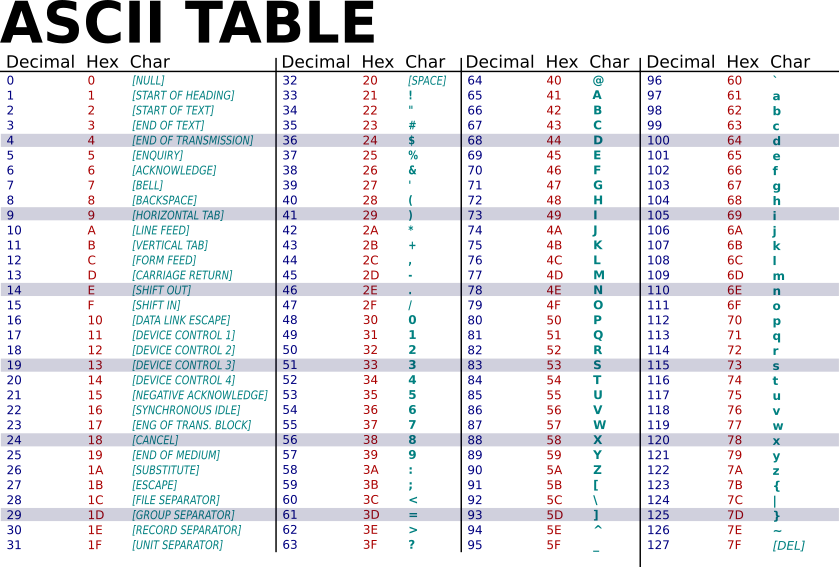
\includegraphics[width=\linewidth]{./gfx/ASCII_table}\newline
\caption
	[ASCII-Codes]
	{ASCII: American Standard Code for Information Interchange\newline
         Source: \url{https://commons.wikimedia.org/wiki/File:ASCII-Table-wide.svg}
    }
\label{fig:ASCII}
\end{figure}

Texts -- \ie strings of letters and other symbols -- are simply sequences of numbers that can be interpreted according to this (or another) table. One nice way of seeing ASCII texts as them being one single number, represented in base 128.

\begin{plusbox}[Other Encodings]
ASCII has been used for a long time, since it can encode most texts with minimal overhead. Especially the \emph{one byte is one character} property means it is easy to work with ASCII text. However, this encoding is rather limiting: there are more than 128\citationneeded. Of course it is possible to come up with a longer table and list more characters in it. Essentially, this is the main idea behind Unicode. However, longer tables mean bigger numbers and therefore break the \emph{one byte is one character} property. This also requires some extra thought in order not to waste memory, make texts recoverable even when communication between two machines is flawed or when different communication standards are used.

If you are inclined to learn more, feel free to look up the keyword UTF-8, which is one \emph{encoding system under Unicode}.
\end{plusbox}

\subsection{Graphics and Sound}
A picture can be understood as a collection of pixels in a given order. So a list of pixel data (together with width and height of the complete image) can be used to encode an image. Each pixel is then defined by its colour, which we could again represent by a single number from a table. As there are a lot of colours\citationneeded, it is more convenient to use analogies to the physical world in which these pictures exist to encode the information.

In the case of pictures, we use the fact that humans have photoreceptors for red, green and blue light. Different intensities in these three categories yield the impression of different colours. Hence, storing three numbers per pixel -- one per \enquote{channel} -- is a great way of putting graphical information in memory.

Similarly, sound can be understood as air pressure varied over time. A microphone effectively measures the air pressure over time and reports the current value back to the processing unit (\eg a stero system or a computer). Recording the air pressure every millisecond (and simply ignoring the values in between) is an apt way to store sound information.

\subsection{Computer Programs} \label{sec:assembly}
Much like characters, the various functions a CPU (\emph{central processing unit}) provides are enumerated. There is a command for \emph{load a value from memory into the processor}, another one for \emph{add two values in the processor} and another one for \emph{write a value from the processor buffer into memory}. The very first programmers really had to know (or constantly look up) the numbers of the various commands; their codes were nothing more than long columns of numbers that got fed directly into the processor.

Obviously, this mode of working is rather tedious. A first improvement was to associate each processor command with a short textual representation (a so called \emph{mnemonic}) that is easier to memorize than numbers. A computer program could then \emph{parse} a text file comprising of these mnemonics and translate them into \emph{machine code}. Such a program is called an \emph{assembler}.

While the concept \emph{enumerated commands} holds for all types of CPUs, there is no universal list which number denotes which command. Even worse, different processors have a different \emph{instruction set}, \ie there are different operations that different hardware can execute. Assembly code written for one processor may not be compatible with a different one. There is no \emph{binary compatibility} between different machines. To circumvent this problem, more abstract (and therefore closer to human thinking) languages have been develloped. Code in these languages is \emph{compiled} into assembly code which then can be translated into machine code. Again, this compile step is performed by a dedicated program, the so called \emph{compiler}. The advantage is, that code has to be written only once and can then be deployed on any hardware, for which a compiler exists.

Compiled languages -- like C -- are also more abstract and therefore closer to the way a human thinks. Rather than programming everything on the electronics level, a programmer can focus more on the \enquote{big picture}. Writing code in assembly language is very demanding, the more so if the program has many features and requires large, interconnected code sections. It is very uncommon to write code directly in assembly\footnote{The first generation of the Pokémon gameboy series was written in assembly. While definitely a noteworthy exploit, the many bugs and glitches these games are known for illustrate the difficulty of the feat.}.

I have already hinted at the possibility to load a value from memory into the processor. Of course, for this, the processor needs to know, \emph{which value} to load. You can imagine the memory of a computer as a long row of enumerated cells. Each cell holds exactly one byte of information. Thus, providing the \emph{address}, \ie the number of a memory cell, suffices to provide just that information. In C, we will be dealing with addresses very frequently.

\section{Generating Executable Files} \label{sec:Compile}
With all this theory behind us, we can finally get to practical matters: generating executable programs!

\subsection{Phases of Translation}
You already know that \emph{translating code into machine language} is a fairly complex process. We have talked about \emph{compiling} (translating from a high level language like C into assembly) and \emph{assembling} (translating from assembly language into machine language). Before compilation, theres also a \emph{preprocessing step}, and at the end of the chain of translation phases, theres \emph{linking}.

\emph{Preprocessing} will be discussed in detail in chapter \ref{chp:Preprocessor}. Essentially it is another translation step that allows to write code in a more convenient way.

\emph{Linking} means combining multiple files of machine language instructions into a single unit of executable code -- think of it as \emph{glueing together the components of a program}.

\subsection{Invoking the Compiler}
Luckily, all these functions can be executed by a single program (which will invoke other programs to do the four discussed tasks in sequence). This program is the \texttt{gcc}. It combines a preprocessor, compiler, assembler and linker in one program. For convenience, it is usually only referred to as \emph{the compiler}; \emph{to compile} most often means the complete chain of four operations that are needed to generate an executable file.

Naively attempting to start it from the command line will result in an error message:
\begin{cmdbox}[Invoking the compiler without argument]
\$ gcc\\
gcc: {\color{red}fatal error}: no input files\\
compilation terminated.
\end{cmdbox}

That is because, if you want something translated into machine language, you need to tell what this something is. So, assuming we have a file called \texttt{mycode.c} in the current working directory in which there is valid C code, you can tell the gcc that you want to compile that very file by simply passing the filename as a command line argument:
\begin{cmdbox}[Invoking the compiler with argument]
\$ gcc mycode.c
\end{cmdbox}

\begin{warnbox}[Avoid whitespaces in filenames]
You see that whitespaces are what separates the command (\texttt{gcc}) from its arguments (in this case, the file name \texttt{mycode.c}). There can be multiple files that go into one project, and there are also other compiler options which we'll discuss in a minute.
\end{warnbox}
%
\begin{warnbox}[]
Since all arguments are supposed to be separated by whitespaces, file names with whitespaces are a problem. You can tell the system that a filename contains whitespaces by wrapping the entire name in double quotes:
\begin{cmdbox}[Compiler invocation on a file name with whitespaces]
\$ gcc \textbf{"}my code.\textbf{c"}
\end{cmdbox}

However, it is easier to avoid whitespaces in filenames alltogether.
\end{warnbox}

Provided that the code in \texttt{mycode.c} is syntactically correct (\ie can be translated at all), an output file with the name \texttt{a.out} (under Linux and MacOS) or \texttt{a.exe} will be generated. There will be no output on the console, \ie no error messages (nor success messages). To execute the final result, simply type...
\begin{tcbraster}[raster columns=2,
                  raster equal height,
                  nobeforeafter,
                  raster column skip=0.2cm]
\begin{cmdbox}[Executing a program in Linux/MacOS]
\$ ./a.out
\end{cmdbox}
%
\begin{cmdbox}[Executing a qprogram in Windows]
\$ a
\end{cmdbox}
\end{tcbraster}

If you want to write the compiled output into a different file, you can prepend the command line option \texttt{-o <outputname>}. So for example, to generate a file with the name \texttt{myexecutable}, type:
\begin{cmdbox}[Setting the output filename]
\$ gcc mycode.c \textbf{-o myexecutable}
\end{cmdbox}

\begin{warnbox}[Extensions matter]
I hope you noticed the \texttt{.c} at the end of the code filename. This \emph{filename extension} is not optional. The extension specifies what kind of content can be found in the file. We will soon see that the compiler can process other types of data than C code; to distinguish between how to process different inputs it needs this file extension.

Likewise, the extension of the generated output file should either be \texttt{.exe} if you work on a Windows machine, or none at all on Linux and Mac.
\end{warnbox}

The chain: preprocessing-compiling-assembling-linking can be stopped after the assembly step. The result is a file that contains machine language, but is not directly executable code. This can be useful if some part of the code is used in multiple projects; one can then translate this shared code only once and only do the last step (linkage) with these \emph{precompiled routines}. To do so, one prefixes the command line flag \texttt{-c} to the code file that should be compiled but not linked:
\begin{cmdbox}[Compiling without linking]
\$ gcc \textbf{-c} mycode.c
\end{cmdbox}

After doing so, you will find the file \texttt{mycode.o} on your hard drive. It is called an \emph{object file} and contains the precompiled routines in machine language. Of course, one can combine this with the \texttt{-o} flag to set the output name. For example, \texttt{gcc -c mycode -o myPrecompiledRoutines.o} is a valid command.

These object files can be passed on to the gcc. Since the extension \texttt{.o} marks them clearly as object files, the gcc knows that they only need to parttake in the linkage step. For example, we could run the following two lines:
\begin{cmdbox}[Generating and using object files]
\$ gcc -c sharedRoutines.c -o routines.o \\
\$ gcc mainProject.c \textbf{routines.o} -o projectExecutable
\end{cmdbox}

Some collections of routines are pre-installed on your computer. These collections are called \emph{libraries} and are really only object files packed together. Usually, their filenames begin with the prefix \texttt{lib} and have the extension \texttt{.a}; the name of the library itself is wedged in between. To use these routines in own programs, we can add them add them to the linkage step with the compiler option \texttt{-l<libname>}, where \texttt{<libname>} is the name of the library we want to use. For example, theres the \emph{math library}, which contains routines that help with common mathematical problems such as computing trigonometric functions or finding the square root. This library has the filename \texttt{libm.a}; the \texttt{<libname>} part hence is really only the letter \texttt{m}. It can be added to a project with:
\begin{cmdbox}[Linking against the math library]
\$ gcc myCode.c \textbf{-lm}
\end{cmdbox}
We will use this library frequently in this course.

In the preface I mentioned in passing that the C programming language is still evolving. Over the last fifty years, some features have been added and also some behaviours were changed in a fundamental way. In order to be able to do both, compile old code as it was intended when it was written and use newer features at the same time, the gcc has a \enquote{switch} that allows to select one of several \emph{standards}. For this, we use the command line parameter \texttt{-std=<standard>}, where \texttt{<standard>} specifies which version of the language should be expected. In this course, we'll be using the Standard from 2017, which goes by the code \texttt{c17}. So, our invocations of the compiler will need the according option set every time:
end um \texttt{-std=c11}:
\begin{cmdbox}[Compiling with the language standard from 2017]
\$ gcc \textbf{-std=c17} myCode.c
\end{cmdbox}

As humans, we are prone to making errors. \emph{Very} prone. I started programming as a hobby more than twenty years ago, and still I hardly write more than some ten lines of code before I check whether I've made any mistake. And there are many mistakes one can make. Some simply render a program \enquote{nonsensical}, \ie prevent translation into machine language alltogether. Others are more subtle; they are valid instructions, but have unintended side effects. The gcc is actually capable of detecting some patterns in code files that were most likely not intended by the programmer. If such patterns are detected, a \emph{warning} is printed on the console -- at least if enabled by the appropriate command line options. Since there are different \enquote{levels of warnings}, there are multiple options: \texttt{-Wall} enables \emph{all} basic warnings; \texttt{-Wextra} adds some more warnings, and \texttt{-Wpedantic} requires the programmer to adhere to a very strict ruleset.

Maybe you're much smarter than I am and don't need this sort of assistance; I for one have been very happy about these features. More often than not they prevented bugs or made me aware of problematic constructs. Therefore, I highly recommend you to compile your codes with these three options:
\begin{cmdbox}[Enabling useful warnings]
\$ gcc \textbf{-Wall -Wextra -Wpedantic} myCode.c
\end{cmdbox}

Since all of this is quite a mouthful to retain, you can look up all of these and other options in the appendix. See table \ref{tab:CompilerOptions} at the end of this book.

To put it in a nutshell, when writing code I recommend you to type these commands; they will soon enough become a second nature:
\begin{cmdbox}[My standard compiler invocation]
\$ gcc -std=c17 -Wall -Wextra -Wpedantic myCode.c -lm -o executable \\
\$ ./executable
\end{cmdbox}

\section{Main Takeaways} 
\begin{itembox}[Binary Data]
\item All information is stored as bitpatterns that have no inherent meaning. What a given sequence of bits means depends on which interpretation rules are applied
\item All information is grouped in bytes, \ie groups of eight bits. Multiple bytes can be compounded to form a larger piece of information.
\item There is a principal difference between integers and floating point numbers.
\end{itembox}
%
\begin{itembox}[Translating Code]
\item C code is translated into executable files in four steps: preprocessing, compiling, assembly and linkage. The gcc can do all these steps in one go.
\item C code files need to have the extension \texttt{.c}.
\item C code can be compiled once into object files and used in several projects. Object files have the extension \texttt{.o}
\item Libraries are collections of object files that can parttake in the linkage process. To do so, use the option \texttt{-l<library name>}
\item Depending on the operating system, executable files should either have no extension (Linux, Mac) or the extension \texttt{.exe}
\item To set an output name, use the option \texttt{-o <output filename>}
\item There are different language standards for the C programming language. A standard can be selected with the option \texttt{-std=<standard>}. We use \texttt{-std=c17} in this course.
\item The compiler can analyze the code for suspicious lines that most likely generate undesired behaviour. To enable this feature, add the compiler options \texttt{-Wall -Wextra -Wpedantic}.
\end{itembox}

\section{Exercises and Solutions}
\subsubsection*{Translating Binary}
\begin{itemize}
\item Which positive integer corresponds to the bit sequence $101010_2$?
\item Which bit sequence corresponds to the decimal number $21_{10}$?
\item Which bit sequence corresponds to the string \texttt{42}?
\end{itemize}

\subsubsection*{Pitfalls in binary encoding}
\begin{itemize}
\item Why does it matter for a computer whether a number is given as $2.0$ or as $2$?
\item You are given a sequence of 16 bits together with the information that they encode an unsigned integer. Why is even this information not enough to unambiguosly decode the bit sequence?
\end{itemize}

\rule{\linewidth}{0.1mm}

\subsubsection*{Solution: Translating Binary}
\begin{itemize}
\item $101010_2 = 42_{10}$
\item $21_{10} = 10101_2$. \\
	Notice how $42 = 2 \times 21$ and how, in binary, you get from $21$ to $42$ by adding a zero.\\
	Do you see how this is related to the fact that $2_{10} = 10_2$?\\
	(Multiplying with ten in the decimal system also only adds a zero to the number representation)
\item The \emph{string} \texttt{42} comprises of two \emph{characters}, \texttt{4} and \texttt{2}.\\
	From the ASCII table (fig. \ref{fig:ASCII}) we find that \texttt{4} has codepoint 52 and \texttt{2} has codepoint 50.\\
	Converting these codepoints into binary gives the bit sequence \texttt{0011 0100  0011 0010}.
\end{itemize}

\subsubsection*{Pitfalls in binary encoding}
	\chapter{Writing C Code}
\epigraph{The secret to getting ahead is getting started.}{Mark Twain}

In this chapter, we'll discuss the principal structure of a C language program by analyzing a so called \emph{Hello World} -- a program which has the sole purpose of putting the text \emph{Hello World} on screen\footnote{The expressin \emph{Hello World} is also used in context of other languages. This \enquote{most simple} possible program is commonly used as a sort of reference, a way to compare programming languages -- or to simply fool around. People have made s sport out of writing programs that essentially are Hello World variations but don't look like anything made for human eyes at all. See, for example, \url{https://codegolf.stackexchange.com/questions/22533/weirdest-obfuscated-hello-world}}.

Once we've familiarized ourselves with this primary structure, we'll start writing actually useful code by making simple calculations in C.

\section{A First Program: Hello World}

The following lines show code that prints the text \texttt{Hello World} on screen:
\begin{codebox}[helloworld.c]
\begin{minted}[linenos]{c}
#include <stdio.h>

int main() {
   printf("Hello World!\n");
}
\end{minted}
\captionof{code}{A Hello World} \label{code:helloworld}
\end{codebox}

To compile and run it, remember the compiler invocation:

\begin{cmdbox}[Compiling and Executing the Hello World]
\$ gcc -std=c17 -Wall -Wextra -Wpedantic helloWorld.c -o helloWorld \\
\$ ./helloWorld \\
Hello World!
\end{cmdbox}

Now let's go through code \ref{code:helloworld} line by line.

We've already discussed that recurrent tasks can be externalized and put into a library. Input and Output fram and to the console is such a recurrent task. The routines concerned with these tasks are implemented in the \emph{C standard library}, which is automatically included in the linkage process -- no need to use a compiler option. However, these pre-compiled routines are, well, compiled, \ie translated into machine language. In this process, some information is lost that would allow for direct integration in our code. To provide this lost information, a so called \emph{Header File} needs to be \emph{included} into our code. For the time being, don't concern yourself with what this means in detail too much; simply think of a header file as a sort of glue that helps combining your C-Code to machine language code somewhere else.

After these explanations, you can probably guess that in line 1 we include this header file. The command \texttt{\#include} loads a file from the hard disk, and copy-pastes it into the C-code file. The file to load is specified in <angle brackets>\footnote{In chapter \ref{chp:Preprocessor}, we'll see that there are other options, too -- but let's not get ahead of ourselves.} This also constitutes a preprocessor operation: line 1 is replaced by the content of the file \texttt{stdio.h} by the preprocessor. All \emph{preprocessor directives} begin with a pound symbol (\texttt{\#}).

Programs are organized into subroutines or \emph{functions}, \ie smaller sections of code that form the building blocks of the whole. Line 3 \emph{declares} such a function. It has the name \texttt{main}. The \emph{body} of the function (\ie its \enquote{content}) is enclosed by \{curly braces\}. All code but a very few needs to be placed within functions, so we'll see this pattern in every program we'll see throughout our C coding days. Functions can have virtually any name, but the name \texttt{main} is special: it marks the, well, \emph{main} function, \ie the starting point for our program. When there are multiple functions, all of them but the \texttt{main} function are \enquote{ignored} until you as a programmer explicitly \emph{call} them -- but we'll hear more about that in chapter \ref{chp:funcs}. For now, accept simply that the line \inC{int main ()} marks the starting point for the \enquote{proper} code, which you will find within \{braces\}.

The only line left to understand is line 4. It contains a \emph{statement}, \ie a command that can be executed, and this statement is a \emph{call to the function \texttt{printf}}. That means, somewhere (in the precompiled standard library), there is another function with the name \texttt{printf}. The code there can be used to make output on screen (the \texttt{f} in the function's name stands for \emph{formatted} -- we'll see later, why that is). Of course, the routine needs to know \emph{what text} should be put on screen. To distinguish the \emph{function arguments} (\ie the information sent or \emph{passed} to the function) from the rest of the code, they are enclosed by (parens). In general, we can pass all kinds of information into functions. In the previous chapter, we've already heard that there is some ambiguity as to how to interpret \enquote{raw information}. In particular, we've seen that text is treated differently from numbers. But also when we're dealing with text (like our C code), there can still be different ways to interpret them. \texttt{Hello Word!} could be the text we want to print on screen, or some C code that needs to be translated into machine language. Since the computer can't guess our intent (remember our mantra from the preface?), we need to be explicit: we mark the text we want to put on screen as \emph{literal text} by enclosing it in a pair of \texttt{"}quotation marks\texttt{"}.

While this makes it clear what is code and what is literal text, it also introduces some minor problems. Say, you want to have some text that also includes quotation marks. There needs to be a way to tell the compiler that a double quote in the code is not to be interpreted as end of text delimiter but as part of the text. This is done by \emph{escape sequences}: special substrings in a text that are not taken verbatim but interpreted in a different (simple) way. In C, escape sequences begin with a backslash (\textbackslash) followed by usually one chacracter. For example, the sequence \texttt{\textbackslash"} becomes such a quotation mark within the text.

In line four, we find the escape sequence \texttt{\textbackslash n}; this encodes a line break (\texttt{n} stands for \emph{new line}). Unfortunately, literal texts cannot span multiple lines, so for the time being, these escape sequences are the only way to make multiline output. See table \ref{tab:Escape} in the appendix for more escape sequences.

Note also that line four ends with a semicolon (;). This ends the statement. Each statement needs to end in a semicolon, otherwise, you'll find that gcc refuses to compile your code and outputs an error message.

\begin{cmdbox}[Error message when compiling \texttt{helloworld.c} without semicolon in line 4]
\begin{minted}{text}
helloworld.c: In function ‘main’:
helloworld.c:4:29: error: expected ‘;’ before ‘}’ token
    4 |     printf("Hello World!\n")
      |                             ^
      |                             ;
    5 | }
      | ~
\end{minted}
\end{cmdbox}

This is because (unlike literal strings) statements can be spread over multiple lines. Similarly, there can be more than one statement in a single line. As programmers, this gives us some liberty in formatting the code such that it can be read more easily. Also, we can add or remove whitespaces (or tabs) pretty much anywhere, as long as we keep \enquote{words} together. The following code produces the same output as code \ref{code:helloworld}
\begin{codebox}[Code with optional whitespaces added]
\begin{minted}[linenos]{c}
  #include     <stdio.h>
 int    main   (   )    {
      printf   (   
         "Hello World!\n"
)   ;
   }
\end{minted}
\captionof{code}{A Hello World with added whitespaces} \label{code:optionalWhitespaces}
\end{codebox}

\begin{hintbox}[Rule of thumb: whitespaces]
The added whitespaces in code \ref{code:optionalWhitespaces} are meant to illustrate where it is allowed to add them; clearly, this example makes the code look more like a random image than an organized list of instructions. This is not to say that \emph{indenting} your code is a bad idea. Quite to the contrary, these whitespaces and extra line breaks can help you a lot in visualizing relationships between different parts of the code or filter relevant information. This becomes paramount once our codes reach some complexity.

As a rule of thumb, you should add a level of indentation for every opening brace (\{\}), paren () or bracket ([ ]) that is not closed in the same line. Furthermore, the second to last line of statements that take more than one line of code should also be indented.

It is up to you, how many whitespaces (or tabs) you add; only you should stay consistent throughout your code. Commonly, one indentation level means four white spaces, but also two or eight whitespaces are not unheard of. Many code editors can be configured to automatically indent to the next multiple of two, four or eight whitespaces on the press of the tabulator key.

In this book I'll do my best to stay consistent in my indentation style. You may take this as inspiration for your own code.
\end{hintbox}

The gcc reads the code \enquote{from top to bottom}. This means that the order of statements is of great importance. If, for example, you move the \inC{#include} statement from line 1 to the end of the code, you'd get an error message. The reason behind this is that the command \texttt{printf} is only declared in the fine \texttt{stdio.h}; before this declaration, the compiler \enquote{doesn't know} what \texttt{printf} even means.

\section{Variables, Data Types, Operators} \label{sec:expressions}
\emph{Useful} programs evolve over time. They compute some result or react to user input. To realize such dynamicity, C allows the existens of \emph{variables}, \ie stored information that can change over time. In this section we'll learn how to create and use variables and some of the \enquote{behind the scenes}, \ie what happens in memory when we use them.

\subsection{Memory Structure}
Imagine the memory as a long chain of enumerated cells. Each cell holds one byte's worth of information, \ie eight bits. These cells can never be empty; there's always \emph{some} information stored in them, albeit possibly nonsensical or useless. If we want to make use of this structure, someone or something will have to keep track of which cells hold which pieces of information, and how to interpret them.

Luckily, most of this bookkeeping is done automatically by the compiler; to properly utilize its features, however, we need to clarify some names.

Within the cells, we find \emph{values}. As mentioned, they are, a priori, pure bitpatterns with no inherent meaning. Provided we know \emph{what sort of information} they encode, we can make sense of these bitpatterns.

The question \emph{what sort of information} is contained in a cell is called \emph{data type}. The data type is a name for both, the method of interpretation of the raw data in the cells, as well as the \emph{number of bytes per unit of information}. From the previous chapter, you remember how to interpret bit patterns as signed integers; to do so, you also need to know how many bytes to consider in your interpretation. A \emph{32bit signed integer} is thus a data type.

The value we are looking for is in one of the enumerated cells. The \enquote{number of the cell} in which a given value is stored is its \emph{address}. An address itself can be stored as some unsigned integer. Adresses often are expressed as \emph{hexadecimal numbers}. That means, the number is written in base 16. You'll not only find the digits 0..9, but also A, B, ..., F (or, sometimes, the lower case letters a .. f). The digit 'A' then has the decimal value 10, 'B' is 11 and so on. The transformation back into base ten works just like described in section \ref{sec:BinaryNumbers}. To make sure a number is given in hexadecimal, it often carries the prefix \texttt{0x}. More often than not, the exact value of addresses is of little importance; if you ever see hexadecimal numbers, simply know that they are just another way of writing normal decimal numbers.

As humans, we prefer symbols over addresses. \emph{The value of cell 238} doesn't tell a lot about its content or what it means. In contrast, \emph{the value of \texttt{nameOfPlayer1}} clearly signifies some textual information. We call \texttt{nameOfPlayer1} a \emph{symbol}. It is a stand-in for the address of the cell(s), in which the name of player 1 can be found. The compiler \emph{binds} the symbols we as humans choose to the addresses in memory.

\begin{defbox}[Memory Image]
\begin{center}
\begin{tikzpicture}
  [
    cell/.style={text width=8mm,
      text height=4mm, draw=black, inner sep=1mm},
    ld/.style={draw=blue,shorten >=2pt,->}
  ]
  \node (c1) at (0,0) [cell] {\ttfamily 99};
  \node (c2) at (1,0) [cell] {\ttfamily 1};
  \node (c3) at (2,0) [cell] {\ttfamily 255};
  \node (c4) at (3,0) [cell] {\ttfamily 0};
  \node (c5) at (4,0) [cell] {\ttfamily 80};
  \node (c6) at (5,0) [cell] {\ttfamily ...};

  \node (labelMem) at (8,  1) {Symbols in our Code};
  \node (labelMem) at (8,  0) {Values in memory};
  \node (labelMem) at (8, -1) {Addresses};

  \node (a1) [below=2mm of c1]            {\tiny 0x27ff};
  \node (a2) [below=2mm of c2, color=red] {\tiny 0x2800};
  \node (a3) [below=2mm of c3]            {\tiny 0x2801};
  \node (a4) [below=2mm of c4]            {\tiny 0x2802};
  \node (a5) [below=2mm of c5]            {\tiny 0x2803};
  \node (a6) [below=2mm of c6]            {\tiny 0x2804};

  \node (ptr) [below=8mm of c1] {\scriptsize Address of \texttt{x}};
  \node (vc2) [above=6mm of c1] {\scriptsize Variable \texttt{x}};
  \node (vc0) [above=2mm of c1] {\scriptsize Variable \texttt{y}};

  \draw [ld] (ptr.east) .. controls +(0.3,0) .. (a2.south);
  \draw [ld] (vc0.east) .. controls +(0.4,0) .. (c2.north);
  \draw [ld] (vc2.east) .. controls +(2.4,0) .. (c4.north);
\end{tikzpicture}
\end{center}
\captionof{figure}{Variables in memory}
\end{defbox}

\subsection{Declaring Variables} \label{sec:DeclareVars}
To use variables in our code, we first have to \emph{declare} them. That means we have to tell the compiler that we want a variable and what kind of variable this should be. We do that with a statement of the form:
\begin{codebox}[Syntax: Declaring variables]
\texttt{dataType symbolName;}
\end{codebox}

\texttt{dataType} stands for one of several registered keywords of the C programming language. Section \ref{sec:Datatypes} in the appendix lists all predefined data types. For the most part, we can limit ourselves to using one of these three:
\newpage
\begin{center}
\newcolumntype{T}{>{\centering\ttfamily\arraybackslash}m{.2\linewidth}}
\newcolumntype{U}{>{\centering \arraybackslash}        p{.3\linewidth}}

\rowcolors{1}{white}{tabhighlight}
\begin{tabularx}
	{.5505\linewidth}
	{TU}
\toprule[1.5pt]
	\textbf{\textrm{data type}} & \textbf{use} \tabcrlf
	int                         & integers \\
	double                      & floating point numbers \\
	char                        & characters \\
\bottomrule[1.5pt]
\end{tabularx}
\captionof{table}{The most commonly used data types in C}
\end{center}

\texttt{symbolName} is an arbitrary identifyer we can choose, like \texttt{nameOfPlayer1}. It must abide to these rules:
\begin{itemize}
\item Must only comprise of the characters \texttt{a..z}, \texttt{A..Z}, \texttt{0..9} or \texttt{\_}
\item The first character must not be a digit
\item Must have at most 40 characters
\item Must be unique (there may not be two symbols with the same name in the same section. For example, it is not allowed to have a variable named \texttt{main} 
	since there has to be a function with that name\footnote{\emph{Technically}, there is a way around that... practically... \url{https://xkcd.com/1475/}}.)
\end{itemize}
The language C is \emph{case sensitive}, \ie there is a difference between \texttt{nameOfPlayer1} and \texttt{NameOfPlayer1}. By convention, variable names start with a lower case letter. If a variable comprises of several human language words (like \texttt{nameOfPlayer1}) one often applies \enquote{camel case}, \ie begin each new word in the symbol with an upper case letter (except for the first one). An alternative is \enquote{snake case}, where the individual words are separated by underscores (\texttt{name\_of\_player\_1}). Which of the two conventions you pick is up to you; again I only advise you to be consistent in your choice (otherwise you'll have a hard time remembering whether you spelled it \texttt{paragraph\_index} or \texttt{paragraphIndex}.)

\begin{hintbox}[Good names]
A common \enquote{mistake} among beginners is to use inexpressive names such as \texttt{x}, \texttt{y}, \texttt{a}, ... While this is no problem for the compiler (note the quotation marks around \enquote{mistake}), it makes codes harder to write, maintain and debug. Programming becomes quite complex very soon, and the last thing we want is loosing track of whether \texttt{a} is the total score or which meaning behind the variable \texttt{b}.

Instead, be as descriptive as possible when giving names. A guideline to follow is \emph{good code should read like prose text}. That certainly is only possible if the variables are named after human concepts like \texttt{repetitions}, \texttt{message}, \texttt{velocity\_x}, ...
\end{hintbox}

A \emph{declaration} (\ie a line like \inC{int number;}) does two things: it \emph{reserves memory} (\ie it picks a number of consecutive cells in memory and tells the operating system that they are used now) and \emph{binds it to the symbol} (\ie the compiler knows that \texttt{symbolName} should refer to the content of the reserved memory cells).

Multiple variables \emph{of the same type} can be declared in a single statement\footnote{However, this programming style is sometimes discouraged.}. To do so, we list them separated by commas. A valid declaration of variables could thus look like this:
\begin{codebox}[Declaration of variables]
\begin{minted}[linenos]{c}
int main () {
   int    count;
   double positionX, positionY;
}
\end{minted}
\captionof{code}{Declaration of variables}
\end{codebox}

You may have noticed the similarity between the definition of the variable \texttt{count} and the function \texttt{main}. That is no coincidence! From the viewpoint of the compiler, the function \texttt{main} is a set of instructions to compute an \inC{int}. We'll learn more about this in chapters \ref{chp:funcs} and \ref{chp:OS-Link}.

\begin{warnbox}[Avoid global variables]
Note that the declaration of the variables \texttt{count}, \texttt{positionX} and \texttt{positionY} is \emph{within} the function \texttt{main}. We \emph{could} also define them outside of \texttt{main}; but this would potentially lead to a lot of trouble. We'll discuss the implications of that placement in chapter \ref{chp:funcs}. For now, just stick to the rule:

Anything that is not an \texttt{\#include} line must be \emph{within} the braces that belong to \inC{int main}.
\end{warnbox}

%TODO
% essentially keep structure of chapter 2, ...
% but introduce mem structure and pointers here already (take from chapter 3)
% move xkcd: 1000 in here, after def: hex. ... or leave it in C3
% C3 becomes: casting, pointer access, bit magic


\subsection{Wertezuweisung} \label{sec:valueAssignment}
Werte können über den \emph{Operator} = zugewiesen werden:
\begin{codebox}[Beispiel: Wertzuweisung]
\begin{minted}[linenos]{c}
int main () {
    int    Ganzzahl;
    double Kommazahl, andereZahl;

    Ganzzahl   = 7;
    Ganzzahl   = 8;

    Kommazahl  = 4.3;
    andereZahl = 5.0;
}
\end{minted}
\end{codebox}

In Zeile 5 wird also der Variablen \texttt{Ganzzahl} der Wert 7 zugewiesen. In der folgenden Zeile 6 überschreiben wir diesen Wert mit dem Wert 8.

In den Zeilen 7 und 8 erhalten die beiden \mintinline{c}{double}-Variablen ebenfalls Werte. Wir bemerken, dass hier ein \emph{Dezimalpunkt} gesetzt wird, also kein Komma.

Deklaration und Wertzuweisung können auch in einem einzigen Schritt geschehen:
\begin{codebox}[Beispiel: Kombinierte Deklaration und Wertzuweisung]
\begin{minted}[linenos]{c}
int main () {
   int    Ganzzahl   = 8;
   double Kommazahl  = 4.3,
          andereZahl = 5.0;
}
\end{minted}
\end{codebox}

\begin{hintbox}[Nicht-Initialisierte Variablen]
Wenn eine Variable deklariert wird, sorgt der Compiler lediglich dafür, dass genug Platz im Speicher reserviert wird, um diesen Wert zu erfassen. Im Allgemeinen wird aber kein bestimmter \enquote{Startwert} festgelegt. Die neue Variable startet mit dem Wert, den das Bitmuster an der Stelle festlegt, an der Platz für die Variable reserviert wurde. Dies ist ein zufälliger Wert! Programme, die mit einem solchen Zufallswert weiterarbeiten haben generell \emph{undefiniertes} Verhalten und können abstürzen oder sogar Schaden anrichten. Es ist daher also ratsam, allen Variablen bei der Deklaration gleich einen sinnvollen oder sicheren Startwert zuzuweisen.
\end{hintbox}

\begin{hintbox}[Fließkommazahlen ohne Nachkommastelle]
In der Mathematik gilt $5 = 5.0$. Ein Computer arbeitet zwar nach mathematischen Prinzipien; streng genommen gilt diese Gleichheit für den Prozessor aber nicht. Wie wir in Abschnitt \ref{sec:DataRepresentation} sehen werden kann dieselbe (mathematische) Zahl auf verschiedene Weisen binär dargestellt werden. Insbesondere zwischen Ganzzahlen und Kommazahlen bestehen große Unterschiede in der Binär-Darstellung. Der gcc kann zwar Umwandlungen automatisch durchführen, und würde auch
\begin{codebox}[Beispiel: Implizite Typumwandlung von Ganzzahl zu Fließkommazahl]
\begin{minted}[linenos]{c}
int main () {
   double Kommazahl = 5;
}
\end{minted}
\end{codebox}
\enquote{korrekt} umsetzen. Hier wird versucht, die \emph{Ganzzahl} \texttt{5} in der \mintinline{c}{double}-Variablen \texttt{Kommazahl} zu speichern. Da dies direkt nicht möglich ist, wandelt der gcc diese Ganzzahl zuerst in die Fließkommazahl \texttt{5.0} um und speichert dann diese. Eine solche \emph{implizite Typumwandlung} kann aber unbeabsichtigte Nebeneffekte haben und sollte daher vermieden werden. Als Beispiel für solche Nebeneffekte möchte ich Ihnen das folgende Beispiel geben:
\end{hintbox}
%
\begin{hintbox}[]
\begin{codebox}[Beispiel: Implizite Typumwandlung von Fließkommazahl zu Ganzzahl]
\begin{minted}[linenos]{c}
int main () {
   int Ganzzahl = 5.5;
}
\end{minted}
\end{codebox}
Analog zum Beispiel oben wird nun implizit die Zahl \texttt{5.5} zu einer Ganzzahl konvertiert. Natürlich ist Ihnen bewusst, dass es keine ganze Zahl gibt, die gleich $5.5$ ist. Es wird also gerundet. Im Gegensatz zur menschlichen Intuition rundet der gcc hier aber \emph{ab}. Außerdem können die \enquote{fehlenden} $0.5$ das Verhalten des Programms in der Laufzeit gegenüber der Erwartung verändern.

Damit der Datentyp (und damit das Verhalten des Programms) immer ersichtlich ist, sollten daher \enquote{ganzzahlige Fließkommawerte} als Kommawert (\eg \texttt{5.0}) gesetzt werden.
\end{hintbox}

\subsection{Rechnen mit Variablen -- Operatoren}\label{sec:OperatorsArithmetic}
Mit Variablen kann auch gerechnet werden. Hierzu stehen 6 \enquote{Grundrechenarten} zur Verfügung (siehe Tabelle \ref{tab:OperatorsArithmetic}). Mehrere solche Rechenoperationen können hintereinander geschaltet werden. Es gilt wie üblich Punkt-vor-Strich; Klammern können gesetzt werden um eine andere Reihenfolge festzulegen.
\begin{table}[h!]
	\newcolumntype{C}{>{\ttfamily\centering\arraybackslash} p{.2\linewidth}}
\begin{center}
\begin{tabularx}
	{.95\linewidth}
	{cC|cC}
\toprule[1pt]

	Operation   & \normalfont Zeichen  &  Operation                              & \normalfont Zeichen
\tabcrlf
	Addition    & +                    &  Multiplikation                         & * \\
	Subtraktion & -                    &  Division                               & / \\
	Negation    & -                    &  Rest der Division (\enquote{Modulo})   & \%\\

\bottomrule[1pt]
\end{tabularx}
\end{center}
\caption{Rechenoperatoren in C}\label{tab:OperatorsArithmetic}
\end{table}

\begin{codebox}[Beispiel: Rechnen mit Variablen]
\begin{minted}[linenos]{c}
int main () {
   int    Ganzzahl;
   double Kommazahl, andereZahl;

   Ganzzahl   = 7;
   Ganzzahl   = Ganzzahl + 8;

   Kommazahl  = 4.3;
   andereZahl = 3.0 * (-Kommazahl + 7.9) / 2.0;
}
\end{minted}
\end{codebox}

Wichtig ist, dass Variablen bereits deklariert sind \emph{bevor} auf sie verwiesen wird, \ie bevor sie in anderen Ausdrücken vorkommen. Folgendes Beispiel funktioniert daher nicht:
\begin{codebox}[Beispiel: Fehlerhafter Code{,} Variablen zu spät deklariert]
\begin{minted}[linenos]{c}
int main () {
  Ganzzahl = 7;
  int Ganzzahl;
}
\end{minted}
\end{codebox}
und erzeugt die folgende Fehlermeldung:
\begin{cmdbox}[Fehlermeldungen des gcc]
\begin{minted}{text}
myProgram.c: In function ‘main’:
myProgram.c:2:4: error: ‘Ganzzahl’ undeclared (first use in this
function)
    Ganzzahl = 7;
    ^~~~~~~~
myProgram.c:2:4: note: each undeclared identifier is reported only once
for each function it appears in
\end{minted}
\end{cmdbox}
Jede Fehlermeldung beginnt mit einem Verweis auf die fehlerhafte Datei und die Funktion darin, in der das Problem aufgetreten ist (\texttt{myProgram.c: In function ‘main’:}). In der folgenden Zeile der Fehlerausgabe wird genauer spezifiziert in welcher Zeile, und an welcher Stelle der Fehler auftrat (\texttt{myProgram.c:2:4}, also  Zeile 2, Spalte 4) und welcher Fehler gefunden wurde (\texttt{‘Ganzzahl’ undeclared}). Schließlich gibt der Compiler noch die relevante Stelle aus und markiert diese erfreulicherweise.

\begin{hintbox}[Zur Division mit Ganzzahl- und Fließkomma-Werten]
Der Datentyp einer Division hängt vom Datentyp von Divisor und Dividend ab. Ist einer der beiden ein Fließkommawert, so wird auch das Ergebnis als Fließkommawert berechnet. Sind beide Werte Ganzzahlen, wird auch das Ergebnis als Ganzzahl berechnet und gegebenenfalls abgerundet. Betrachten wir folgendes Beispiel:
\begin{codebox}[Beispiel: Division von Ganzzahlen und Fließkommazahlen]
\begin{minted}[linenos]{c}
double x = 3   / 2  ,
       y = 3.0 / 2.0,
       z = 3.0 / 2  ,
       w = 3   / 2.0;
\end{minted}
\end{codebox}
Die Variable \texttt{x} geht aus der Division zweier Ganzzahlen hervor, und wird damit zu \texttt{1.0} abgerundet. Bei der Berechnung von \texttt{y} hingegen gehen Fließkommazahlen in die Division ein; somit wird das Ergebnis nicht gerundet und als 1.5 gespeichert. Dasselbe gilt für \texttt{z} und \texttt{w}, da zumindest \emph{eine} der an der Division beteiligten Zahlen eine Fließkommazahl war.
\end{hintbox}

\subsection{Shorthands}
%TODO prefix and postfix form
Häufig soll sich der Wert einer Variablen \emph{inkrementiert} (\enquote{hochgezählt}) werden. Dies kann codiert werden als:
\begin{codebox}[Beispiel: Inkrementieren einer Variablen i]
\begin{minted}[linenos]{c}
int main () {
   int i = 5;
   i = i + 1;  // i hat jetzt den Wert 6
}
\end{minted}
\end{codebox}

Daneben gibt es auch den \emph{Shorthand} (Kurzform) \texttt{variable++}:
\begin{codebox}[Beispiel: Inkrementieren einer Variablen i mit Shorthand ++]
\begin{minted}[linenos]{c}
int main () {
   int i = 5;
   i++;       // i hat jetzt den Wert 6
}
\end{minted}
\end{codebox}

In beiden Beispielen wird der Wert von \texttt{i} in Zeile 3 um 1 erhöht.

Analog dazu existiert der \emph{Dekrement}-Operator \texttt{variable-{}-}, der den Wert von \texttt{variable} um 1 verringert.

Weiter existieren der Operator-Shorthand \texttt{variable += expression}. Zu \texttt{variable} wird der Wert von \texttt{expression} hinzugezählt und anschließend in \texttt{variable} gespeichert. \texttt{expression} darf dabei ein beliebig komplexer Ausdruck sein:
\begin{codebox}[Beispiel: Inkrementieren einer Variablen i mit Shorthand \texttt{+=}]
\begin{minted}[linenos]{c}
int main () {
   int i = 5,
       j = 2;
   i += 3 * j + 1;     // i = i + 3 * j + 1
}
\end{minted}
\end{codebox}
Hier wird zunächst der Ausdruck \texttt{3 * j + 1} ausgewertet zu \texttt{7}; als nächster Schritt wird die Summe \texttt{i + 7} berechnet, und diese dann in \texttt{i} gespeichert. Die Variable \texttt{i} hat also nach Zeile 4 den Wert 12.

Analog existieren auch die Shorthands \texttt{-=}, \texttt{*=}, \texttt{/=} und \texttt{\%=}.

\begin{hintbox}[Inkrement und Dekrement: Prefix und Postfix]
Die Operatoren \texttt{++} und \texttt{-{}-} können sowohl \emph{vor} als auch \texttt{hinter} einen Ausdruck gesetzt werden (wir sprechen von \emph{Prefix} und \emph{Postfix}). Für sich alleine ist in beiden Fällen der Effekt derselbe -- der Wert des Ausdrucks wird um 1 erhöht bzw. verringert. Kombiniert mit anderen Operationen ergeben sich aber Unterschiede. Betrachten wir folgendes Beispiel:

\begin{codebox}[Beispiel: Unterschiede bei Prefix- und Postfix-Inkrement]
\begin{minted}[linenos]{c}
int main () {
   int i, j;

   // Postfix-Form
   i = 5;
   j = i++;		// i = 6, j = 5.

   // Prefix-Form
   i = 5;
   j = ++i;		// i = 6, j = 6.
}
\end{minted}
\end{codebox}

In der Postfix-Form (Zeile 6) wird zuerst der Wert von \texttt{i} gelesen und der Variablen \texttt{j} zugewiesen; danach wird \texttt{i} inkrementiert.

Bei der Prefix-Form (Zeile 10) dagegen wird zuerst \texttt{i} inkrementiert und danach der Wert von \texttt{i} in \texttt{j} gespeichert.
\end{hintbox}
%
\begin{hintbox}[]
Um den Code leicht les- und wartbar zu halten, empfehle ich, alle gedanklichen Schritte in abgeschlossene Befehle zu setzen. Äquivalent zum obigen Code ist der folgende, intuitiv leichter verständliche Code:

\begin{codebox}[Beispiel: Äquivalente Codes]
\begin{minted}[linenos]{c}
int main () {
   int i, j;

   // zur Postfix-Form
   i = 5;
   j = i;
   i++;		// i = 6, j = 5.

   // zur Prefix-Form
   i = 5;
   i++;
   j = i;		// i = 6, j = 6.
}
\end{minted}
\end{codebox}
\end{hintbox}

\section{Formatierte Ausgabe}\label{sec:formattedOutput}
Wir wollen nun auch die berechneten Ergebnisse in Erfahrung bringen. Dazu können wir den bereits bekannten Befehl \texttt{printf} benutzen. Betrachten wir folgendes Beispiel:

\begin{codebox}[Beispiel: Ausgabe einer Berechnung mit \texttt{printf}]
\begin{minted}[linenos]{c}
#include <stdio.h>

int main () {
   double result = 5.0 / 7.0;

   printf("5.0 / 7.0 = %lf\n", result);
}
\end{minted}
\end{codebox}

Die Ausgabe lautet:
\begin{cmdbox}[Ausgabe einer Berechnung mit \texttt{printf}]
5.0 / 7.0 = 0.714286
\end{cmdbox}

Wie oben besprochen wird zuerst in Zeile 4 das Ergebnis der Division zweier Fließkommazahlen berechnet und in der Variablen \texttt{result} gespeichert. Zur Ausgabe auf dem Bildschirm übergeben wir dem Befehl \texttt{printf} jetzt \emph{zwei} Argumente:

Das erste Argument wird \emph{Format-String} genannt und ist in unserem Beispiel der Anteil:
\begin{center}
\mintinline{c}{"5.0 / 7.0 = %lf\n"}.
\end{center}

Ein Format-String ist eine Zeichenkette die \emph{Platzhalter} enthalten kann. Diese beginnen mit dem Zeichen \texttt{\%} gefolgt von einem oder mehreren Zeichen, die beschreiben, wofür Platz freigehalten werden soll. In diesem Fall steht der Platzhalter \texttt{\%lf}, was für eine \mintinline{c}{double}-Zahl steht. Diese Zahl wird hinter dem Format-String genannt und von diesem durch ein Komma abgetrennt. Weitere Platzhalter-Symbole sind in Tabelle \ref{tab:FormatOutNum} aufgelistet.

In einem Format-String können beliebig viele Platzhalter stehen; für jeden Platzhalter muss eine entsprechende Einsetzung hinter dem Formatstring selbst genannt werden.
\begin{codebox}[Beispiel: Ausgabe mehrerer Werte mit \texttt{printf}]
\begin{minted}[linenos]{c}
#include <stdio.h>

int main () {
   double f = 3.14;
   int    g = 42;

   printf(
      "Ganzzahl i = %d, Fliesskommazahl d = %lf, weitere Zahl = %d",
                    g,                      f,                  99);
}
\end{minted}
\end{codebox}

Werden hinter dem Formatstring zu viele oder zu wenige Werte angegeben, so meldet der Compiler eine Warnung:
\begin{cmdbox}[Warnung bei zu wenigen Argumenten für den Formatstring]
\begin{minted}{text}
myProgram.c: In function ‘main’:
myProgram.c:4:12: warning: format ‘%i’ expects a matching ‘int’ argument
[-Wformat=]
   printf("%i\n");
           ~^
\end{minted}
\end{cmdbox}
Das Programm wird jedoch \enquote{erfolgreich} kompiliert und ausgeführt. Anstelle des Platzhalters wird ein zufälliger Wert vom Speicher eingesetzt\footnote{Bugs dieser Art sind leider häufig. Der im Jahr 2014 entdeckte \emph{Heartbleed-Bug} in der OpenSSL-Library geht auf einen ähnlichen Mechanismus zurück. Hacker konnten \enquote{fehlerhafte Anfragen} an einen Server schicken und so den Speicherinhalt des Servers auslesen -- und damit \eg Zugangsdaten der User auslesen. Compiler-Warnungen sollten also sehr ernst genommen werden.}.

Ähnliches stellen wir fest, wenn wir das folgende Beispiel betrachten:

\begin{codebox}[Beispiel: Ausgabe mehrerer Werte mit \texttt{printf}]
\begin{minted}[linenos]{c}
#include <stdio.h>

int main () {
   printf("%d\n", 1.5);
}
\end{minted}
\end{codebox}
Der Formatstring \texttt{\%d} beschreibt die Ausgabe einer \emph{Ganzzahl}; als Wert für diesen Platzhalter wird aber eine Fließkommazahl angeboten. Die Compiler-Warnung:

\begin{cmdbox}[Warnung bei falscher Zuordnung Platzhalter/Datensatz]
\begin{minted}{text}
myProgram.c: In function ‘main’:
myProgram.c:4:12: warning: format ‘%d’ expects argument of type ‘int’, but
argument 2 has type ‘double’ [-Wformat=]
   printf("%d\n", 1.5);
           ~^
           %f
\end{minted}
\end{cmdbox}
weist darauf hin, dass die Ausgabe mit \texttt{\%d} für Fließkommawerte ungeeignet ist (und weist auf die Möglichkeit hin, mit \texttt{\%f} auszugeben). Trotz dieses Fehlers kann das Programm umgesetzt und erfolgreich ausgeführt werden. Angezeigt wird aber nicht \texttt{1.5}, sondern \texttt{-2102427368}. Diese Zahl ergibt sich, wenn das Bitmuster der Zahl \texttt{1.5} als Ganzzahl interpretiert wird\footnote{Genauer: Die ersten 32 bit des Bitmusters; \texttt{1.5} ist eine double-Zahl und damit 64 bit breit. In jedem Fall ist diese Ausgabe \enquote{unsinnig}.}.

Wir hatten zuvor schon \texttt{\textbackslash n} als Umschreibung des Zeilenumbruchs kennengelernt. Diese Umschreibung bestimmter Zeichen nennen wir \emph{Escape-Sequence}. Solche Escape-Sequenzen werden benutzt um Zeichen einzufügen, die Teil der C-Syntax sind und sonst nur schwer auf dem Bildschirm ausgegeben werden können. In diesem Kurs werden wir \texttt{\textbackslash n} (Zeilenumbruch), \texttt{\textbackslash \textbackslash} (Backslash) und \texttt{\textbackslash ''} (Anführungszeichen) häufiger sehen.

In den Tabellen \ref{tab:FormatOutNum} und \ref{tab:FormatOutSpc} im Anhang sind die wichtigsten Codes für Platzhalter und Escape-Sequenzen aufgelistet.

Formatstrings legen nicht nur den \emph{Datentyp} der Ausgabe fest. Zusätzlich kann eine Information hinterlegt werden, wie viel Platz auf dem Bildschirm benutzt werden soll. Auf diese Weise können tabellarische Ausgaben stattfinden. Zu diesem Zweck setzt man zwischen das \texttt{\%} und dem Platzhalter-Symbol (\eg \texttt{d} für Ganzzahl) eine Zahl:

\begin{codebox}[Beispiel: Format-String mit Platzangabe (1)]
\begin{minted}[linenos]{c}
#include <stdio.h>

int main () {
   printf("Text %3d\n", 1);
   printf("Text %3d\n", 10);
   printf("Text %3d\n", 100);
   printf("Text %3d\n", 1000);
}
\end{minted}
\end{codebox}

\begin{cmdbox}[Ausgabebeispiel: Format-String mit Platzangabe (1)]
\begin{minted}{text}
Text   1
Text  10
Text 100
Text 1000
\end{minted}
\end{cmdbox}

Sie sehen also dass die ersten drei Zeilen rechtsbündig ausgegeben. Dies liegt daran, dass mit \texttt{\%3d} drei Textzeichen für einen Ganzzahl-Wert vorgesehen werden. Die vierte Zeile enthält eine Zahl, die länger ist als die vorgesehenen drei Zeichen. Daher erfolgt die Ausgabe, als wäre keine Zahl eingefügt.

Es gibt auch die Möglichkeit, Platz linksbündig zu reservieren. In diesem Fall gibt man negative Zahlen an:


\begin{codebox}[Beispiel: Format-String mit Platzangabe (2)]
\begin{minted}[linenos]{c}
#include <stdio.h>

int main () {
   printf("Text %-3d Text\n", 1);
   printf("Text %-3d Text\n", 10);
   printf("Text %-3d Text\n", 100);
   printf("Text %-3d Text\n", 1000);
}
\end{minted}
\end{codebox}

\begin{cmdbox}[Ausgabebeispiel: Format-String mit Platzangabe (2)]
\begin{minted}{text}
Text 1   Text
Text 10  Text
Text 100 Text
Text 1000 Text
\end{minted}
\end{cmdbox}

Bei Fließkommazahlen können wir zusätzlich zum Gesamtplatz für die Ausgabe auch angeben, wie viele Stellen hinter dem Komma angegeben werden sollen. Die Ausgabe wird dabei automatisch gerundet, wenn weniger Nachkommastellen angegeben werden als die auszugebende Zahl:

\begin{codebox}[Beispiel: Format-String mit Platzangabe (3)]
\begin{minted}[linenos]{c}
#include <stdio.h>

int main () {
   printf("Text %5.3lf Text\n", 1.5);
   printf("Text %5.3lf Text\n", 1.555);
   printf("Text %5.3lf Text\n", 1.5555);
   printf("Text %5.3lf Text\n", 15.0);
}
\end{minted}
\end{codebox}

\begin{cmdbox}[Ausgabebeispiel: Format-String mit Platzangabe (3)]
\begin{minted}{text}
Text 1.500 Text
Text 1.555 Text
Text 1.556 Text
Text 15.000 Text
\end{minted}
\end{cmdbox}

\section{Kommentare}
Im Optimalfall ist Code selbsterklärend. \enquote{Sprechende} Variablennamen und gute Struktur erlauben, viele Zusammenhänge intuitiv zu erfassen. Dennoch ist es oft notwendig (und dann auch guter Stil), Programme mit Kommentaren zu versehen.

Kommentare können auf zwei Arten gesetzt werden:
\begin{itemize}
\item Mehrzeilige Kommentare beginnen mit \texttt{/*} und enden mit \texttt{*/}. Achtung: Kommentare können nicht \enquote{verschachtelt} werden!
\item Einzeilige Kommentare werden durch zwei \emph{forward slashes} \texttt{//} eingeleitet. Sie enden mit dem nächsten Zeilenumbruch\footnote{Diese Form der Kommentare ist erst seit dem Standard C99 aus dem Jahr 1999 zulässig; davor existierte nur die \enquote{Sternchen-Form}.}.
\end{itemize}

Ich empfehle, auch bei Kommentaren keine länderspezifischen Zeichen zu verwenden, also z.B. keine Umlaute (\emph{äöü}). Am besten verwenden Sie nur Zeichen nach ASCII Tabelle Abb.\,\ref{fig:ASCII}.

\begin{codebox}[Beispiel: Kommentare]
\begin{minted}[linenos]{c}
int main () {
   int i = 0;
   i++;  // Inkrement-Shorthand
   // Das ist noch ein einzeiliger Kommentar.

   /* Kommentar der sich über mehrere Zeilen erstreckt.
    * Oft setzt man weitere Sternchen an den Zeilenanfang, dies
    * dient aber nur optischen Zwecken und kann
      nach belieben ausgelassen werden.
    */

   /* "Stern-Form" auch für einzeilige Kommentare */

   /* Ein weiterer Kommentar
    *  /* FEHLER -- keine verschachtelten Kommentare */
    */
}
\end{minted}
\end{codebox}

%	\chapter{Von der Information zum Bit-muster}\label{chp:casting}
\epigraph{When I see a bird that walks like a duck and swims like a duck and quacks like a duck, I call that bird a duck.}{James Whitcomb Riley}

Damit ein Prozessor eine Information verarbeiten kann, muss diese in Form von Ketten aus 1 und 0 vorliegen -- also in \emph{binärer} Form. Aus einer Reihe von Bits geht jedoch nicht hervor, ob diese nun als Zahl, Text, Bild, \ldots interpretiert werden sollen\footnote{Da jede digitalisierbare Information auch als Zahl interpretiert werden kann, kommt es zu der bizarren Situation, dass manche (sehr große) Zahlen urheberrechtlich geschützte Werke beschreiben. Insbesondere ist es möglich, solche Zahlen als Primzahlen zu konstruieren. Diese Zahlen werden in Fachkreisen \emph{Illegale Primzahlen} genannt. Ob die gefundenen Primzahlen tatsächlich als illegal gelten, wurde bislang nicht vor Gericht verhandelt.}. In C (und den damit verwandten Sprachen) muss daher zu jeder Information ein \emph{Datentyp} mit angegeben werden\footnote{Andere Sprachen wie etwa Python versuchen, aus dem Kontext zu \enquote{erraten}, welche Art Information vorliegt. Bezug nehmend auf das Zitat zu Eingang des Kapitels nennt man solche Sprachen \emph{duck typed}. C dagegen ist \emph{strong typed}. Die Meinungen zu \emph{Duck-Typing} gehen teils weit auseinander und werden bisweilen recht emotional diskutiert.}.

Wir wollen uns hier vertieft mit der Datenstruktur von Zahlen im Speicher beschäftigen, um im weiteren die Arbeitsweise vieler Befehle genau zu verstehen.

\section{Daten im Speicher}
%\subsection{Registerbreite und Vorzeichen bei Zahlen}\label{sec:DataRepresentation}
\subsection{Wertemenge und Vorzeichen bei Zahlen}\label{sec:DataRepresentation}
\label{sec:Datawidth}
In Abschnitt \ref{sec:BinaryNumbers} haben wir bereits gesehen wie positive Ganzzahlen und Schriftzeichen als binäre Werte dargestellt werden können. Ein Prozessor kann i.d.R. jedoch nur Einheiten von je 8 Bits (also ganze \emph{Bytes}) bzw. $2^n\cdot8$ Bits behandeln. Eine Gruppe aus 8 Bits kann einen von $2^8 = 256$ Werten darstellen, also beispielsweise den Zahlenbereich von 0 bis 255. Soll mit größeren Werte gearbeitet werden, müssen mehrere Bytes zu einer Einheit zusammengefasst werden. Zwei Bytes (16 Bits) erlauben also $2^{16} = 65\,536$ verschiedene Werte, bei 4 Bytes (32 Bits) sind dies bereits $2^{32} = 4\,294\,967\,296$ verschiedene Werte. Natürlich muss dem Compiler mitgeteilt werden, wie viele Bytes zu einer Einheit zusammengefasst werden. Dies geschieht über den \emph{Datentyp}. Wir haben bereits den Datentyp \mintinline{c}{int} kennengelernt. Eine Variable vom Typ \mintinline{c}{int} ist eine Ganzzahl, deren genaue Größe von der \emph{Architektur des Zielsystems} abhängt, also von der Art des Rechners, auf dem der Compiler läuft. Der Compiler entscheidet hier also, um ein möglichst effizient laufendes Programm zu erstellen. Üblicherweise werden \mintinline{c}{int}s als 32-bit-Variablen umgesetzt; für bestimmte Microcontroller oder ältere Prozessoren kann dies aber auch als 16-bit-Wert interpretiert werden. Neben \mintinline{c}{int} gibt es außerdem noch \mintinline{c}{short int} (16 bit), \mintinline{c}{char} (8 bit), \mintinline{c}{long int} (32 bit, auch auf älteren Prozessoren), und \mintinline{c}{long long int} (64 bit). Wo es wichtig ist, die \emph{Registerbreite} einer Ganzzahl-Variable exakt zu kennen, stehen noch andere Datentypen zur Verfügung -- Siehe die Tabellen \ref{tab:DatatypesStd} und \ref{tab:DatatypesExt} im Anhang.

Negative Zahlen werden durch die Behandlung des Bits mit der höchsten Wertigkeit als \emph{Vorzeichen-Bits} dargestellt. Das bedeutet, dass ein Bit die Information positiv/negativ enthält anstatt zum normalen Teil der Zahl zu gehören. Um zu vermeiden, dass es eine \enquote{positive Null} gibt, die verschieden von der \enquote{negativen Null} ist, wird die Wertigkeit des Vorzeichenbits von der gesamten Zahl abgezogen. Dieses schwierig in Worte zu fassende Konzept wird klarer, wenn wir es anhand eines Beispiels betrachten:

\begin{tcolorbox}
	[title=Darstellung einer vorzeichenbehafteten Zahl,
	 arc=0pt,
	 outer arc=0pt
	]
\begin{center}
\begin{tikzpicture}[
  flow/.style={draw=black,->,shorten >=2pt}
]
  \node (s7) at (0, 4.3) {\tiny 7};
  \node (s6) at (1, 4.3) {\tiny 6};
  \node (s5) at (2, 4.3) {\tiny 5};
  \node (s4) at (3, 4.3) {\tiny 4};
  \node (s3) at (4, 4.3) {\tiny 3};
  \node (s2) at (5, 4.3) {\tiny 2};
  \node (s1) at (6, 4.3) {\tiny 1};
  \node (s0) at (7, 4.3) {\tiny 0};

  \node (n7) at (0, 4) {1};
  \node (n6) at (1, 4) {0};
  \node (n5) at (2, 4) {1};
  \node (n4) at (3, 4) {0};
  \node (n3) at (4, 4) {1};
  \node (n2) at (5, 4) {0};
  \node (n1) at (6, 4) {1};
  \node (n0) at (7, 4) {0};

  \node (e7) at (8.5, 0.0) {$\mathtt{-1 \times 2^7 = -128}$};
  \node (e6) at (8.5, 0.5) {$\mathtt{ 0 \times 2^6 = ~~~0}$};
  \node (e5) at (8.5, 1.0) {$\mathtt{ 1 \times 2^5 = ~~32}$};
  \node (e4) at (8.5, 1.5) {$\mathtt{ 0 \times 2^4 = ~~~0}$};
  \node (e3) at (8.5, 2.0) {$\mathtt{ 1 \times 2^3 = ~~~8}$};
  \node (e2) at (8.5, 2.5) {$\mathtt{ 0 \times 2^2 = ~~~0}$};
  \node (e1) at (8.5, 3.0) {$\mathtt{ 1 \times 2^1 = ~~~2}$};
  \node (e0) at (8.5, 3.5) {$\mathtt{ 0 \times 2^0 = ~~~0}$};

  \draw[flow] (n7.south) |- (e7.west);
  \draw[flow] (n6.south) |- (e6.west);
  \draw[flow] (n5.south) |- (e5.west);
  \draw[flow] (n4.south) |- (e4.west);
  \draw[flow] (n3.south) |- (e3.west);
  \draw[flow] (n2.south) |- (e2.west);
  \draw[flow] (n1.south) |- (e1.west);
  \draw[flow] (n0.south) |- (e0.west);
\end{tikzpicture}
\end{center}
\end{tcolorbox}
Für die Bits 0 bis 6 ändert sich nichts an der Interpretation, die bereits in Abschnitt \ref{sec:BinaryNumbers} besprochen wurde. Lediglich das Bit 7 wird nun als Vorzeichenbit interpretiert und erhält somit seine \emph{negative Wertigkeit}. Es ergibt sich ein Wert von $-128 + 32 + 8 + 2 = -86$.

\mintinline{c}{int}s sind \emph{vorzeichenbehaftet}. Will man nur positive Zahlen speichern, kann man bei der Deklaration der Variablen den \emph{Modifier} \mintinline{c}{unsigned} benutzen:
\begin{codebox}[Beispiel: Deklaration einer vorzeichenlosen Ganzzahl]
\begin{minted}[linenos]{c}
int main () {
   unsigned int positiv = 9;
}
\end{minted}
\end{codebox}

Was geschieht nun, wenn man einer \mintinline{c}{unsigned}-Variable einen negativen Wert zuweisen will? Betrachten wir das Beispiel:
\begin{codebox}[Beispiel: Zuweisung einer negativen Zahl zu einer unsigned-Variable]
\begin{minted}[linenos]{c}
int main () {
   unsigned char positiv = -1;
}
\end{minted}
\end{codebox}
Hier wird der Compiler zuerst das Bitmuster der Zahl \texttt{-1} mit einer Breite von 8 Bit erzeugen, da ein \mintinline{c}{char} geschrieben werden soll. Dieses Bitmuster lautet \texttt{11111111}. Da die Variable \texttt{positiv} aber ein \mintinline{c}{unsigned char} ist, wird dieses Bitmuster nun als positive Zahl interpretiert und im Folgenden als \texttt{255} gelesen.

Für die Darstellung von Kommazahlen (in der Literatur meist \emph{Fließkommazahlen} genannt) stehen die Datentypen \mintinline{c}{float} (32 bit), \mintinline{c}{double} (64 bit) und \mintinline{c}{long double} (80 bit) zur Verfügung, die im Detail selten verstanden werden müssen. Durch die größere Datenmenge bei \mintinline{c}{double}s und \mintinline{c}{long double}s fallen Rundungsfehler bei der Arbeit mit diesen Typen weniger ins Gewicht, jedoch sind Berechnungen hier zeitaufwändiger. In den meisten Fällen ist \mintinline{c}{double} der am besten geeignetste Datentyp beim Umgang mit Fließkommazahlen.

Es gibt keine vorzeichenlosen Fließkommazahlen.

KursteilnehmerInnen, die sich weiter für den Aufbau von Fließkommawerten interessieren, können nach dem Stichwort \emph{Standard IEEE 754} suchen. Insbesondere finden Sie unter der Adresse \url{https://steve.hollasch.net/cgindex/coding/ieeefloat.html} eine einsteigerfreundliche Erklärung. Im Kurs \emph{Numerik} der Universität Regensburg wird die Darstellung von Fließkommazahlen ebenfalls behandelt.


\subsection{Adressierung -- Pointer} \label{sec:Pointer}
Man kann sich den Arbeitsspeicher als langes Band von kleinen, nummerierten Speicherzellen vorstellen. Jede Zelle fässt genau ein Byte. Um einen Wert zu lesen oder zu schreiben muss dem Prozessor die Nummer der Zelle mitgeteilt werden, die verändert wird. Diese Nummer wird \emph{Adresse} oder \emph{Pointer} genannt. Wenn wir im Code Variablen benutzen, übersetzt der Compiler diese in Adressen. Für die einfachsten Aufgaben kann der Compiler die Speicherverwaltung komplett übernehmen. Wir werden jedoch schon in Kapitel \ref{chp:Input} Situationen kennen lernen, wo wir diese Speicherstruktur kennen müssen.

\begin{tcolorbox}[title=Speicherbild]
\begin{center}
\begin{tikzpicture}
  [
    cell/.style={text width=8mm,
      text height=4mm, draw=black, inner sep=1mm},
    ld/.style={draw=blue,shorten >=2pt,->}
  ]
  \node (c1) at (0,0) [cell] {\ttfamily 99};
  \node (c2) at (1,0) [cell] {\ttfamily 1};
  \node (c3) at (2,0) [cell] {\ttfamily 255};
  \node (c4) at (3,0) [cell] {\ttfamily 0};
  \node (c5) at (4,0) [cell] {\ttfamily 80};
  \node (c6) at (5,0) [cell] {\ttfamily ...};

  \node (labelMem) at (8,  1) {Symbole im Code};
  \node (labelMem) at (8,  0) {Werte im Speicher};
  \node (labelMem) at (8, -1) {Adressen};

  \node (a1) [below=2mm of c1]            {\tiny 0x27ff};
  \node (a2) [below=2mm of c2, color=red] {\tiny 0x2800};
  \node (a3) [below=2mm of c3]            {\tiny 0x2801};
  \node (a4) [below=2mm of c4]            {\tiny 0x2802};
  \node (a5) [below=2mm of c5]            {\tiny 0x2803};
  \node (a6) [below=2mm of c6]            {\tiny 0x2804};

  \node (ptr) [below=8mm of c1] {\scriptsize Adresse von \texttt{x}};
  \node (vc2) [above=6mm of c1] {\scriptsize Variable \texttt{x}};
  \node (vc0) [above=2mm of c1] {\scriptsize Variable \texttt{y}};

  \draw [ld] (ptr.east) .. controls +(0.3,0) .. (a2.south);
  \draw [ld] (vc0.east) .. controls +(0.4,0) .. (c2.north);
  \draw [ld] (vc2.east) .. controls +(2.4,0) .. (c4.north);
\end{tikzpicture}
\end{center}
\end{tcolorbox}

Adressen sind Zahlen und können damit auch im Speicher als binäre Werte abgebildet werden. Abhängig von der \emph{Prozessorarchitektur} handelt es sich dabei um 32-bit oder 64-bit Ganzzahlen. Meist werden diese nicht als \emph{Dezimalzahlen}, sondern als \emph{Hexadezimalzahlen} angegeben (\ie mit den \enquote{Ziffern} \texttt{0, 1, 2, 3, 4, 5, 6, 7, 8, 9, A, B, C, D, E, F}. Siehe Abschnitt \ref{sec:NumSystems} für weitere Details hierzu.

Neben der Information, wo im Speicher eine bestimmte Information liegt, muss natürlich auch bekannt sein, wie diese zu interpretieren ist. Daher wird an dieser Stelle zu jedem Datentyp ein zugehöriger \emph{Pointer} eingeführt, also ein Datentyp, der die Adresse einer Information enthält.

Pointer können ebenfalls in Variablen gespeichert werden. Die Deklaration erfolgt wie schon in Abschnitt \ref{sec:DeclareVars}. Der einzige Unterschied ist, dass ein Pointer-Typ gegenüber seinem \emph{Basistyp} durch ein Sternchen \texttt{*} ausgezeichnet wird.

\begin{codebox}[Beispiel: Deklaration von Pointer-Variablen]
\begin{minted}[linenos]{c}
int main () {
   int   normaleVariable;
   int * pointer;
}
\end{minted}
\end{codebox}

Um die Adresse anderer Variablen in Erfahrung zu bringen bedienen wir uns des Adress-Operators \texttt{\&}:

\begin{codebox}[Beispiel: Deklaration von Pointer-Variablen]
\begin{minted}[linenos]{c}
int main () {
   int   normaleVariable;
   int * pointer = &normaleVariable;
}
\end{minted}
\end{codebox}

Wir sagen also, \texttt{pointer} \enquote{zeigt auf} \texttt{normaleVariable}, \ie in der Variablen \texttt{pointer} ist die Information gespeichert, wo \texttt{normaleVariable} im Speicher zu finden ist.

Pointer können \emph{dereferenziert} werden; das heißt, anstatt mit der Adresse selbst zu arbeiten, behandeln wir den Wert, auf den der Pointer zeigt. Dies kann sowohl lesend als auch schreibend stattfinden. Wir benutzen den \emph{Dereferenzierungs-Operator} \texttt{*}:

\begin{codebox}[Beispiel: Dereferenzierung eines Pointers]
\begin{minted}[linenos]{c}
#include <stdio.h>

int main () {
   int   normaleVariable = 5;
   int * pointer = &normaleVariable;

   printf("normaleVariable = %d\n", normaleVariable);
   printf("*pointer        = %d\n", *pointer);
   printf("Adresse von normaleVariable: %p\n", pointer);

   *pointer = 8;
   printf("normaleVariable = %d\n", normaleVariable);
}
\end{minted}
\end{codebox}

Wir legen zuerst eine normale Variable mit Wert \texttt{5} an, sowie einen Pointer, der auf diese Variable zeigt. Wenn über den \emph{dereferenzierten Pointer} \texttt{*pointer} in Zeile 8 ein lesender Zugriff stattfindet, passiert genau dasselbe, als würde direkt mit der Variablen \texttt{normaleVariable} selbst gearbeitet werden: \texttt{printf} liest den Wert \texttt{5} aus dem Speicher.
Ebenso ändert auch der Zugriff über \texttt{*pointer} in Zeile 11 tatsächlich den Wert von \texttt{normaleVariable}. Die Ausgabe des Wertes von \texttt{pointer} selbst (also ohne Dereferenzierungs-Operator \texttt{*}) in Zeile 9 liefert eine große Zahl in Hexadezimal-Darstellung, die mit dem \emph{Wert} von \texttt{normaleVariable} nichts zu tun hat.

Folglich lautet die Ausgabe:

\begin{cmdbox}[Ausführungsbeispiel: Dereferenzierung eines Pointers]
\begin{minted}{text}
normaleVariable = 5
*pointer        = 5
Adresse von normaleVariable: 0x7ffdea635c5c
normaleVariable = 8
\end{minted}
\end{cmdbox}

\begin{warnbox}[Große Bedeutung von Pointern in C]
In der Sprache C ist der Umgang mit Pointern üblich, aber zugleich auch eine der größten Fehlerquellen. Verinnerlichen Sie daher die soebenen gezeigten Konzepte; wir werden hierauf immer wieder aufbauen.
\end{warnbox}

\FloatBarrier
\begin{figure}
\begin{center}
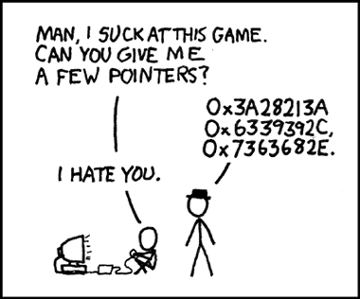
\includegraphics[width=.5\linewidth]{./gfx/xkcd-pointers}
\caption[Pointer im echten Leben]{Pointer im echten Leben. Quelle: \url{https://xkcd.com/138/}}
\end{center}
\end{figure}
\FloatBarrier

\begin{plusbox}
Während C++ ebenfalls Pointer zur Verfügung stellt, die sich dort genauso verhalten wie in der Sprache C, gilt das Paradigma, in C++ \emph{keine} Pointer zu verwenden. C++ kennt andere Konzepte, die Pointer ersetzen (bzw. verstecken) und die helfen, häufige Fehler bei der Arbeit mit Pointern zu vermeiden. Im Rahmen dieses Kurses können leider nur Stichworte genannt werden; sehen Sie dies als Motivation, einen C++-Kurs zu besuchen.

Auch wenn C++-Code \idR keine Verwendung von Pointern macht ist die Kenntnis des Konzepts auch dort sehr wichtig, da der gesamte \enquote{Unterbau} der Sprache auf den hier präsentierten Techniken beruht.
\end{plusbox}

\section{Bitweise Logik und Bit-Shifting} \label{sec:BitwiseOperator}
Für Elektronik-Anwendungen ist es oft nötig, einzelne Schalter an- oder auszuschalten. Meist geschieht dies über eine Zustandsvariable, die an einen \emph{Port} (ein Anschluss, über den Daten fließen können) gesendet wird. Diese Zustandsvariable ist dann \idR eine Ganzzahl-Variable, in der jedes Bit für einen eigenen Schalter steht. Wir benötigen also Mittel, um einzelne Bits zu manipulieren.

Dazu stehen uns die Operatoren \texttt{\~}, \texttt{\&}, \texttt{|}, \texttt{\^}, \texttt{<{}<} und \texttt{>{}>} zur Verfügung.

Die \emph{bitweise Negation} (NOT, auch \emph{1er Komplement} genannt) \texttt{\~} kehrt jedes Bit um. Betrachten wir die vorzeichenlose 8-Bit-Zahl \texttt{42} (\texttt{00101010}). Das Ergebnis der Negation ist der Wert \texttt{213} (Binärzahl \texttt{11010101}). Als Code lässt sich das wie folgt umsetzen:
\begin{codebox}[Beispiel: Bitweise Negation]
\begin{minted}[linenos]{c}
int main () {
   unsigned char source = 42;
   unsigned char result = ~source;
}
\end{minted}
\end{codebox}

Das \emph{bitweise und} (AND) \texttt{\&} vergleicht die Bits von zwei Werten und setzt das Bit im Ergebnis nur, wenn beide Bits in den Vergleichswerten gesetzt waren (\ie den Wert 1 hatten).

Beim \emph{bitweisen oder} (OR) \texttt{|} werden ebenfalls die Bits von zwei Werten verglichen. Das entsprechende Bit im Ergebnis wird jedoch bereits gesetzt, wenn mindestens eines der Vergleichsbits gesetzt war.

Das \emph{bitweise ausschließliche oder} (XOR) \texttt{\^} arbeitet genauso wie das OR, setzt das Ergebnis-Bit jedoch nur, wenn \emph{genau} eines der Vergleichsbits gesetzt war.

All dies lässt sich in den folgenden Wahrheits-Tabellen ausdrücken:
\begin{codebox}[Wahrheitstabellen: Bitweise Operatoren]
\begin{minted}{text}
     1 1 0 0   12       1 1 0 0   12       1 1 0 0   12
     1 0 1 0   10       1 0 1 0   10       1 0 1 0   10
     - AND -   --       -- OR -   --       - XOR -   --
     1 0 0 0    8       1 1 1 0   14       0 1 1 0    6
\end{minted}
\end{codebox}

Als Code lässt sich das wie folgt umsetzen:
\begin{codebox}[Beispiel: Bitweise Operatoren]
\begin{minted}[linenos]{c}
int main () {
   unsigned char lhs = 12, rhs = 10,
                 and, or, xor;
   and = lhs & rhs;    // =  8
   or  = lhs | rhs;    // = 14
   xor = lhs ^ rhs;    // =  6
}
\end{minted}
\end{codebox}

Die Negation benötigt nur ein \emph{Argument} (Wert, mit dem gearbeitet wird), und wird daher \emph{unärer Operator} genannt. Für AND, OR und XOR sind zwei Werte nötig, weswegen diese als \emph{binäre Operatoren} bezeichnet werden. Die Argumente können auch komplexe Ausdrücke sein, also Ergebnisse von Berechnungen:
\begin{codebox}[Beispiel: Bitweise Operatoren]
\begin{minted}[linenos]{c}
int main () {
   unsigned char result = ~(2 + 7 * (18 & 5));
}
\end{minted}
\end{codebox}

Bitmuster können als ganzes nach links oder rechts verschoben werden. Hierzu dienen die Operatoren \texttt{<{}<} und \texttt{>{}>}.
\begin{codebox}[Beispiel: Bitweise Operatoren]
\begin{minted}[linenos]{c}
int main () {
   unsigned char toLeft  = 170 << 1;
   unsigned char toRight =  85 >> 1;
}
\end{minted}
\end{codebox}
Dies löst folgende Veränderung aus:
\begin{codebox}[Bitshift nach links bzw. nach rechts um jeweils eine Stelle]
\begin{minted}{text}
     1 0 1 0 1 0 1 0   170       0 1 0 1 0 1 0 1    85
     ----- << 1 ----   ---       ----- >> 1 ----   ---
     0 1 0 1 0 1 0 0    84       0 0 1 0 1 0 1 0    42
\end{minted}
\end{codebox}
Bei einem Bitshift nach links werden die Bits am rechten Ende des Bitmusters mit nullen aufgefüllt.
%Stellen, die am linken Ende über die Registerbreite der aufnehmenden Variable hinaus verschoben werden, gehen verloren.
Stellen, die über das linke Ende hinaus verschoben werden, gehen verloren.
Alles eben gesagte gilt analog für den Bitshift nach rechts.

\begin{hintbox}[Multiplikation mit Zweierpotenzen]
Ein Bitshift um \texttt{n} Stellen nach links entspricht der Multiplikation mit der Zahl $2^{n}$.
Ein Bitshift um \texttt{n} Stellen nach rechts entspricht der Division durch die Zahl $2^{n}$ (Bei Ergebnissen mit Nachkommastelle wird abgerundet). Bitshifts werden schneller durchgeführt als Multiplikationen mit \texttt{*}.

Dies gilt nur für Ganzzahlen, nicht aber für Fließkommazahlen.
\end{hintbox}

\section{Typecasting} \label{sec:Casting}
Es ist gelegentlich notwendig, einen Wert von einem Datentyp in einen anderen umzuwandeln. Bei einer solchen Umwandlung kann sich das Bitmuster ändern, beispielsweise wenn die Ganzzahl \texttt{3} in die Fließkommazahl \texttt{3.0} umgewandelt wird.

Eine solche Umwandlung wird als \emph{Typecasting} bezeichnet. Die Syntax hierzu ist simpel:
\begin{codebox}[Syntax: Typecasting]
\texttt{(Ziel-Datentyp) Ausdruck}
\end{codebox}
\texttt{Ziel-Datentyp} ist ein beliebiger Datentyp, wie beispielsweise in Anhang \ref{sec:Datatypes} beschrieben. Wie üblich kann \emph{Ausdruck} ein einfacher Wert, eine Variable oder ein komplexer Ausdruck sein.

Ein Grund, den Datentyp zu ändern wurde zum Ende von Abschnitt \ref{sec:OperatorsArithmetic} bereits angeprochen: Operationen wie die Division verhalten sich unterschiedlich, abhängig davon, ob eine Fließkommazahl oder eine Ganzzahl an der Operation beteiligt ist. Solche \emph{Datentyp-spezifischen} Szenarios sind in C sehr häufig.

\begin{codebox}[Beispiel: Typecasting int zu double]
\begin{minted}[linenos]{c}
int main () {
   int x = 7, y = 5;
   double z = (double) x / y;
}
\end{minted}
\end{codebox}

\begin{hintbox}[Reihenfolge der Operationen]
Der Compiler arbeitet \enquote{von links nach rechts}, beachtet aber, dass manche Operationen \enquote{Vorrang} vor anderen haben (\eg Punkt-vor-Strich). Im obigen Beispiel wird also zuerst der Typecast der Variablen \texttt{x} durchgeführt, und dann der zum \mintinline{c}{double} konvertierte Wert von \texttt{x} durch \texttt{y} geteilt. Damit erhält \texttt{z} den Wert \texttt{1.2}.

Im folgenden Beispiel dagegen erhält \texttt{z} den Wert 1.0:
\begin{codebox}[Beispiel: Fehlerhaftes Typecasting int zu double]
\begin{minted}[linenos]{c}
int main () {
   int x = 7, y = 5;
   double z = (double) (x / y);
}
\end{minted}
\end{codebox}
Durch die Klammern interpretiert der Compiler Zeile 3 als: \enquote{Caste das Ergebnis von \texttt{x / y} zu \mintinline{c}{double}}. Da das Ergebnis von \texttt{x / y} aus der Division zweier \mintinline{c}{int}-Werte hervorgeht, wird hier gerundet und \texttt{z} erhält den (\idR falschen) Wert \texttt{1.0}.
\end{hintbox}

\section{Hierarchie der Operatoren} \label{sec:OperatorHierarchy}
Ausdrücke werden vom Compiler \enquote{von links nach rechts} ausgewertet, wobei die Vorrangigkeit mancher Operatoren beachtet wird. Die Vorrangigkeit kann Tabelle \ref{tab:OperatorPrecedence} im Anhang entnommen werden. Wo immer Unsicherheiten bestehen, kann durch Setzen von (runden Klammern) Sicherheit geschaffen werden.

\section{Zahlenformate -- Hexadezimalsystem} \label{sec:NumSystems}
Gleich zu Beginn dieses Kurses in Abschnitt \ref{sec:BinaryNumbers} haben wir das \emph{Binärsystem} (oder auch \emph{Dualsystem}) kennen gelernt, das neben dem uns vertrauten \emph{Dezimalsystem} steht\footnote{Übrigens: Das Dezimalsystem wäre völlig unbrauchbar, wenn der Mensch nicht zufällig zehn Finger hätte. (Kalenderspruch)}. Nach der dort gezeigten Idee lassen sich Zahlen in beliebigen \emph{Zahlensystemen} bzw. mit beliebiger \emph{Basis} (also Anzahl von verschiedenen Ziffern im Zahlensystem) darstellen. Von besonderer Bedeutung ist das \emph{Hexadezimalsystem} mit 16 Ziffern:

\begin{center}
\texttt{0 1 2 3 4 5 6 7 8 9 A B C D E F}
\end{center}

Um eine Zahl als \emph{hexadezimal} zu kennzeichnen wird häufig der Präfix \texttt{0x} vorangestellt. Der Ausdruck\footnote{Andere verbreitete Schreibweisen sind \texttt{10h}, \texttt{$10_{16}$} oder \texttt{$10_{hex}$}} \texttt{0x10} entspricht also der \emph{Dezimalzahl} 16. Groß- und Kleinschreibung wird hier nicht unterschieden, es gilt \texttt{0xab} = \texttt{0XAB}.

Die weiteren Informationen in diesem Abschnitt sind für besonders interessierte KursteilnehmerInnen gedacht und müssen für den Kurserfolg nicht im Detail verstanden werden. Sie werden diese Idee aber in der IT-Welt immer wieder antreffen und Nutzen aus dem Verständnis ziehen.

Die Darstellung von Zahlen bzw. allgemeiner von Bitfolgen im Hexadezimalsystem ist mitunter von Vorteil\footnote{Historische Bedeutung hat in diesem Kontext auch noch das \emph{Oktalsystem}, das die Ziffern \texttt{0..7} verwendet. Heute lebt es fast nur noch in dem Witz fort: \emph{Why do programmers confuse Halloween and Christmas? Because Oct 31 = Dec 25...}}. Wir haben bereits gehört, dass ein Computer nur Gruppen von Bits behandeln kann. Ein Byte, also eine Gruppe von 8 Bit erlaubt, wie in Abschnitt \ref{sec:Datawidth} erwähnt, 256 verschiedene Werte. Im Hexadezimalsystem wird daraus der \enquote{runde} Wert \texttt{0x100}. Ähnlich ist die Zahl der mit 16 Bit darstellbaren Zahlen gleich \texttt{0x10000} und für 32 bit erhalten wir \texttt{0x100000000} verschiedene Möglichkeiten. Dies ist kein Zufall -- Die Zahl 16 (also die Basis des Hexadezimalsystems) ist eine Potenz der Zahl 2 (also der Basis des Binärsystems). Es besteht eine \enquote{direkte Verwandschaft} zwischen Binärzahlen und Hexadezimalzahlen.

Eine Zahl, die mit $n$ Bit dargestellt wird, kann also mit $\frac{n}{4}$ Hexadezimal-Ziffern geschrieben werden. Dies ist offensichtlich praktischer als lange Ketten von 1en und 0en zu schreiben.

\begin{hintbox}[Farben als Hexadezimal-Werte]
In der Computertechnik werden Farben häufig mit \emph{Hex-Codes} beschrieben. Dies sind sechsstellige Kombinationen aus Ziffern und den Buchstaben A bis F. Tatsächlich sind diese Codes drei aneinander gereihte Hexadezimalzahlen. Diese beschreiben jeweils den Rot-, Grün- und Blau-Anteil einer Farbe. Der Dezimalwert 255 (bzw. die Hexadezimalzahl \texttt{0xFF}) beschreibt dabei \enquote{volle Intensität}, 0 (oder \texttt{0x00} dagegen sagt aus, von der Teilfarbe kommt kein Beitrag. Damit kann die Farbe Orange dann ausgedrückt werden als \texttt{0xFF7F00}: Volle Intensität Rot (\texttt{FF}), halbe Intensität Grün (\texttt{7F}) und Blau-Anteil 0 (\texttt{00}).

Siehe auch \url{https://de.wikipedia.org/wiki/Additive_Farbmischung}
\end{hintbox}

\begin{hintbox}[Zweier-Potenzen in der Computerwelt]
\emph{Alles} in der Computertechnik ist um Potenzen der Zahl 2 aufgebaut.
%Wir finden 32-bit und 64-bit-Betriebssysteme, USB-Sticks mit 2, 4, 8 oder 16 GB, oder sogar Bildschirmauflösungen wie 1024x768 Pixel.
Diese Zahlen kommen derartig häufig vor, dass sie von TechnikerInnen bereits als \enquote{runde Zahlen} wahrgenommen werden. So feierte beispielsweise Randall Munroe, Author des Webcomics \href{https://www.xkcd.com/}{xkcd} seinen eintausendsten Strip mit dieser Veröffentlichung:

\begin{center}
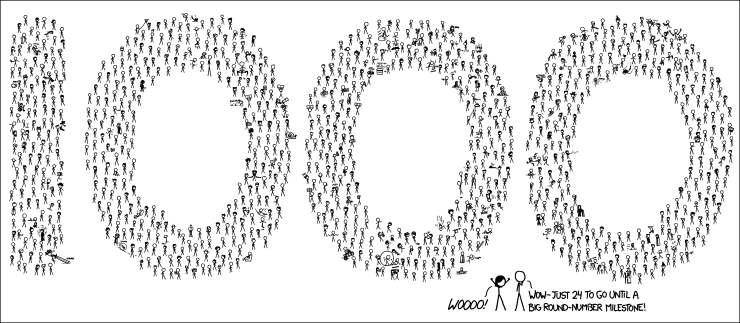
\includegraphics[width=.9\linewidth]{./gfx/xkcd-1000}
\end{center}
\captionof{figure}
	[Dezimale und binäre runde Zahlen]
	{Dezimale und binäre runde Zahlen. Quelle: \url{https://www.xkcd.com/1000/}}
\end{hintbox}

%	\include{04_Input}
%	\chapter{Conditions and Decisions} \label{chp:Conditions}
\epigraph{In any moment of decision, the best thing you can do is the right thing, the next best thing is the wrong thing, and the worst thing you can do is nothing.}{Theodore Roosevelt}

The last chapter introduced some very limited form of interactivity by introducing the possibility to enter values at runtime. We now want to extend this interactivity by breaking out of the \emph{linear flux of control}: up to now, code is executed in exactly the order the code is written, and each line of code is executed. In this chapter, we will introduce ways to break out of this restriction and learn how to tie the execution of parts of our code to \emph{conditions}.

\section{Truth Values} \label{sec:truthvalues}
To arrive at our goal of conditionally executing portions of code, we first need to learn how to formulate a condition. For this, we introduce the mathematical concept of a \emph{truth value}. A mathematical expression can either be \emph{true} or \emph{false}. For example, the expression $1 + 5 \times 8 + 1 = 42$ holds \emph{true}, while $-1 > 1$ is \emph{false}. We can use the computer to evaluate the truthfulness of any expression. For that, we introduce a new set of comparison operators:

{
	\newcolumntype{C}{>{         \centering\arraybackslash} p{.20\linewidth}}
	\newcolumntype{O}{>{\ttfamily\centering\arraybackslash} p{.25\linewidth}}
	\rowcolors{1}{white}{tabhighlight}
\begin{tabularx}
	{\linewidth}
	{CO|CO}
\toprule[1.5pt]

	\textbf{Comparison}     & \normalfont \textbf{Operator Symbol}  &
	\textbf{Comparison}     & \normalfont \textbf{Operator Symbol}
\tabcrlf

	Equality       & ==   &  Inequality         & != \\
	Less than      & <    &  Greater than       & >  \\
	Less or equal  & <=   &  Greater or equal   & >= \\

\bottomrule[1.5pt]
\end{tabularx}
\captionof{table}{Comparison operators in C}\label{tab:OperatorsComparison}
}

Note that for equality, we use a \emph{double equals sign} to distinguish this comparison operation from the value assignment.

This notion of \emph{true} or \emph{false} can be represented with a single bit. But as you know from the last chapter, a processor can ever only handle byte sized chunks of bits. So, in this context, the wasteful approach was used: \emph{false} is represented by the value \inC{0} while any \emph{nonzero} value will be seen as \emph{true}.

With these new operators, we can translate our mathematical expressions into code. They evaluate to an \inC{int}, with which we can perform any operation that we already know. For example, the expression
\begin{center}
\inC{1 + 5 * 8 + 1 == 42}
\end{center}
is a somewhat convoluted way of computing the value \inC{1}.

Since comparisons are simply \inC{int} expressions, we can do computations with them, just like with \enquote{regular maths} expressions, including storing these results in \inC{int} variables:
\begin{codebox}[truthValues.c]
\begin{minted}[linenos]{c}
#include <stdio.h>

int main () {
    int x     = 17;
    int truth = (x > 5) + (x < 5) + (x == 17);

    printf("%d true expressions.\n", truth);
}
\end{minted}
\captionof{code}{Storing turth values}
\end{codebox}

\begin{cmdbox}[Output: truthValues.c]
\begin{minted}{text}
2 true expressions.
\end{minted}
\end{cmdbox}

In this example, the three parentheses are evaluated one after another, yielding \inC{1} for \texttt{x > 5}, \inC{0} for \texttt{x < 5} and \inC{1} for \texttt{x == 17}. The three subexpressions are then summed up to give the result \inC{2}.

This is actually a thing we rarely ever do; but understanding helps us develloping a deep understanding how decision making works in a computer.

\begin{warnbox}[Symbols \texttt{true} and \texttt{false}]
In principle, you are free to use variables named \texttt{true} or \emph{false}. However, I strongly recommend against it. There are plenty of libraries (extensions to the C language) that define these symbols to mean \inC{1} or \inC{0}, respectively. They do so because expressions like \texttt{motorIsTurnedOn() == true} are just easier on human eyes than \texttt{motorIsTurnedOn() == 1}.

Defining the symbols to be constants with exactly these values is so common that when programmers see a piece of code with either of these symbols in it, they don't look up the definition, but simply assume that the symbols \emph{abide by the convention}. Going against this convention is a great way of confusing and annoying fellow coders.

While C does allow you to assign any value to the symbols \texttt{true} and \texttt{false}, most other programming languages don't. In C++, C\#, Java, Groovy and Python\footnote{In Python, the symbols actually are \texttt{True} and \texttt{False}, with a captial as a first letter. Still, The two words have a very strict definition in the programming community.}, they are \emph{reserved keywords}, \ie they are hard coded into the language itself. This is just one more reason not to adapt an unhealthy habit.
\end{warnbox}

\section{Conditional Execution of Code: \inC{if}}
\subsection{Simple \inC{if}}
Now that we know how to give answers to yes/no questions, we can tie portions of code to these answers. The keyword \inC{if} introduces an if...then block: \emph{if} some condition holds true, \emph{then} do things. In it's simplest form, this can be achieved with the following syntax:

\begin{codebox}[Syntax: Simple \texttt{if} block]
\begin{minted}{c}
if (condition) {
    statements
}
\end{minted}
\end{codebox}

In this, \texttt{condition} is anything that can be evaluated to a truth value. Usually, it is a comparison like \inC{x > 5}; but since truth values are essentially only numbers, any expression that evaluates to a number may be put here.

\texttt{statements} is one or several lines of code, \eg value assignments (\inC{x = 7 + y;}) or calls to functions (\inC{printf("hello world\n");}. These lines are executed as normal, but \emph{only if} \texttt{condition} \emph{is true}. Otherwise, they are skipped over, and the lines after the \inC{if} block are executed, \ie the lines after the closing curly brace \texttt{\}}.

Let's look at an example:
\begin{codebox}[evenNumbers.c]
\begin{minted}[linenos]{c}
#include <stdio.h>

int main () {
    int foobar = 0;

    printf("Please enter an integer: ");
    scanf("%d", &foobar);

    if (foobar % 2 == 0) {
        printf("%d is an even number.\n", foobar);
    }

    printf("You entered %d.\n", foobar);
}
\end{minted}
\captionof{code}{Detecting and handling even numbers}
\end{codebox}

\begin{tcbraster}[raster columns=2,
                  raster equal height,
                  nobeforeafter,
                  raster column skip=0.2cm]
\begin{cmdbox}[Possible Output: evenNumbers.c]
\begin{minted}{text}
Please enter an integer: 5
You entered 5.
\end{minted}
\end{cmdbox}
%
\begin{cmdbox}[Possible Output: evenNumbers.c]
\begin{minted}{text}
Please enter an integer: 4
4 is an even number.
You entered 4.
\end{minted}
\end{cmdbox}
\end{tcbraster}

First we remember that the modulus operator \texttt{\%} computes the remainder of a division. If divided by 2, even numbers will have a remainder of zero, otherwise they will have a remainder of 1. So, in line 9 we really do ask whether the value of \texttt{foobar} is even. If and only if this is the case, we execute line 10. Otherwise, we jump ahead to the end of the \inC{if} block. The block began with the opening curly brace \texttt{\{} in line 9, and ends with its closing counterpart \texttt{\}} in line 11. The code outside of the \inC{if} block is always executed, regardless of the truth value.

\begin{warnbox}[Pet Peeve: \texttt{if} \enquote{loops}]
When discussing programming with beginners, I often hear the expression \inC{if} \emph{loops}. Please internalize that this wording is \emph{simply and completely wrong}. There is no such thing as \inC{if} \emph{loops}.

A loop is a structure that we'll discuss in detail in chapter \ref{chp:loops} and that allows to jump back in the code and execute the same code several times over. So, the \enquote{trajectory} through the code looks like a loop. Loops share a syntactical similarity with \inC{if} \emph{blocks} in that the looped part is enclosed in braces and initiated by a statement that comprises of a condition; this superficial similarity, however, is the only thing linking \inC{if} \emph{blocks} to loops.

So please, for the love of ones and zeros, do not even start using this abomination of an expression, and rather refer to the structure we're discussing in this chapter as an \inC{if} \emph{block}, or simply an \inC{if} statement.
\end{warnbox}



\begin{warnbox}[Common mistake: Comparison operator \texttt{==} vs. assignment operator \texttt{=}]
It is not uncommon to put an assignment (\texttt{=}) in lieu of a comparision in the condition of an \inC{if} block. \emph{Syntactically}, this makes sense: an assignment does have a return value that usually also is a valid truth value. \emph{Semantically}, it is in by far the most cases wrong -- assigning a value within an \inC{if} condition is hardly ever what we want. At best, it is a sign of bad style. At worst, it is plain wrong and produces a hard to find bug. For that reason, let's see how this bug looks like and how to spot it:
%\end{warnbox}
%%
%\begin{warnbox}[]

\begin{warnbox}[accidentalAssignment.c, leftupper=7mm]
\begin{minted}[linenos]{c}
#include <stdio.h>

int main () {
   unsigned int rowCount = 0;
   printf("Number of rows:\n");
   scanf("%u", &rowCount);

   if (rowCount = 0) {
      printf("Error: cannot create empty table\n");
   }

   printf("Length of table: %d\n", rowCount);
}
\end{minted}
\captionof{code}{accidental assignment in an \texttt{if} block}
\end{warnbox}

This produces the following behaviour:

\begin{cmdbox}[Possible output: accidentalAssignment.c]
\begin{minted}{text}
Number of rows:
5
Length of table: 0
\end{minted}
\end{cmdbox}

As mentioned before, line 8 does not compare \texttt{rowCount} to \inC{0} but assigns the value to the variable. The \emph{return value} of this assignment is the assigned value -- \ie the value \inC{0}, which in the context of the \inC{if} block becomes the truth value \emph{false}. Consequently, we do not see the message \texttt{Error: cannot create empty table}, but find an inconsistent state in line 12.

If you use the compiler flag \texttt{-Wall}, you will see a warning on compilation:

\begin{cmdbox}[Compilerwarnung: accidentalAssignment.c]
\begin{minted}{text}
accidentalAssignment.c: In function ‘main’:
accidentalAssignment.c:9:8: warning: suggest parentheses around assignment 
    used as truth value [-Wparentheses]
    if (rowCount = 0) {
        ^~~~~~~~
\end{minted}
\end{cmdbox}
\end{warnbox}

\begin{hintbox}[Style: Indention and position of braces]
I hope you noticed that I indented the code in the \inC{if} blocks, \ie I put additional four white spaces before the instruction in the \inC{if} block. We are currently only looking at very short codes of negligible complexity, so we could do without these indentations. We will, however, soon get to a level where this extra visual clue to the \emph{structure of our code} becomes an indespensable tool for our devellopment activities. So I want to double down on the fact \emph{that} you should make indentations whenever you open a block statement -- like \inC{if} -- and remove the indentation at the end of a block.

As to \emph{how} you make these indentations, there is no fixed rule that all programmers agree to and abide by. The number of whitespaces per indentation level varies from one through eight, and some prefer tabs instead of whitespaces. Likewise, some coders prefer putting the opening brace in the same line as the statement that \enquote{causes} the block (as I do), while others rather put the opening brace in a line of its own right. There are merits to both options. Some programmers like to advertise their style with almost religious zeal, and discussions can become very emotional, as shown in figure \ref{fig:IndentStyle}.

Whatever your preference in style may be, I will ask you to abide by these rules at the very least:
\begin{itemize}
\item Do make indentations to provide visual clues for the structure of your code
\item Keep your code uniform in look by maintaining the same kind of indentation per level and same position of braces (end of line or own line) for an entire project
\item Never change the indentation style of your colleagues
\end{itemize}
\end{hintbox}

\begin{figure}
	\href{http://www.sandraandwoo.com/2015/04/13/0674-there-are-10-types-of-programmers/}{
		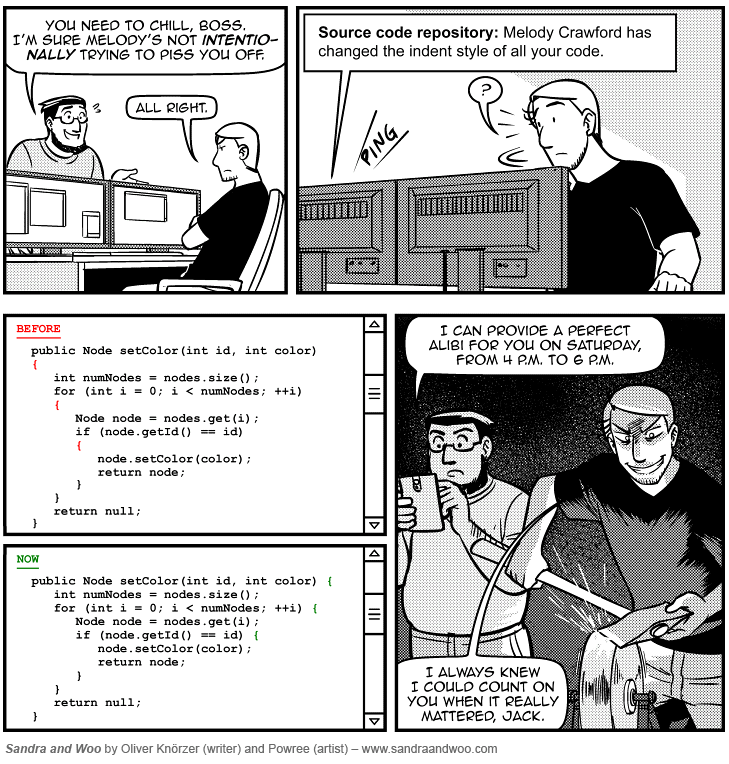
\includegraphics[width=\linewidth]{./gfx/SW-indent-style}
	}
	\caption{A realistic scenario} \label{fig:IndentStyle}
\end{figure}

If there is only a single line of code that should be tied to the condition, then the \texttt{\{}curly braces\texttt{\}} can be ommitted. The above example can thus also be shortened to:
\begin{codebox}[evenNumbers.c]
\begin{minted}[linenos]{c}
#include <stdio.h>

int main () {
    int foobar = 0;

    printf("Please enter an integer: ");
    scanf("%d", &foobar);

    if (foobar % 2 == 0)
        printf("%d is an even number.\n", foobar);

    printf("You entered %d.\n", foobar);
}
\end{minted}
\captionof{code}{Detecting and handling even numbers}
\end{codebox}

You may think of not having to type braces for one line \inC{if} blocks as a useful addition to the language. However, I strongly advise you against omitting braces, even in case of one line blocks. The reason for this advice is that it is not uncommon to amend code after it's written. If you do add lines of code to an \inC{if} block, you will have to remember adding the braces as well -- which you are very likely to forget. Even worse, the indentation that is supposed to help us to grasp the outline of our project will even conceal the error by guiding the eye and suggesting that the code has braces where there are none.

Regard this code listing \ref{code:missingBraces}:
\begin{warnbox}[missingBraces.c, leftupper=7mm]
\begin{minted}[linenos]{c}
#include <stdio.h>

int main () {
    int foo = 0;

    printf("Please enter an integer:\n");
    scanf("%d", &foo);

    if (foo % 2 == 0)
        printf("%d is an even number.\n", foo);
        printf("%d is divisible by 2.\n", foo);

    printf("You entered %d.\n", foo);
}
\end{minted}
\captionof{code}{Incorrect \texttt{if} block (missing braces)} \label{code:missingBraces}
\end{warnbox}

As intended, line 10 is only executed if \texttt{foo} is even; line 11 on the other hand will \emph{always} be executed (like lin 13), regardless of the parity of \texttt{foo}. The indentation however, suggests that it, too, is tied to the condition in line 9.

If you add the braces as soon as you type \inC{if} you cant forget it when you later edit and amend the compound statement:
\begin{codebox}[correctedBraces.c]
\begin{minted}[linenos,firstnumber=9]{c}
    if (foo % 2 == 0) {
        printf("%d is an even number.\n", foo);
        printf("%d is divisible by 2.\n", foo);
    }
\end{minted}
\captionof{code}{Corrected \texttt{if} block (added braces)}
\end{codebox}



\subsection{\inC{if}-\inC{else}}
We can expand the syntax of \inC{if} blocks by an \inC{else} clause. As you'd expect, the statements in this block are executed only if the condition in the \inC{if} condition is \emph{not} satisfied.

\begin{codebox}[Syntax: \texttt{if}-\texttt{else} block]
\begin{minted}{c}
if (condition) {
    statements_true
} else {
    statements_false
}
\end{minted}
\end{codebox}

In a full code example, this could look like so:
\begin{codebox}[ifElse.c]
\begin{minted}[linenos]{c}
#include <stdio.h>

int main () {
    int foo = 0;
  
    printf("Please enter an integer:\n");
    scanf("%d", &foo);

    if (foo % 2 == 0) {
        printf("%d is an even number.\n", foo);
    } else {
        printf("%d is an odd number.\n", foo);
    }
}
\end{minted}
\captionof{code}{\texttt{if}-{else} Blocks}
\end{codebox}

\begin{hintbox}[Bare numbers as conditions (1)]
We've learned that truth values are actually only numbers in special disguise. So whenever we test whether some expression evaluates to zero, we can omit the comparison operator, thereby creating marginally faster code, since the computer has to do one less computation step (computing the truth value). In that sense, we can re-write the former example:

\begin{codebox}[ifElseImplicitComparison.c]
\begin{minted}[linenos, firstnumber=7]{c}
    // ...
    
    if (foo % 2) {
        printf("%d is an odd number.\n", foo);
    } else {
        printf("%d is an even number.\n", foo);
    }
}
\end{minted}
\captionof{code}{\texttt{if}-{else} without explicit comparison}
\end{codebox}

We removed the \texttt{== 0} from line 9. Note that this also required flipping the true- and false case: \texttt{foo \% 2} is true when \texttt{foo} is odd, while \texttt{foo \% 2 == 0} was true when \texttt{foo} is even.
\end{hintbox}

You can nest \inC{if} blocks to almost arbitrary depth
\footnote{According to the C standard, \ie the rules according to which a C compiler has to be programmed, at least 127 levels of nested \texttt{if}s must be supported by the compiler (cf. \url{https://www.open-std.org/JTC1/SC22/WG14/www/docs/n2310.pdf}. The gcc seems to only give an error message if you nest 6200 levels (cf. \url{https://stackoverflow.com/questions/764307/what-limits-the-number-of-nested-loops-in-c}), which should be way beyond any limit of practicality.}.
Hence, we can also implement sub-conditions, that are only evaluated if a primary condition was satisfied. In the following example, we test the parity of numbers again, but limit ourselves to positive numbers:

\begin{codebox}[ifElseNested.c]
\begin{minted}[linenos]{c}
#include <stdio.h>

int main () {
    int foo = 0;
  
    printf("Please enter a positive integer:\n");
    scanf("%d", &foo);

    if (foo > 0) {
        if (foo % 2 == 0) {
            printf("%d is an even number.\n", foo);
        } else {
            printf("%d is an odd number.\n", foo);
        }
    } else {
        printf("%d is an invalid number.\n", foo);
    }
}
\end{minted}
\captionof{code}{Nested \texttt{if}-{else}}
\end{codebox}

Compare this to a -- syntactically valid -- version of the code without any indentations, and you will see why I put so much stress on the value of clear indentation:

\begin{warnbox}[ifElseNestedNotIndented.c, leftupper=7mm]
\begin{minted}[linenos]{c}
#include <stdio.h>
int main () {
int foo = 0;  
printf("Please enter a positive integer:\n");
scanf("%d", &foo);
if (foo > 0) {
if (foo % 2 == 0) {
printf("%d is an even number.\n", foo);
} else {
printf("%d is an odd number.\n", foo);
}} else {
printf("%d is an invalid number.\n", foo);
}}
\end{minted}
\captionof{code}{Nested \texttt{if}-{else} without indentations}
\end{warnbox}


\subsection{More than two cases in one \inC{if} block}
Sometimes we need to identify one of more than cases and act accordingly. If so, nested \inC{if}s are a viable means. In such a scenario, we can combine \inC{else} with a subsequent \inC{if} into a new structure\footnote{Technically, this is an application of the rule that one-line statements need no braces around them: \inC{if (condition_2) {statements}} is a one-line statement, even if \texttt{statements} takes up multiple lines. The braces bundle them together in one compound statement. Technically... \url{https://xkcd.com/1475/}}.:

\begin{codebox}[Syntax: Multi-case \texttt{if}-\texttt{else} block]
\begin{minted}{c}
if (condition_1) {
    statements_1
} else if (condition_2) {
    statements_2
} else if /* ... arbitrarily many else if blocks ... */ {
    statements_n
} else {
    statements_else
}
\end{minted}
\end{codebox}

In this form, we first evaluate \texttt{condition\_1}. If it is satisfied, the computer executes \texttt{statements\_1} and then jumps right to the end of the entire structure, \ie after the \texttt{else}, even if there are other conditions that would be met.

We can illustrate how this works in an example:

\begin{codebox}[ifMultiCase.c]
\begin{minted}[linenos]{c}
#include <stdio.h>

int main () {
    int playerCount = -1;
    printf("How many players are there?\n");
    scanf("%d", &playerCount);

    if      (playerCount < 3) {printf("That's too few players.\n")}
    else if (playerCount > 8) {printf("That's too many players.\n")}
    else                      {printf("Great! Here are the rules: ...\n");}
}
\end{minted}
\captionof{code}{Multiple cases in an \texttt{if} block}
\end{codebox}

Here you see some code that does not perform as naively expected:
\begin{warnbox}[inaccessibleCode.c, leftupper=7mm]
\begin{minted}[linenos]{c}
#include <stdio.h>

int main () {
   int foo = 0;

   printf("Please enter an integer:\n");
   scanf("%d", &foo);

   if        (foo >  5) {
      printf("%d is greater than five.\n", foo);
   } else if (foo > 10) {
      printf("This line will never be printed on screen.\n");
   } else {
      printf("%d is less than five..\n" , foo);
   }
}
\end{minted}
\captionof{code}{inaccessible code in a multi-case \inC{if} structure}
\end{warnbox}

\begin{cmdbox}[Possible Output: inaccessibleCode.c]
\begin{minted}{text}
Please enter an integer
50
50 is greater than five.
\end{minted}
\end{cmdbox}

The condition in line 11 is only ever evaluated, if the one in line 9 was already false. If the first condition \texttt{foo > 5} was true, then after printing \texttt{\%d is greater than five.}, code execution jumps right down to line 16, \ie the end of the code in this example.

\begin{defbox}[Flux of Control]
Lines 9-15 of the above code can be visualized in this flowchart:
\begin{center}
\begin{tikzpicture}
	[
		startstop/.style={rectangle, rounded corners, minimum width=3cm, minimum height=1cm,text centered, draw=black, fill=green!30!blue!30},
		decision/.style={diamond, minimum width=3cm, minimum height=1cm, text centered, draw=black, fill=violet!30},
		process/.style={rectangle, minimum width=4.5cm, minimum height=1cm, text centered, draw=black, fill=yellow!30},
		arrow/.style={thick,->,>=stealth}
	]
	
	\node (enter) at (0, 9) [startstop] {line 7 (\emph{before} \texttt{if})};
	
	\node (cond1) at (0, 6) [decision]  {\texttt{foo > 5}?};
	\node (cond2) at (0, 3) [decision]  {\texttt{foo > 10}?};
	
	\node (if_1) [process] at (5, 6) {line 10 (\enquote{greater than five})};
	\node (if_2) [process] at (5, 3) {line 12 (\enquote{greater than ten})};
	\node (else) [process] at (5, 0) {line 14 (\enquote{less than five})};
	
	\node (eif_1) at (8, 6) {};
	\node (eif_2) at (8, 3) {};
	\node (eelse) at (8, 0) {};
	
	\node (leave) at (8, -2) [startstop] {line 16 (\emph{after} \texttt{if})};
	
	\draw [arrow] (enter)  -- (cond1);
		
	\draw [arrow] 
		(cond1) -- 
		node [text width=1.2cm, midway, align=center] 
			{\color{green!70!black} yes \\ \phantom{.}}
		(if_1);
	
	\draw [arrow] 
		(cond1) -- 
		node [text width=1.2cm, midway, align=left] 
			{\color{red!70!black} no}
		(cond2);
		
	\draw [arrow] 
		(cond2) -- 
		node [text width=1.2cm, midway, align=center] 
			{\color{green!70!black} yes \\ \phantom{.}}
		(if_2);
	
	\draw [arrow] 
		(cond2) |- 
		node [text width=1.2cm, midway, align=left] 
			{\color{red!70!black} no}
		(else);
	
	\draw [arrow] (if_1) -| (leave);
	\draw [arrow] (if_2) -- (eif_2);
	\draw [arrow] (else) -- (eelse);
	\draw [arrow] (eif_1) -- (leave);
\end{tikzpicture}
\end{center}
\captionof{figure}{Flux of control in an \texttt{if}..\texttt{else if} block}

\vspace{3pt}
There is no logically possible path leading to \emph{line 12}, because it would have to pass through \texttt{foo > 5} with \emph{no} and through \texttt{foo > 10} with \emph{yes}.
\end{defbox}


\section{Logical Operators} \label{sec:OperatorsLogical}
Sometimes, execution of a piece of code should depend on more than one condition. For example, before writing a file, it has to be made sure that enough storage space is availabe \emph{and} that the filename is valid. We could achive this by nesting \inC{if} statements:

\begin{codebox}[andNested.c]
\begin{minted}[linenos, firstnumber=420]{c}
    // ...
    
    if (availableDiskSpace < 1024) {
        if (countOfInvalidCharactersInFilename > 0) {
            printf("Error: Could not write file!\n");
        }
    }
    
    // ...
\end{minted}
\captionof{code}{Nested \inC{if} to realize a logical and}
\end{codebox}

But I am pretty sure, you already noticed that we could also collapse this into a single \inC{if} statement by using the \emph{and} operation from the previous chapter. A comparison like \texttt{<} or \texttt{>} produces an integer, which is either 1 or zero. We can join several ones and zeros with the bitwise operators \texttt{\&}, \texttt{|} and \texttt{\textasciicircum}. Thus, the same result is achieved by this code:
\begin{codebox}[andBitwise.c]
\begin{minted}[linenos, firstnumber=420]{c}
    // ...
    
    if ((availableDiskSpace < 1024) & (countOfInvalidCharactersInFilename > 0)) {
        printf("Error: Could not write file!\n");
    }
    
    // ...
}
\end{minted}
\captionof{code}{Bitwise operator joins two conditions in an \inC{if} statement} \label{code:bitwiseAndIf}
\end{codebox}

For reasons I will explain in the next few paragraphs, in such a situation we would prefer \emph{logical operators} over \emph{bitwise operators}. Each of the bitwise operators (\emph{and}, \emph{or}, \emph{xor} and \emph{not}) has a logical counterpart. Both kinds of operators perform the same principle operations; \emph{true and true} will always give \emph{true}, no matter whether you perform a bitwise or a logical \emph{and}. The primary difference between the two is that the logical operators first reduce their operands to \emph{booleans}, i.e. to a single true/false value.

The \emph{bitwise} and between \texttt{11 == 1011$_2$} and \texttt{7 == 0111$_2$} is \texttt{3 == 0011$_2$}. The \emph{logical} and, on the other hand, is simply \texttt{1} or \emph{true}, because both operands \texttt{11} and \texttt{7} are nonzero and therefore count as \emph{true}. Table \ref{tab:logicalAndBitwiseOperators} shows which symbols are used for which operation:

{
\newcolumntype{N}{>{         \centering\arraybackslash} p{.15\linewidth}}
\newcolumntype{R}{>{\ttfamily\centering\arraybackslash} p{.25\linewidth}}
\begin{center}
\rowcolors{1}{white}{tabhighlight}
\begin{tabularx}
	{.73\linewidth}
	{NRR}
\toprule[1.5pt]

    \textbf{Operation} & \textrm{\textbf{Bitwise Operator}}  &  \textrm{\textbf{Logical Operator}}
\tabcrlf
    and &               \& & \&\& \\
    or  &               |  & ||   \\
    xor & \textasciicircum & !=   \\
    not & \textasciitilde  & !    \\

\bottomrule[1.5pt]
\end{tabularx}
\end{center}
\captionof{table}{Logical and bitwise operators in C}\label{tab:logicalAndBitwiseOperators}
}

Note that it is not a mistake to put the inequality operator \texttt{!=} in the table as the logical xor operator. If you compare to the behaviour listed in table \ref{tab:booleanLogic}, you will find that \emph{inequality} is exactly what a logical xor tests for.

So, why should we write
\mint{c}{if ((availableDiskSpace < 1024) && (countOfInvalidCharactersInFilename > 0))}
instead of using a bitwise operator like in code listing \ref{code:bitwiseAndIf}?

In day-to-day life, the principal reason is semantics: using a logical operator says that we really only care about yes-or-no information; bitwise operators on the other hand imply that some black magic on individual bits is happening\footnote{which usually makes experienced coders nervous}. They also allow treating values in themselves as truth values. Compare these two pieces of code:
{
\begin{tcbraster}[raster columns=2,
                  raster equal height,
                  nobeforeafter,
                  raster column skip=0.2cm]
\begin{codebox}[nonzeroLogicalAnd.c]
\begin{minted}[linenos, firstnumber=69]{c}
if (x && y) {
  printf("Both x and y are nonzero.");
}
\end{minted}
\end{codebox}
%
\begin{codebox}[nonzeroBitwiseAnd.c]
\begin{minted}[linenos, firstnumber=69]{c}
if ((x != 0) & (y != 0)) {
  printf("Both x and y are nonzero.");
}
\end{minted}
\end{codebox}
\end{tcbraster}
\captionof{code}{Bitwise and logical conjunction for nonzero-test}
}

The left example using the logical and works in this shortened form no matter what values \texttt{x} and \texttt{y} store. For the bitwise operators, on the other hand, an explicit comparison to zero is needed\footnote{You might still find the right hand side form easier to understand due to its explicitness, and this point of view has its merit. Of course, you can always combine both versions, \ie use logical operators with explicit comparisons.} (think of the example \texttt{x = 1} and \texttt{y = 2}. Without the explicit comparison, the bitwise \emph{and} would give \texttt{0} or false).

Another major difference is the fact that the bitwise \emph{and} and \emph{or} are \emph{short circuited}. This means that the computer tries to save some time by evaluating the second operand only when this is necessary. You know that for an \emph{and}, both operands need to be \emph{true}. If the left hand side operand is already known to be \emph{false}, we automatically know that the result of the \emph{and} will always be \emph{false}, no matter what comes to the right of it. This can be used to prevent nonsensical operations:
\begin{codebox}[Example: preventDivByZero.c]
\begin{minted}[linenos, firstnumber=69]{c}
if (x && (y / x > 5)) {
    printf("Treshold surpassed");
}
\end{minted}
\captionof{code}{Short circuiting}
\end{codebox}

We know that a division by zero is ill-defined. This also holds for programming in C: a program trying to divide by zero will usually crash\footnote{unless you are using floating point numbers... but more on that in chapter \ref{chp:misc}.}, which is obviously bad. For that reason, we should always make sure the denominator of a division is nonzero. In the above example, due to the short circuiting behavior of the logical \emph{and}, the expression \texttt{y / x} is only evaluated if \texttt{x} itself was already nonzero.

In a similar manner, the logical or (\texttt{||}) evaluates its right hand side operand only if the left hand side was \emph{false}, because \emph{true or anything} will always be \emph{true}.

\begin{hintbox}[Rule of thumb: two character operators with \texttt{if}]
We already encountered the fact that the assignment operator (\texttt{=}) is usually misplaced in an \inC{if} statement. We have seen that confusing the bitwise operators with the logical ones can have unintended consequences, too.

While it sadly does not always hold, I recommend you to adopt the rule of thumb: \emph{an \inC{if} requires a two-character operator} (\ie \texttt{==}, \texttt{\&\&}, ...). Notable exceptions from this rule are \texttt{<}, \texttt{>} and \texttt{!}, and every time you do evil bit hacking.
\end{hintbox}

\begin{hintbox}[Bare numbers as conditions (2)]
Whether or not a number is nonzero is a question we have to answer very often in programming. We've already learned that we can drop the explicit comparision to zero when the code we want to run code if some number is \emph{nonzero}. With the logical \emph{not}, we can also run code only when it is \emph{zero}:

\vspace{6pt}
\begin{codebox}[implicitIfZero.c]
\begin{minted}[linenos]{c}
#include <stdio.h>

int main () {
    unsigned int rowCount = 0;
    printf("Number of rows:\n");
    scanf("%u", &rowCount);

    if (!rowCount) {
        printf("Error: cannot create empty table\n");
    }
}
\end{minted}
\captionof{code}{logical not to test for zero values}
\end{codebox}
\end{hintbox}

In particular using the \emph{or} conjunction can help reduce redundant code. Regard the following example:
{
\begin{tcbraster}[raster columns=2,
                  raster equal height,
                  nobeforeafter,
                  raster column skip=0.2cm]
\begin{warnbox}[ifSequence.c, leftupper=7mm]
\begin{minted}[linenos]{c}
#include <stdio.h>

int main () {
    unsigned int playerCount = 0;

    printf("number of players:\n");
    scanf("%u", &playerCount);

    if (playerCount < 2) {
        printf(
            "Game not apt for %d ",
            playerCount
        );
        printf("players.\n");
    }

    if (playerCount > 5) {
        printf(
            "Game not apt for %d ",
            playerCount
        );
        printf("players.\n");
    }
}
\end{minted}
\end{warnbox}
%
\begin{codebox}[ifConjunction.c]
\begin{minted}[linenos]{c}
#include <stdio.h>

int main () {
    unsigned int playerCount = 0;

    printf("number of players:\n");
    scanf("%u", &playerCount);

    if ((playerCount < 2) ||
        (playerCount > 5)
       ) {
        printf(
            "Game not apt for %d ",
            playerCount
        );
        printf("players.\n");
    }
}
\end{minted}
\end{codebox}
\end{tcbraster}
\captionof{code}{Avoiding redundant code with logical operators}
}

Not only is the right hand side code much shorter; it is also easier to maintain and debug. If we later want do more than only print a warning that a given player number is not suitable, in the left hand code we need to edit in these changes in two places, and are therefore twice as likely to make typos or (most dangerously) can outright forget to edit the second \inC{if} statement.

\begin{hintbox}[Avoid redundant code]
Whenever you feel like copy-pasting your code, always think twice whether there is not a possibility to restructure your code such that you avoid redundancy. Experience shows that you always spend \emph{way longer} to find and fix bugs due to redundancy than it takes to refactor your code into a more maintainable form.
\end{hintbox}

\section{Many cases: \inC{switch}}


\rule{\textwidth}{2pt}
\newpage
%TODO

%exos:
% - why is 5 & 2 false?
% - which of these are equivalent ~> modus tollens; !!x and (x != 0)

\section{Fallunterscheidungen: \inC{switch}}
Das Schlüsselwort \inC{switch} wird benutzt, um Fallunterscheidungen mit vielen einzelnen Fällen umzusetzen. Die Form von \inC{switch}-Blöcken lautet:

\begin{codebox}[Syntax: \texttt{switch}]
\begin{minted}{c}
switch (Ausdruck) {
   case Wert1 :
      Anweisungen;
      break;
   case Wert2 :
      Anweisungen;
      break;
   ...
   default:
      Anweisungen;
      break;
}
\end{minted}
\end{codebox}

\texttt{Ausdruck} ist dabei ein beliebiger Ausdruck, der zu einer \emph{Ganzzahl} ausgewertet werden kann. Fließkommawerte oder andere Datentypen werden von \inC{switch} leider nicht unterstützt. Dasselbe gilt für \texttt{Wert1}, \texttt{Wert2}, \ldots; jedoch müssen diese Ausdrücke bereits zur \emph{Compile-Zeit} feststehen. Das bedeutet, dass \texttt{Wert1}, \texttt{Wert2}, \ldots keine Variablen oder Elemente enthalten dürfen, die erst bei Ausführung des Programms (zur \emph{Laufzeit}) feststehen.

Wenn die Aussage \texttt{Ausdruck == Wert1} wahr ist, wird der Code unter der entsprechenden \inC{case}-Zeile ausgeführt. Entsprechendes gilt für \texttt{Wert2}, \ldots. Gilt für keinen der angegebenen Werte Gleichheit, so werden die Anweisungen unter \inC{default} ausgeführt.

In der Anwendung kann dies so aussehen:

\begin{codebox}[Beispiel: Menü mit \texttt{switch}]
\begin{minted}[linenos]{c}
#include <stdio.h>

int main () {
   int selection = -1;

   printf("Bitte wählen Sie einen Menüpunkt:\n");
   printf("  1) Spiel starten\n");
   printf("  2) Optionen\n");
   printf("  3) Highscore zeigen\n");
   printf("  0) Beenden\n");

   scanf("%d", &selection);

   switch (selection) {
      case 1 :
         // Code für: Spiel Starten
         break;
      case 2 :
         // Code für: Optionen
         break;
      case 3 :
         // Code für: Highscore
         break;
      case 0 :
         // Code für: Beenden
         break;
      default:
         printf("Ungültige Eingabe!\n");
         break;
   }
}
\end{minted}
\end{codebox}

Der \inC{default}-Teil ist optional. Lässt man diesen weg und trifft keine der \inC{case}-Klauseln zu, so wird nichts ausgeführt -- die Ausführung des Codes wird am Ende des \inC{switch}-Blocks fortgesetzt.

Die Werte zu den \inC{case}-Klauseln dürfen im selben \inC{case}-Block nur jeweils ein einziges Mal vorkommen.

Man kann sich \inC{switch}-Blocks als Kurzform für \inC{if}-Blocks vorstellen\footnote{Die tatsächliche Umsetzung ist etwas komplexer und enthält einige Optimerungsschritte, die hier nicht besprochen werden können. Diese interne Umsetzung ist der Grund, weswegen \inC{switch} nur mit Ganzzahlen funktioniert.}. Das vorige Beispiel lässt sich auch so programmieren:

\begin{codebox}[Beispiel: Menü mit \texttt{if}]
\begin{minted}[linenos]{c}
#include <stdio.h>

int main () {
   int selection = -1;

   printf("Bitte wählen Sie einen Menüpunkt:\n");
   printf("  1) Spiel starten\n");
   printf("  2) Optionen\n");
   printf("  3) Highscore zeigen\n");
   printf("  0) Beenden\n");

   scanf("%d", &selection);

   if        (selection == 1) {
      // Code für: Spiel Starten
   } else if (selection == 2) {
      // Code für: Optionen
   } else if (selection == 3) {
      // Code für: Highscore
   } else if (selection == 0) {
      // Code für: Beenden
   } else {
      printf("Ungültige Eingabe!\n");
   }
}
\end{minted}
\end{codebox}

Wichtig ist das Schlüsselwort \inC{break}. Mit diesem Befehl wird eine Kontrollstruktur wie ein \inC{switch}-Block verlassen und die Codeausführung wird hinter dem aktuellen Block fortgesetzt. Betrachten Sie das folgende Beispiel:

\begin{warnbox}[Beispiel: \texttt{switch} ohne \texttt{break}, leftupper=7mm]
\begin{minted}[linenos]{c}
#include <stdio.h>

int main () {
   int x = 1;

   switch (x) {
      case 0 :
         printf("0\n");
      case 1 :
         printf("1\n");
      case 2 :
         printf("2\n");
      case 3 :
         printf("3\n");
      default :
         printf("d\n");
   }
}
\end{minted}
\end{warnbox}

Das Ergebnis dieses Codes ist:
\begin{cmdbox}[Ausführungsbeispiel: \texttt{switch} ohne \texttt{break}]
\begin{minted}{text}
1
2
3
d
\end{minted}
\end{cmdbox}

Wie zu erwarten springt die Ausführung mit \inC{switch} von Zeile 6 nach Zeile 9. Da hier aber keine \inC{break}s gesetzt wurden, \enquote{fällt die Ausführung durch die \inC{case}-Klauseln}. Das bedeutet, dass am Ende der \inC{case}-Klausel \texttt{1} die Code-Ausführung in Zeile 11 fortgesetzt wird, und somit alle \texttt{printf}-Anweisungen ausgeführt werden. Wird der Compiler mit der Option \texttt{-Wimplicit-fallthrough} gestartet, so finden Sie in der Compiler Ausgabe eine entsprechende Warnung:

\begin{cmdbox}[Compiler-Warnung: \texttt{switch} ohne \texttt{break}]
\begin{minted}{text}
myProgram.c: In function ‘main’:
myProgram.c:8:7: warning: this statement may fall through
[-Wimplicit-fallthrough=]
       printf("0\n");
       ^~~~~~~~~~~~~
myProgram.c:10:5: note: here
     case 1 :
     ^~~~
...
\end{minted}
\end{cmdbox}

Kontrollstrukturen wie \inC{switch} und \inC{if} können (nahezu) beliebig tief ineinander verschachtelt werden.

\section{Kombinierte Fallunterscheidung und Wertzuweisung -- der Ternäre Operator \texttt{?}}
Nicht selten soll der Wert einer Variablen von einer Bedingung abhängen. Wir kennen bisher die Form

\begin{codebox}[Beispiel: Bedingte Wertzuweisung mit \texttt{if}]
\begin{minted}[linenos]{c}
int main () {
   int Bedingung = 1, Variable;

   if (Bedingung) {
      Variable = 1;
   } else {
      Variable = 2;
   }
}
\end{minted}
\end{codebox}

Diese von einer Bedingung abhängige Wertzuweisung kann auch kompakt in einer einzelnen Zeile geschrieben werden. Mit dem \emph{ternären Operator}\footnote{von \emph{ternär}: das Dritte. Dieser Operator braucht drei \emph{Argumente}. Die Addition \texttt{+} ist beispielsweise ein \emph{binärer} Operator, da sie zwei Argumente braucht -- eben die beiden Zahlen, die addiert werden sollen.} \texttt{?} lässt sich dieser Code auch schreiben als:

\begin{codebox}[Beispiel: Bedingte Wertzuweisung mit dem ternären Operator]
\begin{minted}[linenos]{c}
int main () {
   int Bedingung = 1, Variable;

   Variable = Bedingung ? 1 : 2;
}
\end{minted}
\end{codebox}

Wie bereits bei \inC{if} ist \texttt{Bedingung} ein Ausdruck, dem ein Wahrheitswert zugeordnet werden kann. Ist \texttt{Bedingung} erfüllt, so wird der Ausdruck direkt hinter dem \texttt{?} ausgewertet und zugewiesen. Andernfalls wird der Ausdruck hinter dem \texttt{:} verwendet.

Variablen, die in \texttt{Bedingung} vorkommen, können auch in den Rückgabewerten vorkommen. So lässt sich beispielsweise die Betragsfunktion folgendermaßen implementieren:

\begin{codebox}[Beispiel: Betrag einer Zahl  mit dem ternären Operator]
\begin{minted}[linenos]{c}
int main () {
   int x = -42;

   x = x >= 0 ? x : -x;
}
\end{minted}
\end{codebox}

%	\chapter{Die CPP-Referenz am Beispiel der math-library}\label{chp:maths}
\epigraph{Do not worry about your difficulties in Mathematics. I can assure you mine are still greater.}{Albert Einstein}

Zu vielen mathematischen Problemen wie Berechnung der Wurzel oder des Sinus einer Zahl stehen in der math-library \texttt{libm}\footnote{Wie in Abschnitt \ref{sec:Compile} besprochen, muss dem Compiler mitgeteilt werden, wenn eine Bibliothek verwendet wird. Während allgemein von der \emph{math-library} gesprochen wird, heißt die einzubindende Datei leider einfach nur \texttt{m} -- ein unschöner Umstand, mit dem wir leben müssen.} Lösungen bereit. Ich möchte Sie dazu einladen, diese Funktionen selbst zu erkunden. Dazu wird uns die Befehlsreferenz unter \url{https://en.cppreference.com/w/c} dienen. In diesem Kapitel lernen Sie, sich in der Befehlsreferenz zurecht zu finden und nützliche Features selbst zu entdecken.

\section{Überblick über die Seite cppreference.com}
Wenn Sie die Seite \url{https://en.cppreference.com/w/c} besuchen, sollten Sie ein Bild wie in Abbildung \ref{fig:cpp-home} sehen.

\begin{figure}[h!]
	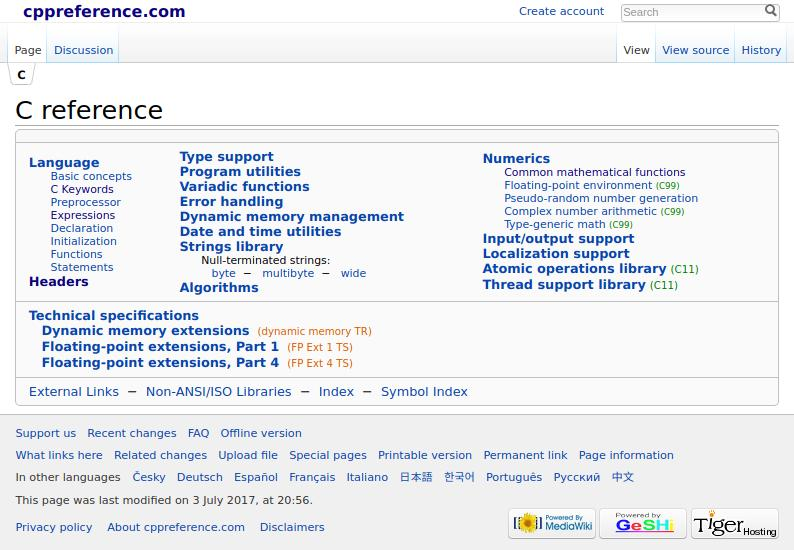
\includegraphics[width=\linewidth]{./gfx/cpp-home}
	\caption{Die Startseite der C-Referenz \url{https://en.cppreference.com/w/c}} \label{fig:cpp-home}
\end{figure}

Der angegebene Link führt Sie auf die \emph{englische} Befehlsreferenz. Übersetzungen in verschiedene andere Sprachen, darunter auch Deutsch, stehen zur Verfügung. In der Regel sind diese aber weit weniger ausführlich und oft unvollständig\footnote{Meiner Erfahrung nach gilt dies generell in der Welt des Programmierens: Nützliche Ressourcen sind oft nur in Englisch verfügbar oder nur in dieser Sprache in vollem Umfang.}. Wenn Sie dennoch mit der deutschen Version arbeiten möchten, finden Sie auf jeder Seite der Referenz am unteren Rand die Zeile \emph{In other languages} und dahinter Links, die sie zu einer entsprechenden Übersetzung führen.

Am rechten oberen Rand befindet sich eine Textbox, in die Sie einen Suchbegriff eingeben können. Die Suche liefert ihnen Ergebnisse zu ihrem Begriff sowie zu \enquote{ähnlichen Ausdrücken}. Die Ergebnisse sind in zwei Spalten sortiert und betreffen die Sprache C++ (links) bzw. C (rechts). In Abbildung \ref{fig:cpp-search} finden Sie das Ergebnis der Suche nach dem Befehl \texttt{printf}. Jede Zeile der Suchergebnisse ist ein Link auf einen Artikel, der den Befehl oder das Konzept erklärt.

\begin{figure}[h!]
	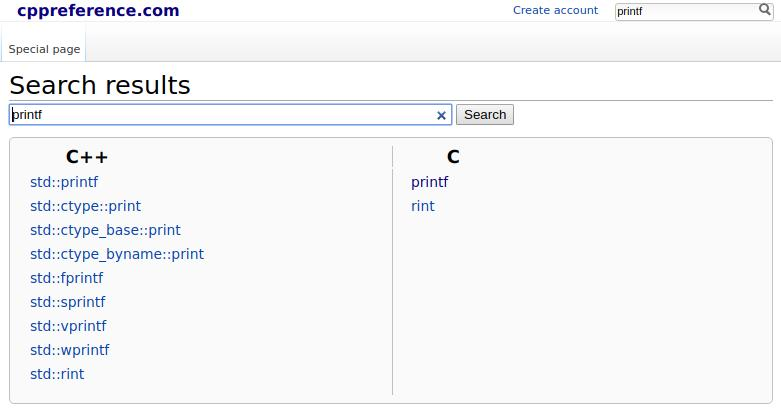
\includegraphics[width=\linewidth]{./gfx/cpp-search}
	\caption{Suchergebnisse in der CPP-Referenz} \label{fig:cpp-search}
\end{figure}

Ein solcher Artikel sieht \idR aus wie in Abbildung \ref{fig:cpp-printf}. Befehle, die sich sehr ähnlich verhalten werden teils zu einem einzelnen Artikel zusammengefasst. Nach der Überschrift finden Sie die Zeile \emph{Defined in header <stdio.h>}, die Ihnen mitteilt, welche \mintinline{c}{#include}s Sie setzen müssen, um den oder die erklärten Befehle in Ihren Programmen nutzen zu können.

Weiter schließt sich eine Syntax-Übersicht an, in der die erwarteten Parameter sowie ihre Datentypen aufgelistet werden. Manche dieser Formen standen nicht in der \enquote{Urform} der Sprache C zur Verfügung. Für solche Features, die erst mit einem bestimmten Standard eingeführt wurden ist in der Referenz in grün das Einführungsdatum bzw. das \enquote{Verfallsdatum} der Form aufgeführt. Ich erinnere Sie daran, dass wir hier den Standard C11 besprechen. In Abschnitt \ref{sec:cpp-article} werden wir anhand eines übersichtlicheren Beispiels auf die Struktur der Artikel eingehen.

\begin{figure}[h!]
	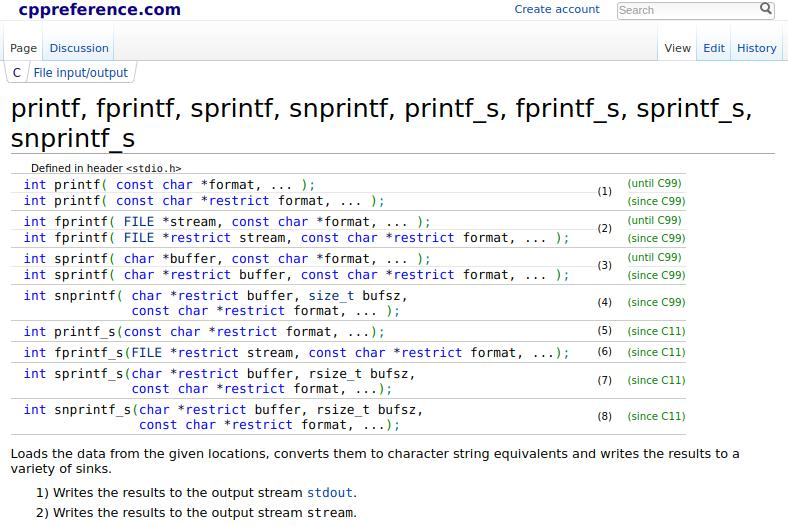
\includegraphics[width=\linewidth]{./gfx/cpp-printf}
	\caption{Anfang des Artikels zu \texttt{printf} auf der CPP-Referenz} \label{fig:cpp-printf}
\end{figure}

\section{Funktionen zu einer Aufgabe finden}
Die Funktionen, die die Sprache C zur Verfügung stellt, sind in thematisch verwandten \emph{Bibliotheken} organisiert. Zu jeder Bibliothek existiert ein \emph{Header}, dessen Name einen Hinweis auf die darin enthaltenen Funktionen gibt. Um Lösungen zu einem gegebenen Problem zu suchen, durchsucht man also am besten die Liste der Header. Diese kann von der Hauptseite aus über den Link \emph{Headers} erreicht werden (siehe Abbildung \ref{fig:cpp-home}, erste Spalte unten). Dieser Link führt Sie zu einer Ansicht wie in Abbildung \ref{fig:cpp-headers}.

\begin{figure}[h!]
	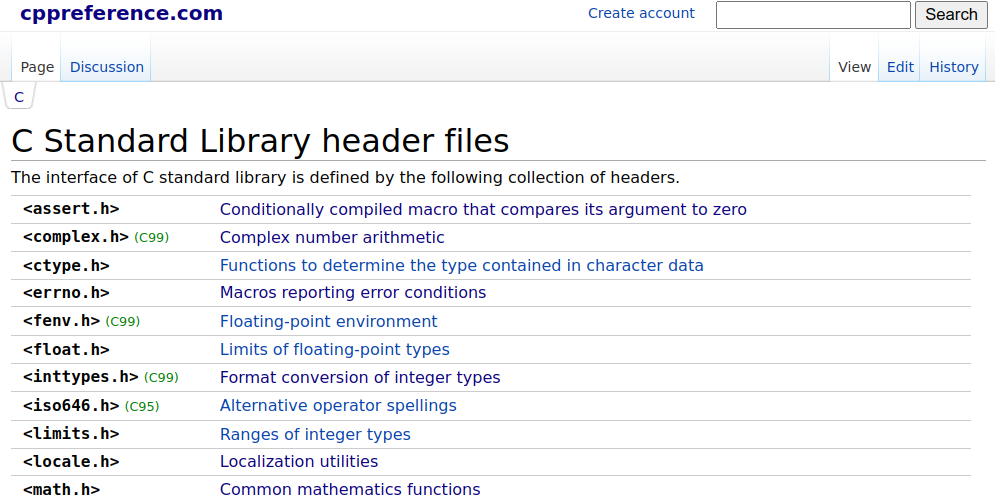
\includegraphics[width=\linewidth]{./gfx/cpp-headers}
	\caption{Liste der Header auf der CPP-Referenz} \label{fig:cpp-headers}
\end{figure}

In diesem Kapitel wollen wir uns mit mathematischen Funktionen befassen; wir klicken daher auf den Link \emph{Common mathematical functions}.

\begin{figure}[h!]
	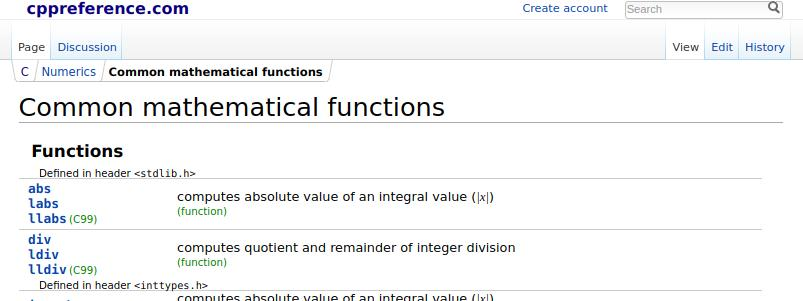
\includegraphics[width=\linewidth]{./gfx/cpp-math}
	\caption{Funktionen der math-library in der CPP-Referenz} \label{fig:cpp-math}
\end{figure}

Wie Sie in Abbildung \ref{fig:cpp-math} sehen, sind die Funktionen in einem ähnlichen Format aufgelistet wie schon die Header. Zu vielen Aufgaben stehen mehrere Funktionen zur Verfügung. Dies hat den Grund, dass die Sprache C \emph{strong-typed} ist, \ie dass Unterschiede zwischen beispielsweise \mintinline{c}{float}- und \mintinline{c}{double}-Werten bestehen. Funktionen, die mit einem \texttt{f} beginnen, berechnen \idR einen \mintinline{c}{float}-Wert; der Anfang \texttt{l} weist auf einen \mintinline{c}{long}-Wert hin und \texttt{ll} erzeugt einen \mintinline{c}{long long}-Wert. Für manche Kontexte sind Ganzzahlen unsinnig; dort weist der Suffix \texttt{l} auf \mintinline{c}{long double} hin. Ist dem Funktionsnamen kein solcher \emph{Präfix} vorangestellt, wird ein \mintinline{c}{double}-Wert berechnet\footnote{Die Benennungs-Logik der C-Standardbibliotheken folgt oft noch veralteten Konventionen, die solche kryptischen Namen hervorbringen. Moderne ProgrammiererInnen bevorzugen \enquote{klare Namen}. Damit auch ältere Code-Teile weiterhin funktionieren musste diese Benennungsregeln fortgeführt werden.}.

Aufgrund des \emph{strong typing} muss auch für die Argumente der Funktionen unterschieden werden. Hier geben die \emph{Suffixe} \texttt{f}, \texttt{l} und \texttt{ll} den Datentyp des Arguments an.

Beispielsweise finden Sie die Funktion \texttt{abs}, die den Absolutbetrag einer \mintinline{c}{double}-Zahl berechnet und als \mintinline{c}{double}-Wert zurückgibt. Daneben ist aber auch \ua die Funktion \texttt{fabsl} aufgelistet, die ebenso den Absolutbetrag einer Zahl berechnet. Die Zahl wird für diese Funktion jedoch als \mintinline{c}{long}-Wert angegeben und das Ergebnis als \mintinline{c}{float} berechnet.

\section{Der Artikel zu \texttt{sqrt}} \label{sec:cpp-article}
\begin{figure}[h!]
	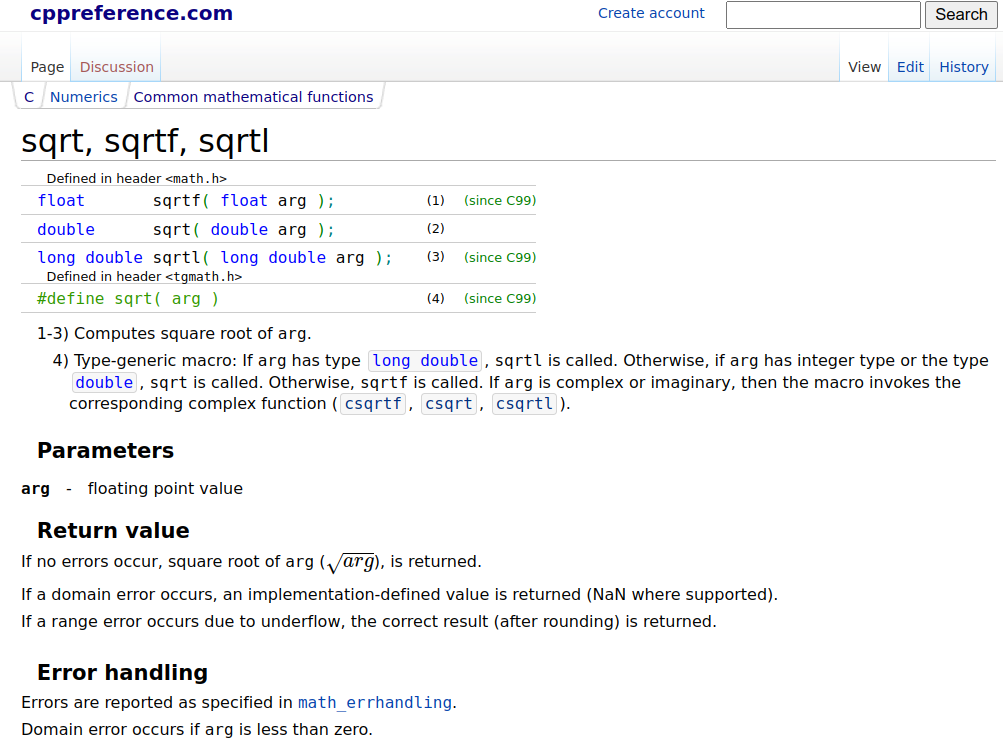
\includegraphics[width=\linewidth]{./gfx/cpp-sqrt}
	\caption{Anfang des Artikels zu \texttt{sqrt} in der CPP-Referenz} \label{fig:cpp-sqrt}
\end{figure}

Abbildung \ref{fig:cpp-sqrt} zeigt den Anfang des Artikels zum Befehl \texttt{sqrt}. Die Zeile \emph{Defined in header <math.h>} weist darauf hin, dass wir \mintinline{c}{#include <math.h>} setzen müssen, um \texttt{sqrt} benutzen zu können. Von dem Befehl stehen drei Varianten zur Verfügung, von denen zwei erst mit dem Standard C99 eingeführt wurden (Punkte 1 bis 3). Weiterhin wurde mit dem Standard C99 ein \emph{Makro} eingeführt (Punkt 4), das wir an dieser Stelle noch nicht bearbeiten wollen. In Kapitel \ref{chp:Preprocessor} besprechen wir die hierzu relevanten Techniken. Für den Moment können Sie den Punkt ignorieren\footnote{Wenn Sie später im Kursverlauf nochmals diesen Artikel in der Referenz lesen, beachten Sie bitte, dass für die Benutzung des Makros der Header \emph{<tgmath.h>} eingebunden werden muss.}.

Unter der tabellarischen Übersicht der im Artikel besprochenen Funktionen finden Sie eine Kurzbeschreibung des Effekts der einzelnen Formen. \emph{1-3) Computes square root of arg.} -- alle hier besprochenen Funktionen berechnen also die Quadratwurzel eines Arguments \texttt{arg}. Der Unterschied ist der Datentyp des Ergebnisses bzw. des Arguments.

Unter \emph{Parameters} finden Sie genauere Erläuterungen zu den Argumenten, die den Funktionen übergeben werden können. Für \texttt{sqrt} ist dies die nüchterne Erklärung, dass \texttt{arg} eine beliebige Fließkommazahl beschreibt. Bei der Funktion \texttt{printf} wird hier etwa aufgelistet, wie ein Formatstring auszusehen hat.

Funktionen berechnen einen Wert, der dann einer anderen Variablen zugewiesen werden kann. Betrachten Sie das folgende Beispiel:

\begin{codebox}[Beispiel: Betrag einer Zahl  mit dem ternären Operator]
\begin{minted}[linenos]{c}
#include <math.h>

int main () {
   double root = sqrt(81.0);
}
\end{minted}
\end{codebox}

Wir benutzen die Funktion \texttt{sqrt} um aus dem \mintinline{c}{double}-Wert \texttt{81.0} die Wurzel zu berechnen und speichern diesen Wert der Wurzel dann in der Variablen \texttt{root}. Dieser berechnete Wert wird als Rückgabewert (\emph{Return Value}) der Funktion bezeichnet.

Der Abschnitt \emph{Return Values} gibt Details zu dem berechneten Wert unter der Annahme verschiedener Szenarios.

Wenn kein Fehler auftritt, wird die Quadratwurzel von \texttt{arg} berechnet. Wie Sie wissen, existiert aber nicht zu jeder Zahl eine Quadratwurzel. So sind negative Werte für \texttt{arg} nicht zulässig -- dies ist gemeint mit \emph{If a domain error occurs}. In diesem Fall hängt das Ergebnis von der Version des Compilers ab (\emph{an implementation-defined value is returned}). In der Regel wird aber ein spezielles Bitmuster erzeugt, das sicher als \enquote{Fehler-Wert} interpretiert werden kann (\emph{NaN where supported} -- \emph{NaN} steht für \emph{Not a Number}, also ein Fehlerwert. Siehe hierzu mehr in Abschnitt \ref{sec:NAN}).

Die letzte Zeile \emph{If a range error occurs due to underflow} beschreibt das Verhalten, wenn der Wert von \texttt{arg} nicht mehr korrekt mit seinem Datentyp abgebildet werden kann (vgl. Abschnitt \ref{sec:Datatypes} im Anhang -- manche Werte sind zu groß oder haben zu viele Nachkommastellen, um beispielsweise als \mintinline{c}{double} exakt abgebildet zu werden). In diesem Fall wird mit einem gerundeten Wert gerechnet.

Unter \emph{Error Handling} werden weitere Details aufgelistet, die das Verhalten von \texttt{sqrt} in \enquote{abnormalen} Situationen beschreiben. Im Allgemeinen ist es nicht nötig, all diese Details im Kopf zu behalten -- dafür ist die Referenz da.

Am Ende der meisten Artikel finden Sie zu jedem Befehl einen Beispiel-Code, der die Anwendung der besprochenen Funktion verdeutlicht, sowie ein Ausgabebeispiel.

\section{Weitere nützliche Funktionen der math-library}
Die folgende Tabelle listet sehr gebräuchliche Funktionen sowie eine Kurzbeschreibung auf. Mit der cpp-Referenz sollten Sie nun dazu in der Lage sein, diese Funktionen in Ihren Programmen anzuwenden.

\begin{table}[h!]
	\newcolumntype{C}{>{\ttfamily\centering\arraybackslash} p{.2\linewidth}}
	\newcolumntype{D}{>{         \centering\arraybackslash} p{.7\linewidth}}
	\rowcolors{1}{white}{chameleonblue2}
\begin{center}
\begin{tabularx}
	{.95\linewidth}
	{CD}
\toprule[1pt]

	\normalfont Funktion  &  Effekt
\tabcrlf

	sqrt  & Quadratwurzel einer Zahl \\
	cbrt  & Kubikwurzel einer Zahl   \\
	pow   & Potenz einer Zahl \texttt{x} zu einem Exponenten \texttt{y}: $x^{y}$ \\
	exp   & Exponentialfunktion      \\
	log   & Natürlicher Logarithmus  \\
	sin   & Sinus                    \\
	cos   & Cosinus                  \\
	tan   & Tangens                  \\
	asin  & Arcussinus               \\
	acos  & Arcuscosinus             \\
	atan  & Arcustangens             \\
	atan2 & Arcustangens mit Unterscheidung der Quadranten \\
	ceil  & Zahl aufrunden           \\
	floor & Zahl abrunden            \\
	trunc & Nachkommaanteil abschneiden \\
	round & Zahl runden              \\

\bottomrule[1pt]
\end{tabularx}
\end{center}
\caption{Gängige Funktionen der math-library}\label{tab:CommonMathFuncs}
\end{table}

\section{Die C++-Referenz}
\begin{plusbox}
Wie die URL der Seite schon vermuten lässt, ist die cpp-Referenz auch ein Verzeichnis der Features von C++. Gehen Sie hierzu von der Adressse \url{https://en.cppreference.com/w/cpp} aus, um Informationen spezifisch zu C++ zu finden.

Sie haben bereits gesehen, dass die Stichwortsuche direkt auf C++-spezifische Artikel verweist. Auf der Startseite der C++-Referenz finden Sie ebenfalls den Punkt \emph{Headers}, von wo Sie auf die spezifischen libraries verwiesen werden. Die bedeutsamsten Bibliotheken sind hier aber schon direkt von der Startseite aus verlinkt.
\end{plusbox}

%	\chapter{Schleifen} \label{chp:loops}
\epigraph{You spin me right round, baby // Right round like a record, baby // Right round round round}
{Dead Or Alive}

Computer können dazu benutzt werden, die immer gleichen Aufgaben wiederholt und in schneller Folge auszuführen. Es ist möglich, bei jeder Wiederholung einen einzelnen Eingabewert zu ändern und so \eg Berechnungen für einen ganzen Wertebereich durchzuführen, oder Messwerte von einem Gerät zu überwachen.

Zeichnet man ein \emph{Flussdiagramm} eines solchen Programms (wie in Abbildung \ref{fig:FlowBasicLoop}), so findet sich in der Regel ein Programmteil, der zur Vorbereitung dient und in gewohnter Weise \enquote{von oben nach unten} abgearbeitet wird. An diesen schließt sich ein Abschnitt an, der einige Male wiederholt werden soll, und daher im Flussdiagramm als Bogen dargestellt wird. Nach diesem Teil könnte die Ausgabe der Ergebnisse stattfinden, die wiederum in gewohnter \emph{linearer} Weise (also von oben nach unten) bearbeitet wird.

Die Form dieses Flussdiagramms motiviert den Namen \emph{Schleife} für eine solche Struktur.

\begin{figure}[h!]
\begin{center}
\begin{tikzpicture}
    \node at (0, 3  ) (Input)      {Vorbereitung};
    \node at (0, 1.5) (Operations) {Wiederholungen};
    \node at (0, 0  ) (Output)     {Nachbereitung};

    \draw [->] (Input) -- (Operations);
    \draw [->] (Operations.south)arc(-160:160:1.0);		%start angle: stop angle : radius
    \draw [->] (Operations) -- (Output);
\end{tikzpicture}
\caption{Programmflussdiagramm mit Schleife} \label{fig:FlowBasicLoop}
\end{center}
\end{figure}

In der Regel ist die Zahl der Schleifendurchläufe an eine Bedingung geknüpft; genauso sind aber auch \emph{Endlosschleifen} möglich. In diesem Kapitel werden wir verschiedene Schleifentypen und ihre Anwendungsfelder kennen lernen.

\begin{hintbox}[Laufende Programme zum Beenden zwingen: \texttt{STRG + C}]
Macht man einen Fehler bei der Formulierung der Bedingung, so kann man unbeabsichtigt eine Endlosschleife erstellen. Ein solches Programm wird von sich selbst aus nie beendet. Wir können zu jeder Zeit aber das Beenden erzwingen, indem wir in der Konsole die Tastenkombination \texttt{STRG + C} drücken.
\end{hintbox}

\section{Programmsprünge: \mintinline{c}{goto}}
Die einfachste Form, Schleifen zu implementieren, lässt sich mit der \emph{Sprunganweisung} \mintinline{c}{goto} realisieren. Stellen wir uns vor, der Computer würde mit einem Cursor durch unser Programm laufen und Zeile für Zeile bearbeiten, so ist \mintinline{c}{goto} der Befehl, den Cursor an eine bestimmte Stelle zu verschieben. Sprünge sind sowohl vorwärts als auch rückwärts möglich.

Für einen Sprung ist zunächst eine \emph{Sprungmarke} nötig, also ein Punkt, ab der das Programm fortgeführt wird. Eine solche Sprungmarke hat einen Namen, der denselben Regeln folgt, wie Variablennamen (darf nur einmal im Programm vorkommen; Unterscheidung von Groß- und Kleinschreibung; nur alphanumerische Zeichen; darf nicht mit einer Zahl beginnen; maximal 40 Zeichen lang). Im Code wird sie durch einen Doppelpunkt abgeschlossen.

Der Sprung selbst folgt dann der Syntax:
\begin{codebox}[Syntax: \texttt{goto}]
\begin{minted}{c}
goto Sprungmarke;
\end{minted}
\end{codebox}

Hier sehen Sie ein einfaches Anwendungsbeispiel:
\begin{codebox}[Beispiel: Sprünge mit \texttt{goto}]
\begin{minted}[linenos]{c}
#include <stdio.h>

int main () {
   printf("Erste Zeile der Ausgabe.\n");
   goto ReEntryPoint;

   printf("Dies wird nie ausgegeben.\n");

   ReEntryPoint:
   printf("Letzte Zeile der Ausgabe.\n");
}
\end{minted}
\end{codebox}

Nach der Ausgabe in Zeile 4 springt der \enquote{Cursor} weiter zu Zeile 9. Aller Code dazwischen wird nie ausgeführt. Die Ausgabe lautet entsprechend:

\begin{cmdbox}[Ausführungsbeispiel: Sprünge mit \texttt{goto}]
\begin{minted}{text}
Erste Zeile der Ausgabe.
Letzte Zeile der Ausgabe.
\end{minted}
\end{cmdbox}

Wir können Sprünge mit \mintinline{c}{if} an eine Bedingung knüpfen und so eine Schleife erzeugen, die auch wieder verlassen wird:

\begin{codebox}[Beispiel: Quadratwurzeln der Zahlen 1 bis 10 mit \texttt{goto}]
\begin{minted}[linenos]{c}
#include <stdio.h>
#include <math.h>

int main () {
   double foo = 1;
\end{minted}
\end{codebox}
%
\begin{codebox}[]
\begin{minted}[linenos, firstnumber=last]{c}
   iterationPoint:
   printf("Die Wurzel aus %4.1lf ist %lf.\n", foo, sqrt(foo));
   foo++;

   if (foo <= 10) {goto iterationPoint;}

   printf("Erfolgreicher Programmabschluss.\n");
}
\end{minted}
\end{codebox}

\begin{cmdbox}[Ausführungsbeispiel: Quadratwurzeln der Zahlen 1 bis 10 mit \texttt{goto}]
\begin{minted}{text}
Die Wurzel aus  1.0 ist 1.000000.
Die Wurzel aus  2.0 ist 1.414214.
Die Wurzel aus  3.0 ist 1.732051.
Die Wurzel aus  4.0 ist 2.000000.
Die Wurzel aus  5.0 ist 2.236068.
Die Wurzel aus  6.0 ist 2.449490.
Die Wurzel aus  7.0 ist 2.645751.
Die Wurzel aus  8.0 ist 2.828427.
Die Wurzel aus  9.0 ist 3.000000.
Die Wurzel aus 10.0 ist 3.162278.
Erfolgreicher Programmabschluss.
\end{minted}
\end{cmdbox}

\begin{warnbox}[Spaghetti-Code]
Was Sie gerade über \mintinline{c}{goto} gehört haben, dient vor allem dem besseren Verständnis der folgenden Schleifentypen. Programme, die viele \mintinline{c}{goto}-Sprunganweisungen enthalten werden schnell unübersichtlich. Die einzelnen \enquote{Fäden} des Programmes kreuzen sich und laufen durcheinander wie Spaghetti auf einem Teller. Es wird schwierig, den Programmfluss zu verfolgen und Fehler sammeln sich an.

Die folgenden Schleifentypen sind für Menschen besser zu bedienen, werden aber vom Compiler ebenso in \mintinline{c}{goto}-Programmsprünge umgesetzt.

Es ist prinzipiell immer möglich, ohne den Befehl \mintinline{c}{goto} auszukommen und in den weit meisten Fällen auch zu bevorzugen. ProgrammiererInnen diskutieren kontrovers, ob der Befehl aus dem Sprachumfang der Sprache C (oder damit verwandten Sprachen) gestrichen werden sollte. In Abschnitt \ref{sec:ControlFluxAdjustment} werden Sie allerdings einen Fall sehen, wo \mintinline{c}{goto} tatsächlich eine \emph{elegantere} Lösung darstellt, als die Alternativen.
\end{warnbox}

\section{Schleife mit Bedingung: \mintinline{c}{while}}
Das Schlüsselwort \mintinline{c}{while} lehnt sich an den Sprachgebrauch an, und implementiert die Idee: FALLS \emph{Bedingung erfüllt} WIEDERHOLE \emph{Anweisungen}. Dabei ist \emph{Bedingung} ein Ausdruck wie schon bei \mintinline{c}{if}, der zu einem Wahrheitswert ausgewertet werden kann. Die Syntax lautet:

\begin{codebox}[Syntax: \texttt{while}]
\begin{minted}{c}
while (Bedingung) {
   Anweisungen;
}
\end{minted}
\end{codebox}

Mit diesem Schlüsselwort übersetzt sich also das vorige Beispiel zu folgendem Code:

\begin{codebox}[Beispiel: Quadratwurzeln der Zahlen 1 bis 10 mit \texttt{while}]
\begin{minted}[linenos]{c}
#include <stdio.h>
#include <math.h>

int main () {
   double foo = 1;

   while (foo <= 10) {
      printf("Die Wurzel aus %4.1lf ist %lf.\n", foo, sqrt(foo));
      foo++;
   }

   printf("Erfolgreicher Programmabschluss.\n");
}
\end{minted}
\end{codebox}

Wie schon bei \mintinline{c}{if} können bei einzeiligen Anweisungsblocks die \{geschweiften Klammern\} entfallen. Genauso wie bei \mintinline{c}{if}-Blocks empfehle ich bei Schleifen immer Klammern zu setzen.

Die Bedingung wird bereits vor Eintritt in die Schleife überprüft. Ist sie vor dem Eintritt nicht erfüllt, wird der Schleifen-Körper nie ausgeführt sondern komplett übersprungen.

\begin{hintbox}[Absichtliche Endlosschleife]
Es gibt Situationen, in denen eine Schleife bewusst endlos lange laufen soll, \eg um ein Gerät zu überwachen, das nie abgeschalten wird, oder weil andere Mechanismen das Verlassen der Schleife bewirken können. Für diesen Fall setzt man für gewöhnlich einfach
\begin{center}
\mintinline{c}{while (1)}
\end{center}
Die Konstante \texttt{1} kann sich nicht ändern und entspricht direkt dem Wahrheitswert \emph{true}.
\end{hintbox}

\section{Schleife mit Bedingung und einem garantierten Durchlauf: \mintinline{c}{do-while}}
Schleifen mit dem Konstrukt \mintinline{c}{do-while} funktionieren nach demselben Prinzip wie \mintinline{c}{while}-Schleifen. Allerdings findet die Prüfung der Bedingung erst \emph{am Ende der Schleife} statt, und nicht schon vor Eintritt in die Schleife. Dies bewirkt, dass der Schleifenkörper mindestens einmal durchlaufen wird.

Die Syntax ist sehr ähnlich der von \mintinline{c}{while}:
\begin{codebox}[Syntax: \texttt{do-while}]
\begin{minted}{c}
do {
   Anweisungen;
} while (Bedingung);
\end{minted}
\end{codebox}

Die folgenden beiden Beispiele und Ausgaben verdeutlichen den Unterschied:
\begin{tcbraster}[raster columns=2,
                  raster equal height,
                  nobeforeafter,
                  raster column skip=0.5cm]
\begin{codebox}[Schleife mit \texttt{while}]
\begin{minted}[linenos]{c}
#include <stdio.h>

int main () {
   unsigned int foo = 0;

   while (foo > 0) {
      printf("Schleifenkörper.\n");
   }

   printf("Programmende.\n");
}
\end{minted}
\end{codebox}
%
\begin{codebox}[Schleife mit \texttt{do-while}]
\begin{minted}[linenos]{c}

#include <stdio.h>

int main () {
   unsigned int foo = 0;

   do {
      printf("Schleifenkörper.\n");
   } while (foo > 0);

   printf("Programmende.\n");
}
\end{minted}
\end{codebox}
\end{tcbraster}

In beiden Fällen ist die Bedingung \texttt{foo > 0} zu keiner Zeit erfüllt. Dennoch sind die beiden Ausgaben unterschiedlich:

\begin{tcbraster}[raster columns=2,
                  raster equal height,
                  nobeforeafter,
                  raster column skip=0.5cm]
\begin{cmdbox}[Ausführungsbeispiel: Schleife mit \texttt{while}]
\begin{minted}{text}
Programmende.
\end{minted}
\end{cmdbox}
%
\begin{cmdbox}[Ausführungsbeispiel: Schleife mit do-while]
\begin{minted}{text}
Schleifenkörper.
Programmende.
\end{minted}
\end{cmdbox}
\end{tcbraster}

Die \mintinline{c}{do-while}-Schleife kommt also zum Einsatz wenn der Schleifenkörper garantiert \emph{mindestens einmal} ausgeführt werden soll.

\section{Zählschleifen: \mintinline{c}{for}}
Der Schleifen-Typ \mintinline{c}{while} ist generell für alle Szenarios geeignet. Das häufigste Szenario ist der Fall, in dem eine Variable für jede \emph{Iteration} (\ie für jeden Durchlauf der Schleife) hochgezählt wird. Zu diesem Zweck existiert die spezielle Form der \mintinline{c}{for}-Schleife, die eine kompakte Form solcher Konstrukte erlaubt.

Eine \mintinline{c}{for}-Schleife hat die folgende Form:
\begin{codebox}[Syntax: \texttt{for}]
\begin{minted}{c}
for (Startanweisung; Bedingung; Iteration) {
   Anweisungen;
}
\end{minted}
\end{codebox}

Wobei \texttt{Startanweisung} und \texttt{Iteration} jeweils reguläre C-Anweisungen sind und \texttt{Bedingung} ein Ausdruck, der zu einem Wahrheitswert ausgewertet werden kann. Diese Struktur wird genauso umgesetzt, als würde eine \mintinline{c}{while}-Schleife folgender Form programmiert:

\begin{codebox}[Äquivalente Form mit \texttt{while}]
\begin{minted}{c}
Startanweisung;
while (Bedingung) {
   Anweisungen;
   Iteration;
}
\end{minted}
\end{codebox}

Das heißt, \texttt{Startanweisung} wird automatisch vor Schleifenbeginn und \texttt{Iteration} am Ende jedes Schleifendurchlaufs ausgeführt. In der Regel ist \texttt{Startanweisung} die Zuweisung eines Startwerts zu einer \emph{Zählvariablen}. Mit \texttt{Iteration} wird diese Zählvariable dann hochgezählt (oder in geeigneten Schritten verändert). Üblicherweise wird die \texttt{Bedingung} durch einen Vergleich der Zählvariable mit einem konstanten Wert oder einer Variable realisiert.

Das vorige Beispiel der Quadratwurzeln bis 10 schreibt sich damit folgendermaßen:

\begin{codebox}[Beispiel: Quadratwurzeln der Zahlen 1 bis 10 mit \texttt{for}]
\begin{minted}[linenos]{c}
#include <stdio.h>
#include <math.h>

int main () {
   double foo;

   for (foo = 1; foo <= 10; foo++) {
      printf("Die Wurzel aus %4.1lf ist %lf.\n", foo, sqrt(foo));
   }

   printf("Erfolgreicher Programmabschluss.\n");
}
\end{minted}
\end{codebox}

Mit dem Standard C99 wurde auch die Möglichkeit eingeführt, in \texttt{Startanweisung} Variablen (plural) zu deklarieren und zu initialisieren. Diese \enquote{existieren} dann allerdings nur innerhalb des Schleifenkörpers und können nach Ende der Schleife nicht mehr verwendet werden (es dürfen jedoch nach der Schleife \emph{neue} Variablen mit demselben Namen angelegt werden). Wir werden in Abschnitt \ref{sec:Scopes} mehr hierzu erfahren. Das folgende Beispiel zeigt diese kombinierte Deklaration und Initialisierung:

\begin{codebox}[Beispiel: \texttt{for}-Schleife mit Deklaration]
\begin{minted}[linenos]{c}
#include <stdio.h>
#include <math.h>

int main () {
   for (double foo = 1; foo <= 10; foo++) {
      printf("Die Wurzel aus %4.1lf ist %lf.\n", foo, sqrt(foo));
   }

   printf("Erfolgreicher Programmabschluss.\n");
}
\end{minted}
\end{codebox}

\section{Eingriffe in den Kontrollfluss: \mintinline{c}{break} und \mintinline{c}{continue}} \label{sec:ControlFluxAdjustment}
Es gibt Situationen, in denen eine Schleifen-Ausführung \enquote{vorzeitig} abgebrochen oder ein Teil des Schleifenkörpers \enquote{übersprungen} werden soll. Zu diesem Zweck dienen die Befehle \mintinline{c}{break} und \mintinline{c}{continue}.

Wir kennen \mintinline{c}{break} bereits von \mintinline{c}{switch}-Blöcken. Dort wurden sie benutzt, um den aktuellen \mintinline{c}{switch}-Block zu verlassen und mit der Programmausführung an das Ende des Blocks zu springen. Dieselbe Wirkung hat \mintinline{c}{break} auch bei Schleifen, gleich ob es sich dabei um \mintinline{c}{for}, \mintinline{c}{while} oder \mintinline{c}{do-while} handelt.

Das folgende Beispiel zeigt die Ausgabe von Zahlen und deren Quadrat. Es sollen maximal 100 Zahlen ausgegeben werden, die Ausgabe soll aber stoppen, wenn eine Quadratzahl größer als 1000 ist. Um den bedingten Abbruch der Schleife zu realisieren verwenden wir \mintinline{c}{break}\footnote{Natürlich kann dazu auch ein logisches OR benutzt werden; hier soll aber die Anwendung von \mintinline{c}{break} illustriert werden.}.

\begin{codebox}[Beispiel: Abbruch einer \texttt{for}-Schleife mit \texttt{break}]
\begin{minted}[linenos]{c}
#include <stdio.h>

int main () {
   for (int foo = 1; foo <= 100; foo++) {
      printf("%d -> %d.\n", foo, foo * foo);
      if (foo * foo > 1000) {break;}
   }
}
\end{minted}
\end{codebox}

Die Zahlen 1 bis 32 sowie ihre Quadrate (1 bis 1024) werden ausgegeben, bevor die Schleife durch  \mintinline{c}{break} verlassen wird und die Ausgabe stoppt.

\mintinline{c}{continue} greift ähnlich in die Ausführung ein; jedoch wird die Schleife nicht verlassen sondern die Ausführung springt zum Schleifenbeginn zurück. Bei \mintinline{c}{for}-Schleifen wird zuvor noch \texttt{Iteration} ausgeführt, \ie \eg die Zahlvariable hochgezählt.

Das folgende Beispiel gibt die Zahlen von 1 bis 100 aus mit Ausnahme der durch 5 teilbaren Zahlen:

\begin{codebox}[Beispiel: \texttt{for} mit \texttt{continue}]
\begin{minted}[linenos]{c}
#include <stdio.h>

int main () {
   for (int foo = 1; foo <= 100; foo++) {
      if (foo % 5 == 0) {continue;}
      printf("%d\n", foo);
   }
}
\end{minted}
\end{codebox}

%	\include{08_Arrays}
%	\chapter{Strukturierte Programmierung} \label{chp:funcs}
\epigraph{Before software can be reusable it first has to be usable.}{Ralph Johnson}

Viele Aufgaben wiederholen sich oder lassen sich verallgemeinern. Folgender Code berechnet beispielsweise den Wert von Eulers Zahl, also $\exp(1)$, kann aber auch dazu verwendet werden, andere Potenzen von e zu finden:

\begin{codebox}[Beispiel: Berechnung von Eulers Zahl]
\begin{minted}[linenos]{c}
#include <stdio.h>
#include <math.h>

int main () {
  double x0 = 1.0;

  int    accuracy = 20;
  double x        = 1.0;
  double d        = 1.0;
  double e        = 1.0;

  for (int i=1; i<accuracy; i++) {
    x *= x0;
    d *= i;
    e += x / d;
  }

  printf("Manuell: %10.8lf\n", e);
  printf("Mathlib: %10.8lf\n", exp(x0));
}
\end{minted}
\end{codebox}

\begin{cmdbox}[Ausführungsbeispiel: Berechnung von Eulers Zahl]
\begin{minted}{text}
Manuell: 2.71828183
Mathlib: 2.71828183
\end{minted}
\end{cmdbox}

Zeile 18 zeigt sowohl, dass dieser Code das gewünschte Ergebnis liefert, aber auch, dass es möglich sein sollte, solchen Code kompakt zu einem eigenen Befehl (hier \texttt{exp}) zusammenzufassen. In diesem Kapitel werden wir sehen, wie wir solche \emph{Funktionen} schreiben.

\section{Scopes} \label{sec:Scopes}
Die Funktionen, die wir selbst definieren werden, sollen vom restlichen Programmcode unabhängig sein. Das bedeutet, dass Variablen, die wir für in unserer Funktion benuzten keine anderen Werte überschreiben sollen, die wir im restlichen Programm benutzen. Dies soll für alle Programme gelten, die wir je schreiben, gleich, welche Variablennamen darin vorkommen. Um dies zu ermöglichen, existiert in C das Konzept von \emph{Scopes}:

Scopes sind Code-Abschnitte, innerhalb derer Variablen existieren, \ie innerhalb derer die Variablen über ihren Namen benutzt werden können. Variablen, die innerhalb eines Scopes deklariert wurden, \enquote{existieren} außerhalb dieses Scopes nicht. Scopes werden durch \{geschweifte Klammern\} eingegrenzt.

\begin{codebox}[Beispiel: Scopes (1)]
\begin{minted}[linenos]{c}
#include <stdio.h>

int main () {
  int x = 1;

  {
    int y = 2;
    printf("%d\n", y);
  }

  // printf("%d\n", y); -- Fehler: y nicht deklariert
}
\end{minted}
\end{codebox}

Die Variable \texttt{y} existiert nur zwischen Zeile 7 (wo sie deklariert wird) und Zeile 9 (wo der Scope endet, innerhalb derer \texttt{y} \enquote{lebt}). Daher würde Zeile 11 einen Compiler-Fehler erzeugen, da auf eine nicht deklarierte Variable verwiesen wird.

Variablen sind \enquote{nach innen sichtbar}. Das bedeutet, dass die Variable \texttt{x} auch innerhalb des Scopes gelesen oder verändert werden kann, da sie außerhalb des Scopes deklariert wurde und nach innen \enquote{fortlebt}:

\begin{codebox}[Beispiel: Scopes (2)]
\begin{minted}[linenos]{c}
#include <stdio.h>

int main () {
  int x = 1;

  {
    int y = 2;
    printf("%d\n", x);  // kein Problem -- Sichtbarkeit nach innen
    printf("%d\n", y);
  }

  // printf("%d\n", y); -- Fehler: y nicht deklariert
}
\end{minted}
\end{codebox}

Innerhalb von Scopes dürfen Namen auch neu vergeben werden. Das heißt, dass innerhalb des Scopes eine eigene Variable \texttt{x} deklariert werden darf. Die alte Variable \texttt{x} existiert weiterhin, ist aber unter diesem Namen nicht mehr ansprechbar. Stattdessen ist das neue \texttt{x} innerhalb des Scopes komplett unabhängig von dem \texttt{x} außerhalb, und existiert ebenso wie \texttt{y} nur innerhalb des Scopes:

\begin{codebox}[Beispiel: Scopes (3)]
\begin{minted}[linenos]{c}
#include <stdio.h>

int main () {
  int x = 1;

  {
    int y = 2;
    printf("%d\n", x);   // Sichtbarkeit nach innen -- 1 wird angezeigt
    printf("%d\n", y);

    double x = 5.0;
    printf("%lf\n", x);  // neue Variable wird unter dem Namen x angesprochen
  }

  printf("%d\n", x);     // alte Variable wird angesprochen -- Ausgabe 1
}
\end{minted}
\end{codebox}

\begin{cmdbox}[Ausführungsbeispiel: Scopes (3)]
\begin{minted}{text}
1
2
5.000000
1
\end{minted}
\end{cmdbox}

Scopes können (nahezu) beliebig tief ineinander verschachtelt werden.
%und können auch \enquote{nebeneinander} existieren.
Scopes, die auf gleicher Ebene
%nebeneinander
stehen \enquote{teilen ihren Inhalt nicht}, \ie die Variablen, die in einem Scope deklariert werden sind also nicht in einem anderen Scope nicht verfügbar:

\begin{codebox}[Beispiel: Scopes (4)]
\begin{minted}[linenos]{c}
#include <stdio.h>

int main () {
  int x = 1;

  {
    int y = 2;
    printf("%d\n", x);     // Sichtbarkeit nach innen -- 1 wird angezeigt
    printf("%d\n", y);

    double x = 5.0;
    printf("%lf\n", x);    // neue Variable
  }
\end{minted}
\end{codebox}

\begin{codebox}[]
\begin{minted}[linenos, firstnumber=last]{c}
  {
    // printf("%d\n", y);  // Fehler -- keine Sichtbarkeit in andere Scopes
                           // der gleichen Ebene
    printf("%d\n", x);     // Sichtbarkeit nach innen -- 1 wird angezeigt.
                           // Die double-Variable x ist "vergessen"

    double x = 10.0;
    printf("%lf\n", x);    // neue Variable, wie zuvor.
  }
  printf("%d\n", x);
}
\end{minted}
\end{codebox}

\section{Funktionen} \label{sec:funcs}
Eine \emph{Funktion} ist ein Programmabschnitt, der gewissermaßen unabhängig vom Rest des Codes existiert, und von jeder Stelle im Programm \emph{aufgerufen} werden kann. Wir haben mit \texttt{printf} und \texttt{scanf} schon zwei Funktionen im Detail kennengelernt; die Befehle der math-library sind ebenfalls solche Funktionen. Tatsächlich haben wir auch schon eine Funktion selbst geschrieben: \mintinline{c}{int main ()} ist der Form nach ebenso ein solches Objekt.

Konzeptuell ist eine Funktion eine Arbeitsanweisung, die einen Wert zurückgibt. Daher braucht eine Funktion zunächst einen \emph{Rückgabetyp}, also den Datentyp des Werts, der berechnet wird. Im Falle der \texttt{main} Funktion ist das eben \mintinline{c}{int}. Es folgt ein Name, über den die Funktion aufgerufen werden kann (wie eben \texttt{printf}) so wie eine \emph{Parameterliste}, \ie eine Liste von Variablen anhand derer \eg das Ergebnis der Funktion berechnet werden soll. Im Falle der \mintinline{c}{int main ()} ist dies eine leere Liste; wir werden bald Beispiele sehen, in denen auch Parameter werden.

Als erste Zeile einer Funktion folgen wir also der Syntax:
\begin{codebox}[Syntax: Deklaration von Funktionen]
Rückgabetyp Funktionsname(Parameterliste) \{...\}
\end{codebox}
Wir nennen diesen Satz von Informationen (Rückgabetyp, Funktionsname und Parameterliste) auch den \emph{Prototyp} der Funktion. Verwandt damit ist der Begriff der \emph{Signatur}, die nur Rückgabetyp und Parameterliste beschreibt.

Die Parameterliste ist eine durch Kommata getrennte Liste von Datentypen und Bezeichnern (also Variablennamen). Diese Variablennamen sind unabhängig vom Rest des Codes: Eine Funktion öffnet einen eigenen Scope. In der Parameterliste werden die Variablen also erst deklariert. Wir können etwa folgenden Prototypen für Funktion vorschlagen, die die Exponentialfunktion berechnet:

\begin{codebox}[Signatur der Funktion \texttt{myExp}]
\begin{minted}{c}
double myExp(double x0, int accuracy) {...
\end{minted}
\end{codebox}

Nach der Funktionssignatur folgt -- eingeschlossen in \{geschweifte Klammern\} -- der Funktionsrumpf bzw. -körper (\emph{Function-Body}). Dabei handelt es sich um beliebigen C-Code, wie wir ihn bisher schon kennen gelernt haben. Teil dieses Codes muss an irgend einer Stelle die Anweisung \mintinline{c}{return expression} sein. Diese Anweisung sorgt dafür, dass das \emph{aufrufende Programm} den berechneten Wert \texttt{expression} empfängt und die Funktion verlassen wird\footnote{Eine Funktion, die keine \mintinline{c}{return}-Anweisung enthält, wird ebenso verlassen, sobald ihre letzte Zeile ausgeführt wurde. Allerdings kann dann keiner der berechneten Werte vom Hauptprogramm empfangen werden. Stattdessen erhält die aufrufende Stelle einen zufälligen Wert, wie bei einer uninitialisierten Variable.}. Folgendes Beispiel zeigt eine mögliche Umsetzung der Funktion \texttt{myExp}:

\begin{codebox}[Beispiel: Funktion \texttt{myExp}]
\begin{minted}[linenos]{c}
double myExp(double x0, int accuracy) {
  double x           = 1.0;
  double denominator = 1.0;
  double result      = 1.0;

  for (int i=1; i<accuracy; i++) {
    x           *= x0;
    denominator *= i;
    result      += x / denominator;
  }

  return result;
}
\end{minted}
\end{codebox}

Die Variablen \texttt{x0} und \texttt{accuracy} werden also schon im Funktions-Prototypen deklariert; \texttt{x}, \texttt{denominator} und \texttt{result} folgen im Funktionsrumpf. Alle diese fünf Variablen gehören demselben Scope an.

Um eine Funktion aufzurufen, setzen wir einfach ihren Namen, gefolgt von der Parameterliste in runden Klammern (). Beim Aufruf schreiben wir in die Parameterliste die Ausdrücke die übergeben werden sollen.
% ???
%Diese werden dann zuerst an die Speicherstellen des Funktion-Scopes kopiert, bevor der Code ausgeführt wird.

\begin{codebox}[Beispiel: Funktion \texttt{myExp} in Anwendung]
\begin{minted}[linenos]{c}
#include <stdio.h>
#include <math.h>

double myExp(double x0, int accuracy) {
  double x           = 1.0;
  double denominator = 1.0;
  double result      = 1.0;

  for (int i=1; i<accuracy; i++) {
    x           *= x0;
    denominator *= i;
    result      += x / denominator;
  }

  return result;
}
\end{minted}
\end{codebox}

\begin{codebox}[]
\begin{minted}[linenos, firstnumber=last]{c}
int main () {
  double d, e;

  printf("Genauigkeit\tNäherung\tAbweichung\tRelativ\n");
  for (int i=0; i<10; i++) {
    e = myExp(1, i);
    d = e - exp(1);
    printf("%d\t%+8.6lf\t%+8.6lf\t%8.3lf\n", i, e, d, d/e);
  }
}
\end{minted}
\end{codebox}

\begin{cmdbox}[Ausführungsbeispiel: Funktion \texttt{myExp} in Anwendung]
\begin{minted}{text}
Genauigkeit     Näherung        Abweichung      Relativ
0               +1.000000       -1.718282         -1.718
1               +1.000000       -1.718282         -1.718
2               +2.000000       -0.718282         -0.359
3               +2.500000       -0.218282         -0.087
4               +2.666667       -0.051615         -0.019
5               +2.708333       -0.009948         -0.004
6               +2.716667       -0.001615         -0.001
7               +2.718056       -0.000226         -0.000
8               +2.718254       -0.000028         -0.000
9               +2.718279       -0.000003         -0.000
\end{minted}
\end{cmdbox}


In Zeile 22 wird die Funktion \texttt{myExp} aufgerufen. Als Parameter wird jeweils die Zahl \texttt{1} und der Wert von \texttt{i} übergeben. Diese beiden Werte werden an die Speicherstellen von \texttt{x0} und \texttt{accuracy} im Scope von \texttt{myExp} kopiert, bevor die Ausführung der Funktion beginnt. Mit Zeile 15 wird diese wieder verlassen und der soeben berechnete Wert \texttt{result} zurückgegeben, \ie ist jetzt in der Funktion \texttt{main} lesbar. Achtung: die Symbole \texttt{denominator} und \texttt{result} existieren nur im Scope von \texttt{myExp} und sind in \texttt{main} nicht ansprechbar.

Der Rückgabewert einer Funktion muss nicht \enquote{entgegen genommen} werden. Wenn der Aufruf nicht im Kontext einer Wertzuweisung oder einer Bedingung (\eg eines \texttt{if}-Blocks) geschieht, wird das Ergebnis der Berechnung einfach verworfen. Wir haben dies tatsächlich bisher bei jedem Aufruf von \texttt{printf} benutzt: \texttt{printf} \enquote{berechnet} eigentlich die Zahl der Zeichen, die auf dem Bildschirm ausgegeben werden. Da wir aber nie eine Wertzuweisung angeboten haben wurde der Wert verworfen.

\begin{codebox}[Beispiel: Rückgabewert von \texttt{printf}]
\begin{minted}[linenos]{c}
#include <stdio.h>
int main () {
  int zeichen = printf("Die Peanuts, Charles M. Schulz\n");
  printf("Die letzte Ausgabe hatte %d Zeichen.\n", zeichen);
}
\end{minted}
\end{codebox}

\begin{cmdbox}[Ausführungsbeispiel: Rückgabewert von \texttt{printf}]
\begin{minted}{text}
Die Peanuts, Charles M. Schulz
Die letzte Ausgabe hatte 31 Zeichen.
\end{minted}
\end{cmdbox}

\subsection{Scopes in bisher bekannten Strukturen}
Neben Funktionen legen auch andere Strukturen eigene Scopes an: Alle Blöcke, die durch \{geschweifte Klammern\} eingefasst werden, stellen einen eigenen Scope dar. Das betrifft insbesondere \mintinline{c}{if}, \mintinline{c}{for} und \mintinline{c}{while}. Aus diesem Grund existieren Variablen, die in einer \mintinline{c}{for}-Schleife deklariert werden auch nur innerhalb der Schleife.

\subsection{Forward Declaration} \label{sec:forwardDeclaration}
Wie schon bei den Variablen gilt: Eine Funktion muss deklariert sein, \emph{bevor} sie aufgerufen werden kann. Im obigen Beispiel ist dies der Fall. \texttt{myExp} steht \emph{vor} \texttt{main}. Möchte man allerdings eine Funktion aufrufen, die erst \emph{nach} \texttt{main} steht, so muss der Funktions-Prototyp explizit \emph{vor} \texttt{main} deklariert werden. Wir nennen diese Technik \emph{forward declaration}:

\begin{codebox}[Beispiel: Funktion \texttt{myExp} mit forward declaration]
\begin{minted}[linenos]{c}
#include <stdio.h>
#include <math.h>

double myExp(double x0, int accuracy);  // Deklaration ohne Body

int main () {
  double d, e;

  printf("Genauigkeit\tNäherung\tAbweichung\tRelativ\n");
  for (int i=0; i<20; i++) {
    e = myExp(1, i);
    d = e - exp(1);
    printf("%d\t%+8.6lf\t%+8.6lf\t%8.3lf\n", i, e, d, d/e);
  }
}

double myExp(double x0, int accuracy) {
  double x           = 1.0;
  double denominator = 1.0;
  double result      = 1.0;

  for (int i=1; i<accuracy; i++) {
    x           *= x0;
    denominator *= i;
    result      += x / denominator;
  }

  return result;
}
\end{minted}
\end{codebox}

Dies ist insbesondere dann wichtig, wenn Funktionen in wechselseitiger Abhängigkeit stehen: Eine Funktion \texttt{FuncA} soll eine andere Funktion \texttt{FuncB} aufrufen. (Ohne Forward Declaration) muss \texttt{FuncB} vor \texttt{FuncA} deklariert werden, damit an der entsprechenden Stelle in \texttt{FuncA} das aufzurufende Objekt \texttt{FuncB} \enquote{bekannt} ist. Wenn nun aber ebenfalls auch von \texttt{FuncB} aus wiederum \texttt{FuncA} gestartet werden soll, lässt sich die Aufgabe ohne Forward Declaration nicht lösen.

Sehen Sie sich hierzu auch folgendes Beispiel an:

\begin{codebox}[Beispiel: Forward declaration mit wechselseitigem Aufruf]
\begin{minted}[linenos]{c}
#include <stdio.h>

int funcA(int depth);
int funcB(int depth);

int main () {
  printf("Final result: %d\n", funcA(3));
}

int funcA(int depth) {
  printf("Call to funcA with depth %d\n", depth);
  if (depth) {
    return 2 * funcB(depth - 1);
  } else {
    return 1;
  }
}

int funcB(int depth) {
  printf("Call to funcB with depth %d\n", depth);
  if (depth) {
    return 3 * funcA(depth - 1);
  } else {
    return 1;
  }
}
\end{minted}
\end{codebox}

\begin{cmdbox}[Ausführungsbeispiel: Forward declaration mit wechselseitigem Aufruf]
\begin{minted}{text}
Call to funcA with depth 3
Call to funcB with depth 2
Call to funcA with depth 1
Call to funcB with depth 0
Final result: 12
\end{minted}
\end{cmdbox}

Wir starten in \texttt{main}: hier wird in Zeile 7 \texttt{funcA} aufgerufen und der Wert \texttt{3} als Parameter übergeben. Entsprechend wird als nächstes Zeile 11 ausgeführt und \texttt{Call to funcA with depth 3} ausgegeben. Da die lokale Variable \texttt{depth} den Wert \texttt{3} hat, entscheidet das \mintinline{c}{if} in Zeile 12 auf \emph{true}, und Zeile 13 wird ausgeführt. Diese soll \texttt{funcA} verlassen und einen Wert zurück geben. Bevor dieser Wert zurückgegeben werden kann, muss er aber erst berechnet werden, was die \enquote{Berechnung} von \texttt{funcB} erfordert. Also erhält \texttt{funcB} den Parameter Wert des Ausdrucks \texttt{depth - 1}, was also zu \texttt{2} ausgewertet wird.

Folgerichtig wird als nächstes Zeile 20 ausgeführt, und die Ausgabe \texttt{Call to funcB with depth 2} erscheint: Wir haben wieder eine Variable mit dem Namen \texttt{depth}, die aber unabhängig von \texttt{funcA} ist -- jede Funktion hat seinen \emph{eigenen} Scope. \texttt{2} ist ungleich \texttt{0}, daher entscheidet auch das \mintinline{c}{if} in Zeile 21 auf \emph{true}, und wir finden uns in einer ähnlichen Situation wie zuvor: Zur Berechnung des Funktionswerts von \texttt{funcB} muss zunächst noch einmal \texttt{funcA} ausgewertet werden.

Naiv könnte man annehmen, wir würden nun in \texttt{funcA} \enquote{zurückkehren}. Tatsächlich aber steht dieser Aufruf unabhängig vom ersten \enquote{Betreten} von \texttt{funcA}: eine neue \emph{Instanz} (\emph{Stack Frame}), \ie ein eigener Speicherbereich mit seinen \emph{eigenen Variablen} wird angelegt und Code darauf ausgeführt. Entsprechend haben wir hier eine \emph{dritte} Speicherstelle, die lokal über den Namen \texttt{depth} angesprochen werden kann und die hier den Wert \texttt{1} beinhaltet. Noch einmal wird in Zeile 13 die Funktion \texttt{funcB} aufgerufen, für die ebenso eine zweite Instanz geöffnet wird.

Diese zweite Instanz von \texttt{funcB} schließlich erhält für ihre Variable \texttt{depth} den Wert \texttt{0}, so dass das \mintinline{c}{if} in Zeile 21 schließlich auf \emph{false} entscheidet, und hier den Wert \texttt{1} zurück gibt.

Dieser Wert \texttt{1} geht nun an die aufrufende Stelle -- \ie die zweite Instanz von \texttt{funcA} in Zeile 13. Damit wird also der Ausdruck \texttt{2 * 1} berechnet zu \texttt{2}, und wieder zurück gegeben. Dieser Wert \texttt{2} landet bei wiederum bei der Stelle, die die zweite Instanz von \texttt{funcA} aufgerufen hatte -- die erste Instanz von \texttt{funcB} in Zeile 22. Dort berechnet das Programm also den Wert des Ausdrucks \texttt{3 * 2} zu \texttt{6} und gibt dies an die erste Instanz von \texttt{funcA} zurück. Hier schließlich wird noch der Wert von \texttt{2 * 6} in Zeile 13 ausgewertet und endlich an die Funktion \texttt{main} zurück gegeben.

\subsection{Übergabe \enquote{By Reference} und \enquote{By Value}}
Funktionen arbeiten immer nur mit \emph{Kopien} der übergebenen Parameter. Sollen die Parameter selbst sich ändern, so kann anstelle des Wertes (Übergabe \enquote{by value}) ihre Adresse an die Funktion übergeben werden (Übergabe \enquote{by reference}). In der Funktion kann dann mit den bekannten Pointer-Techniken gearbeitet werden, um auf die Speicherstelle zuzugreifen.

\begin{codebox}[Beispiel: Funktion mit Wertübergabe by value und by reference]
\begin{minted}[linenos]{c}
#include <stdio.h>

int setToZero(int x, int * y) {
   x = 0;     // Ändert die lokale Variable x (existiert nur in diesem Scope)
  *y = 0;     // Ändert die Speicherstelle an der Adresse von y
  return 0;   // Dummy-Rückgabewert
}

int main () {
  int x = 7, y = 7;
  setToZero(x, &y);

  printf("x=%d, y=%d\n", x, y);
}
\end{minted}
\end{codebox}

\begin{cmdbox}[Ausführungsbeispiel: Funktion mit Wertübergabe by value und by reference]
x=7, y=0
\end{cmdbox}

\subsection{Datentyp \mintinline{c}{void}}
Funktionen die keinen Wert zurückgeben können mit dem \enquote{Datentyp} \mintinline{c}{void} ausgezeichnet werden. Es handelt sich hierbei tatsächlich um einen \enquote{Nicht-Datentyp}, der explizit ausdrückt, dass diese Funktion keinen Wert zurückgibt.

\begin{codebox}[Beispiel: \texttt{void} Funktion]
\begin{minted}[linenos]{c}
#include <stdio.h>

void showChameleon() {
  printf("                        _       _._\n");
  printf("              _,,-''' ''-,_ }'._''.,_.=._\n");
  printf("            ,-'      _ _    '        (  @)'-,\n");
  printf("          ,'  _..==;;::_::'-     __..----'''}\n");
  printf("        :  .'::_;==''       ,'',: : : '' '}\n");
  printf("        }  '::-'            /   },: : : :_,'\n");
  printf("      :  :'     _..,,_    '., '._-,,,--\\'    _\n");
  printf("      :  ;   .-'       :      '-, ';,__\\.\\_.-'\n");
  printf("    {   '  :    _,,,   :__,,--::',,}___}^}_.-'\n");
  printf("    }        _,'__''',  ;_.-''_.-'\n");
  printf("    :      ,':-''  ';, ;  ;_..-'\n");
  printf("_.-' }    ,',' ,''',  : ^^\n");
  printf("_.-''{    { ; ; ,', '  :\n");
  printf("      }   } :  ;_,' ;  }\n");
  printf("      {   ',',___,'   '\n");
  printf("  pils ',           ,'\n");
  printf("          '-,,__,,-'\n");

  // http://ascii.co.uk/art/chameleon
}

int main () {
  showChameleon();
}
\end{minted}
\end{codebox}

Für ältere Versionen des Compilers mussten auch leere Parameterlisten mit dem Schlüsselwort \mintinline{c}{void} markiert werden. Statt \mintinline{c}{int main ()} lesen sie daher in der Literatur auch manchmal die Zeile \mintinline{c}{int main (void)}.

An dieser Stelle sei außerdem erwähnt, dass \mintinline{c}{void *} für einen Pointer auf beliebige Daten steht. Bei Wertzuweisungen an Variablen vom Typ \mintinline{c}{void *} wird nur überprüft, ob der zugewiesene Datentyp ein Pointer ist; ob es sich etwa um einen \mintinline{c}{int *} oder einen \mintinline{c}{double *} handelt, wird dagegen nicht geprüft.

\begin{codebox}[Beispiel: \texttt{void *}]
\begin{minted}[linenos]{c}
int main () {
  int      i;
  double   d;

  int    * ip = &i;
  double * dp = &d;
  void   * vp = &i;
\end{minted}
\end{codebox}

\begin{codebox}[]
\begin{minted}[linenos, firstnumber=last]{c}
  // ip = d;  // Fehler: d ist kein int-typ
  ip = i;  // Warnung: i ist kein Pointer
  ip = dp; // Warnung: unverträgliche Pointer-Typen
  vp = ip; // okay -- keine Prüfung des Pointer-Typs
  vp = i;  // Warnung: i ist kein Pointer
  ip = vp; // okay -- void pointer wird nicht geprüft.
}
\end{minted}
\end{codebox}

Die entsprechenden Warnungen des Compilers lauten:
\begin{cmdbox}[Compilerausgabe: \texttt{void *}]
\begin{minted}{text}
myProgram.c: In function ‘main’:
myProgram.c:9:6: warning: assignment makes pointer from integer without a cast
[-Wint-conversion]
   ip = i;  // Warnung: i ist kein Pointer
      ^
myProgram.c:10:6: warning: assignment from incompatible pointer type
[-Wincompatible-pointer-types]
   ip = dp; // Warnung: unverträgliche Pointer-Typen
      ^
myProgram.c:12:6: warning: assignment makes pointer from integer without a cast
[-Wint-conversion]
   vp = i;  // Warnung: i ist kein Pointer
      ^
myProgram.c:9:6: warning: ‘i’ is used uninitialized in this function
[-Wuninitialized]
   ip = i;  // Warnung: i ist kein Pointer
   ~~~^~~
\end{minted}
\end{cmdbox}

Natürlich dürfen \mintinline{c}{void *} Variablen nicht dereferenziert werden. Da \mintinline{c}{void} keinen Datentyp beschreibt, kann der Compiler auch nicht entscheiden, wie viele Bytes ab der Start-Adresse gelesen werden sollen, oder wie dieser Speicherblock zu interpretieren ist. Stattdessen müssen zur tatsächlichen Arbeit mit \mintinline{c}{void *} Typecasts ausgeführt werden (siehe Abschnitt \ref{sec:Casting}).

Ein Anwendungsbeispiel für \mintinline{c}{void *} ist etwa die Funktion \texttt{memcpy} aus der \texttt{string.h}. Diese Funktion kopiert eine bestimmte Zahl Bytes von einer Quell-Adresse an eine Ziel-Adresse. Statt aber beispielsweise nur für \mintinline{c}{int}-Arrays deklariert zu sein, wird der Funktion ein beliebiger Pointer übergeben; der Prototyp lautet:

\begin{center}
\mintinline{c}{void * memcpy (void * dest, const void * src, size_t count);}
\end{center}

(Siehe \url{https://en.cppreference.com/w/c/string/byte/memcpy}).

Dabei bedeutet \mintinline{c}{const}, dass die Werte an der Adresse \texttt{src} sich nicht ändern dürfen. (Dies erlaubt dem Compiler verschiedene Optimierungs-Schritte.)

Sowohl für \texttt{dest} als auch für \texttt{src} können beliebige Pointer übergeben werden. Damit können mit demselben Befehl Arrays beliebigen Typs kopiert werden:

\begin{codebox}[Beispiel: \texttt{memcpy} (1)]
\begin{minted}[linenos]{c}
#include <stdio.h>
#include <string.h>

int main () {
  int    src_i[10], dst_i[10];
  double src_d[10], dst_d[10];

  for (int i=0; i<10; i++) {
    src_i[i] = 2 * i;
    src_d[i] = 2 * i;
  }

  memcpy(dst_i, src_i, sizeof(src_i));   // kopiert 40 Bytes
  memcpy(dst_d, src_d, sizeof(src_d));   // kopiert 80 Bytes

  for (int i=0; i<10; i++) {
    printf("%2d, %2d, %4.1lf\n", i, dst_i[i], dst_d[i]);
  }
}
\end{minted}
\end{codebox}

Derselbe Befehl \texttt{memcpy} nimmt in Zeile 13 einen \mintinline{c}{int *} an, und wird in Zeile 14 auch mit einem \mintinline{c}{double *} als Parameter aufgerufen.

Es ist sogar möglich, \enquote{typenfremd} zu kopieren:

\begin{codebox}[Beispiel: \texttt{memcpy} (2)]
\begin{minted}[linenos]{c}
#include <stdio.h>
#include <string.h>

int main () {
  char  src[10] = {1, 1, 1, 1, 1,   // 1 Byte per char
                   1, 1, 1, 1, 1};
  short dst[ 5];                    // 2 Byte per short

  memcpy(dst, src, 10);

  for (int i=0; i<5; i++) {
    printf("%i\n", dst[i]);
  }
}
\end{minted}
\end{codebox}

\begin{cmdbox}[Ausführungsbeispiel: \texttt{memcpy} (2)]
\begin{minted}{text}
257
257
257
257
257
\end{minted}
\end{cmdbox}

Das Array \texttt{src} besteht aus 10 Elementen, die jeweils ein Byte groß sind, und das Bitpattern \texttt{00000001} besitzen. Diese werden über \texttt{memcpy} an die Adresse kopiert, auf die \texttt{dst} verweist. Das Array \texttt{dst} ist vom Typ \mintinline{c}{short}, \ie pro Feld-Element werden 2 Byte gelesen. Ein solches \mintinline{c}{short}-Element wird also aus \emph{zwei} \mintinline{c}{char}-Elementen zusammengesetzt und hat das Bitpattern \texttt{0000000100000001} -- dies entspricht der Dezimalzahl \texttt{257}.

\subsection{Globale Variablen} \label{sec:globals}
Bisher haben wir nur Variablen gesehen, die \emph{innerhalb} von Funktionen deklariert wurden (sei dies in der \texttt{main} oder in anderen Funktionen). Es ist aber auch möglich, Variablen ganz außerhalb jedes Scopes zu deklarieren und sie damit \emph{global} verfügbar zu machen:

\begin{codebox}[Beispiel: Globale Variablen]
\begin{minted}[linenos]{c}
#include <stdio.h>

int global = 5;  // Deklaration AUSSERHALB von Funktionen

void setToSeven () {
  printf("\tvorher :\t%d\n", global);
  global = 7;
  printf("\tnachher:\t%d\n", global);
}

int main () {
  printf("bei Start:\t\t%d\n", global);

  setToSeven();
  printf("nach setToSeven:\t%d\n", global);

  global = 9;
  printf("nach Änderung in main:\t%d\n", global);

  setToSeven();
}
\end{minted}
\end{codebox}

\begin{cmdbox}[Ausführungsbeispiel: Globale Variablen]
\begin{minted}{text}
bei Start:              5
        vorher :        5
        nachher:        7
nach setToSeven:        7
nach Änderung in main:  9
        vorher :        9
        nachher:        7
\end{minted}
\end{cmdbox}

Die Variable \texttt{global} steht \emph{außerhalb} aller Scopes und ist wie alle Variablen \enquote{nach innen} sichtbar. Daher können sowohl die Funktion \texttt{main} als auch die Funktion \texttt{setToSeven} auf die Speicherstelle zugreifen, die mit \texttt{global} bezeichnet wird.

\begin{warnbox}[Globale Variablen sparsam verwenden]
Es erscheint verlockend, alle Variablen global zu deklarieren und damit an jeder Stelle alle Informationen abgreifbar zu machen. Damit wird aber der komplette Mechanismus außer Kraft gesetzt, der strukturierte Programmierung ermöglicht. Die Kapselung von Variablen in Funktionen erlaubt, Arbeitsschritte zu beschreiben, ohne dabei die komplette Struktur des restlichen Programms im Kopf behalten zu müssen. Sind alle Variablen global, so fällt diese Kapselung weg.

Nur Variablen, die tatsächlich an \emph{jeder} Stelle des Programms verfügbar sein sollen, machen als globale Variablen Sinn.

Ein Beispiel: Sie wollen ein Brettspiel implementieren. Der Zustand des Spielbretts ist für nahezu alle Programmteile (\eg Berechnung der Punkte, Auswertung ob das Spiel gewonnen wurde, Darstellung auf dem Bildschirm, ..) relevant. Der Zustand des Bretts könnte daher sinnvoll in einer globalen Variable umgesetzt werden. Dagegen ist das letzte Würfelergebnis nur für bestimmte Aufgaben interessant, und sollte daher \emph{nicht} global gespeichert werden.

Ein weiteres Beispiel: Naturkonstanten wie die Lichtgeschwindigkeit, die Kreiszahl $\pi$ sind sinnvoll als globale Variablen angelegt.
\end{warnbox}

\subsection{Was als Funktion auslagern}
\FloatBarrier
\begin{figure}
\begin{center}
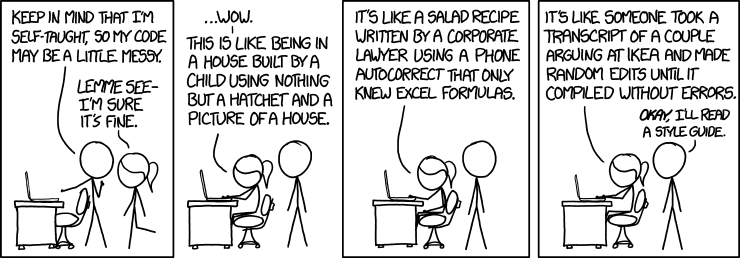
\includegraphics[width=\linewidth]{./gfx/xkcd-codeQuality}
\caption
	[Code Quality]
	{Code Quality. Quelle: \url{https://xkcd.com/1513/}}
\end{center}
\end{figure}
Immer wieder wird die Frage gestellt, welche Programmteile sinnvoll in Funktionen ausgelagert werden sollten und welche nicht. Während es dafür keine allgemeingültige Formel gibt, kann man zumindest einige Situationen aufführen, in denen es sich anbietet, Code in einer eigenen Funktion anzulegen.

Generell ist es sinnvoll, alle Arbeitsschritte, die eine gedankliche Einheit bilden, in einer Funktion zu verkapseln. Eine gedankliche Einheit ist etwa \enquote{Berechne den Wert einer Funktion} oder \enquote{Gib Text auf dem Bildschirm aus}.

Insbesondere sollte aller Code, den man mehrfach verwenden will in Funktionen stehen. Kopierter Code macht das Programm länger und damit schwieriger zu warten. Vor allem aber ergibt sich daraus eine Fehlerquelle, da Änderungen an einem kopierten Codeteil verlangen, auch alle anderen Stellen zu ändern, an denen diese Kopien auftauchen. Es ist leicht, diese Stellen zu vergessen und so inkonsistenten und fehlerhaften Code zu erhalten.

Schließlich kann es von Vorteil sein, selbst Codeblöcke in Funktionen zu setzen, die nur einmal aufgerufen werden. Ein Funktionsname sollte eindeutig beschreiben, welche Aufgabe die Funktion erfüllt. Ist dies gegeben, so kann der Ablauf eines Programms klarer im Code gelesen werden, ohne jedes Detail Zeile für Zeile nachvollziehen zu müssen. Sehen Sie sich dazu folgenden Code an:

\begin{codebox}[Beispiel: \texttt{main} eines Spiels]
\begin{minted}[linenos]{c}
/* ... #include-Zeilen stehen hier ... */

/* ... Funktionen stehen hier ... */

int main () {
  showTitleAnimation();

  int selectedMenuPoint = 0;
  do {
    showMenuScreen();
    selectedMenuPoint = askForMenuOption();
    performAction(selectedMenuPoint);
  } while(selectedMenuPoint);
}
\end{minted}
\end{codebox}

Hier wird vor Start des Spiels eine Animation gezeigt. Im Anschluss wird jeweils in Folge ein Menü\-bildschirm dargestellt, eine Usereingabe angenommen und dann dafür gesorgt, dass die Auswahl des Users ausgeführt wird. Dies wird solange durchgeführt, bis die Funktion \texttt{askForMenuOption} den Wert~\texttt{0} zurückgibt. Dies könnte (und sollte) \eg dann der Fall sein, wenn der User auswählt, das Spiel zu beenden.

Obwohl in diesem Beispiel nicht klar ist, wie die Animation im Detail aussieht, oder welche Menüpunkte angeboten werden, ist klar, wie das Programm organisiert ist. Neue Features können leicht eingefügt werden. Soll etwa eine Animation ausgeführt werden, sobald ein Menupunkt ausgewählt wurde, so kann nach Zeile 11 noch eine neue Funktion \texttt{showMenuAnimation(selectedMenuPoint)} eingefügt werden.

Funktionen können sich auch untereinander aufrufen, wie wir in Abschnitt \ref{sec:forwardDeclaration} gesehen haben. Dies \enquote{kostet} einigen Verwaltungsaufwand (um den wir als ProgrammiererInnen uns aber nicht explizit kümmern müssen). Der Compiler muss für jeden Aufruf einer Funktion mitspeichern, an welche Stelle bei Verlassen der aufgerufenen Funktion zurück gesprungen werden soll; außerdem müssen die Speicherbereiche für die einzelnen Funktionen angelegt und wieder frei gegeben werden. Bei geringer \emph{Aufruftiefe} (bis etwa 20 Aufruf-Ebenen) fällt dies nicht weiter ins Gewicht. Stärkere Verschachtelung macht Programme aber merklich langsamer. Natürlich ist es vor allem schwierig, eine Struktur mit so vielen Ebenen zu überblicken. Daher möchte ich Ihnen diesen Gedanken als einzige Beschränkung für die Sinnhaftigkeit von Funktionen mitgeben: halten Sie die Verschachtelung klein und übersichtlich. In Kapitel \ref{chp:recursion} werden wir diesen Gedanken nochmals aufgreifen.

\subsection{Rückgabe mehrerer Werte}
Eine Funktion kann nur entweder nichts (\mintinline{c}{void}) oder genau einen einzigen Wert zurückgeben. Es gibt aber Situationen, in denen dieselbe Funktion \emph{mehrere} Werte zugleich berechnen soll. Um dies zu ermöglichen stehen uns zwei Techniken zur Verfügung: Wir können ein \emph{Array} oder ein \mintinline{c}{struct} zurückgeben.

Arrays werden über Pointer verwaltet, daher muss der Rückgabetyp auch ein Pointer sein. (Tatsächlich gibt unsere Funktion also nur einen einzigen Wert zurück; dieser gibt dann aber eine Speicherstelle an, an der alle berechneten Werte zu finden sind.)

Sehen Sie sich folgendes Beispiel an, das ein Rezept für Obstsalat auf verschiedene Menschenmengen anpasst:

\begin{codebox}[Beispiel: Umrechnung eines Rezepts]
\begin{minted}[linenos]{c}
#include <stdio.h>
#include <stdlib.h>
// https://www.chefkoch.de/rezepte/654221166964999/Bunter-Obstsalat.html

double * fruitsaladForPersons(double persons) {
  double * reVal = malloc(8 * sizeof(*reVal));

  reVal[0] = persons/4.0 *   3;  // apples
  reVal[1] = persons/4.0 *   2;  // bananas
  reVal[2] = persons/4.0 *   2;  // peaches
  reVal[3] = persons/4.0 *   2;  // kiwis
  reVal[4] = persons/4.0 *   1;  // mangos
  reVal[5] = persons/4.0 *   1;  // oranges
  reVal[6] = persons/4.0 * 200;  // grams of grapes
  reVal[7] = persons/4.0 *  50;  // grams of walnuts

  return reVal;
}

int main () {
  double persons = 2;
  double * requirements = fruitsaladForPersons(persons);

  printf("Obstsalat für %1.0lf Personen:\n", persons);
  printf("\tÄpfel    : %5.1lf\n"  , requirements[0]);
  printf("\tBananen  : %5.1lf\n"  , requirements[1]);
  printf("\tPfirsiche: %5.1lf\n"  , requirements[2]);
  printf("\tKiwis    : %5.1lf\n"  , requirements[3]);
  printf("\tMangos   : %5.1lf\n"  , requirements[4]);
  printf("\tOrangen  : %5.1lf\n"  , requirements[5]);
  printf("\tTrauben  : %5.1lf g\n", requirements[6]);
  printf("\tWalnüsse : %5.1lf g\n", requirements[7]);

  free(requirements);
}
\end{minted}
\end{codebox}

\begin{cmdbox}[Ausführungsbeispiel: Umrechnung eines Rezepts]
\begin{minted}{text}
Obstsalat für 2 Personen:
        Äpfel    :   1.5
        Bananen  :   1.0
        Pfirsiche:   1.0
        Kiwis    :   1.0
        Mangos   :   0.5
        Orangen  :   0.5
        Trauben  : 100.0 g
        Walnüsse :  25.0 g
\end{minted}
\end{cmdbox}

Beachten Sie hier auch, dass der in Zeile 5 reservierte Speicherbereich wieder freigegeben werden muss. Dies geschieht in Zeile 35.

\mintinline{c}{struct}s werden in Kapitel \ref{chp:structs} besprochen.

\subsection{Speicherklasse \mintinline{c}{static}} \label{sec:staticVar}
Variablen sind immer nur in ihrem aktuellen Scope sichtbar, und werden \idR zerstört, sobald der aktuelle Scope verlassen wird. Manchmal soll aber der Wert einer Speicherstelle erhalten bleiben, selbst wenn die Ausführung den Scope verlässt, in dem die Variable definiert wurde. Bisher können wir dies nur lösen, indem wir die entsprechende Variable in einem Scope anlegen, das für die gesamte Lebensdauer des Programms existiert (also in der \texttt{main} oder als globale Variable), und einen Pointer auf diesen Wert \enquote{durchreichen}.

\begin{codebox}[Beispiel: Funktionsaufrufe mitzählen (1)]
\begin{minted}[linenos]{c}
#include <stdio.h>

void foobar(int * callCounter) {
  (*callCounter)++;
  printf("Aufruf #%d\n", *callCounter);
}

int main () {
  int calls = 0;

  foobar(&calls);
  foobar(&calls);
}
\end{minted}
\end{codebox}

\begin{cmdbox}[Ausführungsbeispiel: Funktionsaufrufe mitzählen (1)]
\begin{minted}{text}
Aufruf #1
Aufruf #2
\end{minted}
\end{cmdbox}

Dieser Code funktioniert zwar, ist aber fehleranfällig. Zunächst muss ein Anwender den Zweck von \texttt{calls} kennen, um die Funktion \texttt{foobar} richtig zu nutzen. Insbesondere darf \texttt{calls} nicht versehentlich geändert werden. Nicht zuletzt \enquote{belegt} diese Technik einen Variablennamen in der \texttt{main}.

Als Alternative dazu können Variablen in der Funkton \texttt{foobar} mit dem Schlüsselwort \mintinline{c}{static} deklariert werden. Auf diese Weise bleibt die Speicherstelle reserviert, \ie gespeicherte Werte erhalten, auch wenn die Funktion später wieder aufgerufen wird. Der Scope-Mechanismus hingegen wird nicht außer Kraft gesetzt. In Code sieht das dann so aus:

\begin{codebox}[Beispiel: Funktionsaufrufe mitzählen (2)]
\begin{minted}[linenos]{c}
#include <stdio.h>

void foobar() {
  static int callCounter = 0;
  callCounter++;
  printf("Aufruf #%d\n", callCounter);
}

int main () {
  foobar();
  foobar();
  // printf("%d\n", callCounter); -- unzulässig, falscher Scope
}
\end{minted}
\end{codebox}

Der Compiler legt \emph{ein einziges Mal} die Speicherstelle für \texttt{callCounter} an, selbst wenn (wie hier) die Funktion \texttt{foobar} mehrfach aufgerufen wird. Entsprechend findet auch die Wertzuweisung in Zeile 4 nur ein einziges Mal statt. Danach \enquote{erinnert} sich der Compiler an die bereits angelegte Speicherstelle sobald \texttt{foobar} \enquote{betreten} wird, \enquote{vergisst} aber diesen Variablennamen (nicht aber die Speicherstelle selbst) wieder, wenn die Funktion verlassen wird.

\section{Optimierung: \mintinline{c}{inline}} \label{sec:inline}
Bei einem Funktionsaufruf werden die Werte von Parametern kopiert.  Ebenso wird die Stelle gespeichert, von der weg gesprungen wurde, so dass beim Verlassen der Funktion die Ausführung nach dem Sprung-Befehl dort fortgesetzt werden kann. Dieses Kopieren und Speichern kostet Zeit. Bei häufig wiederkehrenden Aufrufen führt dies zu merklichen Performance-Einbrüchen.

Um dem entgegen zu wirken, können \emph{kurze} Funktionen als \mintinline{c}{inline} deklariert werden\footnote{Es gibt allerdings keine Garantie dafür, dass der Compiler die Funktion wirklich an entsprechende Stellen im einfügt. Es handelt sich also lediglich um einen Hinweis an den Compiler.}. Dies teilt dem Compiler mit, dass der Funktionskörper an der aufrufenden Stelle eingefügt werden sollte, statt einen normalen Sprung und Rücksprung durchzuführen. Ergebnis ist eine größere ausführbare Datei (da derselbe Code an mehreren Stellen eingefügt wird), der aber schneller läuft. Für die ProgrammiererInnen ergibt sich sonst kein Unterschied -- Funktionsaufruf sowie Scoping funktionieren wie bisher besprochen.

Um eine Funktion als \mintinline{c}{inline} zu deklarieren, schreibt man eine forward declaration und stellt dieser das Schlüsselwort \mintinline{c}{inline} voran:

\begin{codebox}[Syntax: \texttt{inline}-Funktion]
\begin{minted}{c}
inline Rückgabetyp Funktionsname (Parameterliste);
\end{minted}
\end{codebox}

\begin{codebox}[Beispiel: Maximum von zwei Ganzzahlen finden]
\begin{minted}[linenos]{c}
inline int max (int a, int b);
       int max (int a, int b) {return a > b   ?   a  :  b;}
\end{minted}
\end{codebox}

\section{Funktionszeiger} \label{sec:funcPtr}
Alle Objekte mit denen wir arbeiten müssen im Speicher abgelegt werden. Sie haben daher notwendigerweise auch eine Adresse. Dies umfasst einzelne Zahlen, Gruppen von Zahlen (Arrays) und eben auch Programmcode. Bei der Ausführung eines Programms wird dieses zunächst in den Arbeitsspeicher kopiert, und dann die Maschinencode-Anweisungen ausgeführt, die in der Datei vermerkt waren. Wir können die Adressen von bestimmten Programmteilen ausfindig machen und mit der Ausführung an diese Adressen springen. Zu diesem Zweck existiert das Konzept von \texttt{Funktionszeigern}, also Pointer auf Funktionen.

Funktionszeiger sind wie alle Pointer Variablen, die zunächst deklariert werden müssen. Diese Deklaration enthält alle Informationen der Funktionssignatur, also Rückgabewert der Funktion und Parameterliste. Dies drückt sich in der folgenden (leider etwas unhandlichen Syntax) aus:
\begin{codebox}[Syntax: Deklaration Funktionszeiger]
\begin{minted}{c}
Rückgabetyp (*Variablenname) (Parameterliste);
\end{minted}
\end{codebox}

Solchen Variablen kann nun die Adresse einer beliebigen Funktion (mit passender Signatur) zugewiesen werden. Dies geschieht \emph{ohne} jegliche Operatoren, einfach über den Funktionsnamen:

\begin{codebox}[Beispiel: Funktionszeiger (1)]
\begin{minted}[linenos]{c}
#include <stdio.h>

void foo() {
  printf("blerb.\n");
}

int main () {
  void (*funcPtr)() = foo;
}
\end{minted}
\end{codebox}

Der Codeabschnitt, auf den dieser Funktionspointer zeigt, kann nun mit dem neuen Symbol \texttt{funcPtr} aufgerufen werden, ganz als würde man direkt mit \texttt{foo} arbeiten:

\begin{codebox}[Beispiel: Funktionszeiger (2)]
\begin{minted}[linenos]{c}
#include <stdio.h>

void foo() {
  printf("blerb.\n");
}

int main () {
  void (*funcPtr)() = foo;
\end{minted}
\end{codebox}
%
\begin{codebox}[]
\begin{minted}[linenos]{c}
  printf("direkt : ");
  foo();

  printf("funcPtr: ");
  funcPtr();
}
\end{minted}
\end{codebox}

\begin{cmdbox}[Ausführungsbeispiel: Funktionszeiger (2)]
\begin{minted}{text}
direkt : blerb.
funcPtr: blerb.
\end{minted}
\end{cmdbox}

\begin{hintbox}
Der Name einer Funktion beschreibt selbst einen Funktionszeiger! Der Aufruf einer Funktion ist eine \emph{Operation}, vergleichbar mit dem Dereferenzieren (Operator \texttt{*}). Daher müssen auch Funktionen, die keine Parameter erwarten, mit leeren Klammern () aufgerufen werden.
\end{hintbox}

Der Zweck dieser Technik ist, das Verhalten anderer Funktionen vom Ergebnis anderer Berechnungen abhängig zu machen, ohne sich dabei auf die Art der Berechnung festzulegen.

Als Beispiel sei die Funktion \texttt{qsort}\footnote{Der Sortieralgorithmus \emph{quicksort}, der dieser Funktion zugrunde liegt, wird in der Vorlesung \emph{Algorithmen und Datenstrukturen} an der Universität Regensburg genauer besprochen.} genannt (definiert in \texttt{stdlib.h}). Diese Funktion kann Arrays beliebigen Typs nach beliebigen Kriterien sortieren. Die Sortier-Kriterien werden in Form einer Funktion \texttt{comp} beschrieben, die zwei Werte \texttt{a} und \texttt{b} miteinander vergleicht. (Hier verwende ich den Namen \texttt{comp}, um den folgenden Abschnitt leichter lesbar zu halten; die Vergleichsfunktion darf in der Anwendung aber einen beliebigen Namen haben.)

Da Arrays \emph{beliebigen} Typs sortiert werden, können an \texttt{comp} nicht die \emph{Werte} \texttt{a} und \texttt{b} übergeben werden, sondern nur ihre \emph{Adressen} \texttt{\&a} und \texttt{\&b}.

Wenn \texttt{a} \emph{vor} \texttt{b} in der sortierten Liste auftauchen soll, soll der Rückgabewert von \texttt{comp(\&a, \&b)} gleich \texttt{-1} sein. Falls dagegen \texttt{b} vor \texttt{a} sortiert werden soll, so muss \texttt{+1} zurückgegeben werden. Schließlich wird \texttt{comp} den Wert \texttt{0} zurückgeben, wenn \texttt{a} und \texttt{b} gleichwertig sind. (\emph{Gleichwertig} bedeutet in diesem Kontext nicht zwingend \emph{gleich}. Wir könnten zum Beispiel Zahlen nach ihrer Quersumme sortieren. Für diese Sortierung sind die Zahlen \texttt{19} und \texttt{91} dann gleichwertig, nicht aber gleich.)

Die \href{https://en.cppreference.com/w/c/algorithm/qsort}{cpp-Referenz} teilt uns die Signatur der Funktion \texttt{qsort} mit:

\begin{codebox}[Prototyp der Funktion \texttt{qsort}]
\begin{minted}{c}
void qsort( void * ptr, size_t count, size_t size,
            int (*comp)(const void *, const void *) );
\end{minted}
\end{codebox}

Betrachten wir die einzelnen Parameter:
\begin{itemize}
\item Der erste Parameter \texttt{ptr} ist ein Pointer auf ein beliebiges Array und daher vom Typ
		\mintinline{c}{void *}.
\item Mit \texttt{count} wird die Zahl der Elemente des Arrays beschrieben. (Der Typ
		\mintinline{c}{size_t} ist ein Alias (ein alternativer Name) für \mintinline{c}{unsigned int}.)
\item Der Wert \texttt{size} beschreibt den Speicherbedarf \emph{eines} Elements des Arrays. Wir
		brauchen diese Information, da \texttt{qsort} \ua für \mintinline{c}{int}-,
		\mintinline{c}{double}- oder \mintinline{c}{char}-Arrays funktionieren soll, die allesamt
		unterschiedlichen Speicherbedarf haben.
\item Die letzte Zeile schließlich benennt den Parameter \texttt{comp}, der eine Vergleichsfunktion
		benennt. Diese Funktion wird einen \mintinline{c}{int} zurück geben, und nimmt zwei
		\mintinline{c}{const void *} als Argumente an. Dabei bedeutet \mintinline{c}{const} wieder, dass
		\texttt{comp} die Werte von \texttt{a} und \texttt{b} nur lesen, nicht aber verändern wird.
		Der Modifier \mintinline{c}{const} gehört zum Datentyp und muss daher auch in unserer Funktions-
		Signatur auftauchen. Wieder gilt: Da der Datentyp von \texttt{a} und \texttt{b} beliebig ist,
		können nur \mintinline{c}{void *} übergeben werden.
\end{itemize}

Mit diesen Informationen können wir das (leicht abgewandelte) Beispiel von der \href{https://en.cppreference.com/w/c/algorithm/qsort}{cpp-Referenz} verstehen:

\begin{codebox}[Beispiel: \texttt{qsort} mit zwei Sortiermethoden]
\begin{minted}[linenos]{c}
#include <stdio.h>
#include <stdlib.h>

int comp_ascending(const void* a, const void* b) {
    int arg1 = *(const int *) a;
    int arg2 = *(const int *) b;

    if (arg1 < arg2) return -1;
    if (arg1 > arg2) return  1;
    return 0;
}

int comp_descending(const void* a, const void* b) {
    return -comp_ascending(a, b);
}

int main(void) {
    int ints[] = { -2, 99, 0, -743, 2, 4 };
    int size = sizeof(ints) / sizeof(*ints);

    printf("Aufsteigende Sortierung:\n");
    qsort(ints, size, sizeof(int), comp_ascending);

    for (int i = 0; i < size; i++) {
        printf("%d ", ints[i]);
    }
    printf("\n");

    printf("Absteigende Sortierung:\n");
    qsort(ints, size, sizeof(int), comp_descending);

    for (int i = 0; i < size; i++) {
        printf("%d ", ints[i]);
    }
    printf("\n");
}
\end{minted}
\end{codebox}

\begin{cmdbox}[Ausführungsbeispiel: \texttt{qsort} mit zwei Sortiermethoden]
\begin{minted}{text}
Aufsteigende Sortierung:
-743 -2 0 2 4 99
Absteigende Sortierung:
99 4 2 0 -2 -743
\end{minted}
\end{cmdbox}

Obwohl die Funktion \texttt{qsort} nur einmal programmiert wurde, kann sie mit diesen Techniken also \emph{generisch} benutzt werden, \ie sie ist für viele verschiedene Zwecke einsetzbar, die bei der Erstellung von \texttt{qsort} noch nicht einmal vorgesehen waren.

%	\include{10_Structs}
%	\chapter{Modulare Programmierung}\label{chp:modules}
\epigraph{Everything is awesome!}{Emmet Brickowski}

Für besonders große Projekte bietet es sich an, den Code auf mehrere Dateien zu verteilen, und diese nach Aufgaben zu sortieren. Dies erlaubt es, eine \enquote{übergeordnete} Kapselung umzusetzen, die ähnlich funktioniert wie schon bei den Funktionen besprochen wurde (siehe Kapitel \ref{chp:funcs}), und die den Einfluss begrenzt, den die einzelnen Programmkomponenten aufeinander haben.

Ein \emph{Modul} ist eine C-Code-Datei, die nur \enquote{ihre eigenen} Variablen und Funktionen \enquote{sieht}. Innerhalb eines Moduls müssen alle Namen (von Variablen, Funktionen, Sprung-Labels, ...) eindeutig sein, \ie dürfen nicht doppelt vergeben werden (es sei denn, sie \enquote{leben} jeweils in ihrem eigenen Scope). Ein Modul erzeugt allerdings wiederum einen umfassenden Scope; daher dürfen in zwei getrennten Modulen dieselben Namen vorkommen.

Verbunden werden Module über \emph{Header}-Dateien, die lediglich Definitionen enthalten. Diese Definitionen teilen gewissermaßen mit, welche Funktionen, Variablen, ... geteilt werden, also über die Modulgrenzen hinaus sichtbar sein sollen.

\section{Trennung von Header- und Modul-Code}
Wir haben Header schon im Kontext von Libraries kennen gelernt: mittels \mintinline{c}{#include}-Zeilen laden wir die nötigen Definitionen, die wir benötigen, um die Funktionen der Libraries zu benutzen. Dem Compiler haben wir mit Kommandozeilenoptionen wie \texttt{-lm} mitgeteilt, dass die im Header definierten Funktionen in einem vorkompilierten Modul zu finden sind. Stellen Sie sich im Folgenden vor, der Befehl \mintinline{c}{#include} würde per Copy\&Paste den Inhalt der includierten Datei in Ihren Code einfügen.

Die Organisation eines Projekts in Module geschieht mit derselben Mechanik; jedoch bieten wir hier zum \emph{Linken} keine vorkompilierte Bibliothek, sondern tatsächlichen C-Code. Der Header definiert also eine Schnittstelle zwischen den einzelnen Komponenten.

Eine Header-Datei endet auf die Erweiterung \texttt{.h} und darf prinzipiell beliebigen C-Code enthalten. Sinnvoll ist es jedoch, hier nur \emph{Definitionen} zu setzen, also Anweisungen, die keinen Einfluss auf die Speicherstruktur haben. Definitionen sind \eg Funktions-Signaturen (siehe Abschnitt \ref{sec:forwardDeclaration}), \mintinline{c}{struct}s und \mintinline{c}{typedef}s (siehe Kapitel \ref{chp:structs}). Deklarationen von \emph{Variablen} dagegen dürfen im Header nicht vorkommen, da die Deklaration auch eine Speicherstelle reserviert, \ie die Speicherstruktur verändert.

Bislang haben wir nur \mintinline{c}{#include}-Zeilen gesehen, bei denen der Header-Name von <spitzen Klammern> eingefasst war. Dies teilt dem Compiler mit, dass die Header-Datei in einem Standard-Verzeichnis zu finden ist, das bei der Installation des Compilers angelegt wird. Da sich unsere Header \idR im selben Verzeichnis befinden wie unser Code, fassen wir diese stattdessen mit \texttt{"}doppelten Anführungszeichen\texttt{"} ein.

Als Beispiel wollen wir uns vorstellen, wir wollen eine eigene library anlegen, die den Umgang mit 2D-Punkten erleichtert. Wir definieren zuerst im Header \texttt{vector2D.h} einen Datentypen und \enquote{machen die Funktionen des Moduls sichtbar}:

\begin{codebox}[Beispiel: Header \texttt{vector2D.h}]
\begin{minted}[linenos]{c}
typedef struct {
  double x;
  double y;
} vector2D;

vector2D v2_sum     (vector2D a, vector2D b);
vector2D v2_inv     (vector2D v);
vector2D v2_scale   (vector2D v, double f);
double   v2_dotProd (vector2D a, vector2D b);
double   v2_length  (vector2D v);
\end{minted}
\end{codebox}

Die \emph{Implementierung} hierzu speichern wir in der Datei \texttt{vector2D.c}:

\begin{codebox}[Beispiel: Modulcode \texttt{vector2D.c}]
\begin{minted}[linenos]{c}
#include "vector2D.h"
#include <math.h>

vector2D v2_sum     (vector2D a, vector2D b) {
  vector2D reVal = {a.x + b.x, a.y + b.y};
  return reVal;
}

vector2D v2_inv     (vector2D v)             {
  vector2D reVal = {-v.x, -v.y};
  return reVal;
}

vector2D v2_scale   (vector2D v, double f)   {
  vector2D reVal = {f * v.x, f * v.y};
  return reVal;
}

double   v2_dotProd (vector2D a, vector2D b) {return a.x * b.x + a.y * b.y;}
double   v2_length  (vector2D v)             {return hypot(v.x, v.y);}
\end{minted}
\end{codebox}

Da in diesem Modul mit der Definition des Typs \texttt{vector2D} gearbeitet wird, muss diese Definition auch \enquote{sichtbar} sein. Daher laden wir in den Modulcode den Header mittels \mintinline{c}{#include} (Zeile 1). Weiter benutzen wir die Funktion \texttt{hypot} (berechnet den Wert $\sqrt{x^{2} + y^{2}}$, also die Länge eines Vektors $\begin{pmatrix}
x \\ y
\end{pmatrix}$). Diese Funktion ist im Header \texttt{<math.h>} definiert, weswegen dieser ebenfalls geladen wird. Während \texttt{vector2D.h} in unserem Arbeitsverzeichnis liegt und daher mit \texttt{"}doppelten Anführungszeichen\texttt{"} eingefasst wird, findet sich \texttt{math.h} in einem Standard-Verzeichnis, und ist deswegen durch \texttt{<}spitze Klammern\texttt{>} eingefasst.

Achtung: Die Datei \texttt{vector2D.c} besitzt \emph{keine} Funktion \texttt{main}! Sie kann vom Compiler zu \emph{Object-Code} umgesetzt werden, \ie in Maschinensprache übersetzt werden; Linken zu einem \emph{ausführbaren Programm} ist mit diesem Code alleine jedoch nicht möglich.

Das \emph{Hauptmodul} findet sich in einer eigenen Datei \texttt{myProgram.c}:

\begin{codebox}[Beispiel: Hauptmodulcode \texttt{myProgram.c}]
\begin{minted}[linenos]{c}
#include <stdio.h>
#include "vector2D.h"

int main () {
  vector2D v = {1,1}, w = {2, 3};

  printf("%lf\n", v2_length(v2_sum(v, w)));
}
\end{minted}
\end{codebox}

Hier stehen nun alle \enquote{Befehle} zur Verfügung, die wir im Header \texttt{vector2D.h} deklariert haben. Wir müssen hier nicht explizit die Bibliothek \texttt{<math.h>} einbinden, da keine Funktion aus der math-library im Hauptmodul explizit benutzt wird.

Unser Projekt besteht also aus zwei Modulen, die über einen gemeinsamen Header verbunden sind. Diese beiden Module müssen beim Aufruf des Compilers aufgeführt werden:

\begin{cmdbox}[Compileraufruf: Projekt aus zwei Modulen]
gcc -std=c11 -Wall -Wextra -Wpedantic myProgram.c vector2D.c -lm -o myProgram
\end{cmdbox}

Achtung: der hier gezeigte Aufruf besteht nur aus einer \emph{einzigen Zeile}. Wenn Sie diesen Aufruf eintippen bedarf es \emph{keines} Zeilenumbruchs nach \texttt{-lm}. Beachten Sie weiter auch, dass im Compiler-Aufruf der Header \emph{nicht} erwähnt wird!

Wie üblich findet das Kompilieren über den \texttt{gcc} statt. Wir listen zunächst einige Optionen auf (C-Standard von 2011, Anzeigen aller relevanten Warnungen) und nennen dann unsere beiden Module (\texttt{myProgram.c} und \texttt{vector2D.c}). Den Zusatz \texttt{-lm} kennen wir als Compiler Option um die Math-Library einzubinden. Wir können dies als ein \emph{drittes} Modul auffassen, das in unserem Projekt verwendet wird. Schließlich nennen wir mit \texttt{-o myProgram} den Namen der ausführbaren Datei, die aus unserem Code erzeugt werden soll.


\section{Speicherklasse \mintinline{c}{extern}}
Wo globale Variablen über Modulgrenzen hinaus zur Verfügung stehen sollen, kommt das Schlüsselwort \mintinline{c}{extern} zum Einsatz. Es wird einer Variablen-Deklaration vorangestellt, und teilt dem Compiler mit dass an einer anderen Stelle eine Variable mit diesem Namen deklariert wird, und dass diese Variable im aktuellen Modul sichtbar sein soll. Mit einer \mintinline{c}{extern}-Deklaration wird also \emph{keine Speicherstelle} reserviert!

Betrachten Sie folgende drei Dateien:

\begin{codebox}[Beispiel: Hauptmodulcode \texttt{myProg.c}]
\begin{minted}[linenos]{c}
#include <stdio.h>
#include "definitions.h"

int main () {
  printf("Globale Variable 'global' = %lf\n", global);
}
\end{minted}
\end{codebox}

\begin{codebox}[Beispiel: Header \texttt{definitions.h}]
\begin{minted}[linenos]{c}
extern double global;
\end{minted}
\end{codebox}

\begin{codebox}[Beispiel: Modul \texttt{module.c}]
\begin{minted}[linenos]{c}
#include "definitions.h"

double global = 5.0;
\end{minted}
\end{codebox}

Im Hauptmodul \texttt{myProg.c} wird in Zeile 5 Bezug auf eine Variable \texttt{global} genommen. Dass eine solche Variable existiert wird über den Header \texttt{definitions.h} mitgeteilt. Die dortige Zeile \mintinline{c}{extern double global;} legt aber noch nicht die Variable an, sondern teilt dem Compiler nur mit, dass es ein Objekt mit dem Namen \texttt{global} gibt. Dieses Objekt wird schließlich im Modul \texttt{module.c} angelegt und erhält dort in Zeile 3 den Wert \texttt{5.0}.

\begin{warnbox}[\texttt{extern}-Anweisungen sind reine Definitionen]
\mintinline{c}{extern}-Zeilen legen keine Speicherstellen an; sie reservieren lediglich ein Symbol. Zu jedem \mintinline{c}{extern} muss es ein Gegenstück geben, das tatsächlichen Speicher belegt. Dieses Gegenstück muss \emph{eindeutig} sein, \ie es darf nur eine einzige \enquote{echte} Variable geben, die den Namen trägt, der in der \mintinline{c}{extern}-Zeile referenziert wird.

Da \mintinline{c}{extern} nur ein Symbol benennt, schreiben wir diesen Befehl in die Header-Dateien. Die zugehörige Speicherstelle \enquote{lebt} in (genau) einem Modul.
\end{warnbox}

Wozu dieser Aufwand? Sollte es nicht genügen, eine Variable direkt in einem Header zu deklarieren?

Betrachten Sie dazu folgendes Codebeispiel:
\begin{codebox}[Beispiel: Hauptmodulcode \texttt{myProg.c}]
\begin{minted}[linenos]{c}
#include <stdio.h>
#include "definitions.h"

int main () {
  printf("Globale Variable 'global' = %lf\n", global);
}
\end{minted}
\end{codebox}

\begin{codebox}[Beispiel: Header \texttt{definitions.h}]
\begin{minted}[linenos]{c}
double global = 5;

void setGlobalToSeven();
\end{minted}
\end{codebox}

\begin{codebox}[Beispiel: Modul \texttt{module.c}]
\begin{minted}[linenos]{c}
#include "definitions.h"

void setGlobalToSeven() {
  global = 7;
}
\end{minted}
\end{codebox}

Dieses Dateipaket lässt sich nicht kompilieren. Der Linker (\ie der \texttt{gcc}) gibt folgende  Fehlermeldung aus:

\begin{cmdbox}[Fehlermeldung des Linkers]
/tmp/cccuG8Y5.o:(.data+0x0): Mehrfachdefinition von »global«
/tmp/cc3AiH0L.o:(.data+0x0): hier zuerst definiert
collect2: error: ld returned 1 exit status
\end{cmdbox}

Wieso ist das so?

Der Header \texttt{definitions.h} wird von beiden Modulen (\texttt{myProg.c} und \texttt{module.c}) benötigt, da die Variable \texttt{global} in beiden zur Verfügung stehen soll. Daher enthalten beide Module auch die Zeile \mintinline{c}{#include "definition.h"}. Der Header-Code wird also in beiden Dateien \enquote{eingefügt}. Diese Header-Code enthält aber auch die \emph{Deklaration} von \texttt{global}. Effektiv wird die Variable also zweimal deklariert! Der Compiler kann nicht entscheiden, welche der beiden Deklarationen \enquote{die Richtige} ist; daher bricht der Linking-Vorgang ab.

\begin{warnbox}[Keine Deklarationen in Headern]
Wie bereits erwähnt sollen in Headern nur Definitionen stehen, \ie \mintinline{c}{struct}s, \mintinline{c}{union}s, \mintinline{c}{enum}s \mintinline{c}{typedef}s, \mintinline{c}{extern}s und Funktions-Prototypen. Bei all diesen Anweisungen werden noch keine Speicher-Stellen reserviert, sondern lediglich \enquote{Formen} definiert.

Da Header den Zweck haben, mehrere Module miteinander zu verbinden, werden sie in mindestens zwei Dateien inkludiert. Eine Deklaration in einem Header wird also naturgemäß zu doppelten Deklarationen führen. Aus diesem Grund schreiben wir in einen Header \emph{ausschließlich} Definitionen. Alle Anweisungen, die die Struktur des Speichers verändern, \enquote{leben} in Modulen.
\end{warnbox}

\section{Funktionen mit eingeschränkter Sichtbarkeit: \mintinline{c}{static}}
Wir kennen das Schlüsselwort \mintinline{c}{static} bereits aus dem Kontext von Funktionen: Variablen, die mit diesem Modifier deklariert werden, verbleiben im Speicher, selbst wenn ihr Symbol durch verlassen des Scopes nicht mehr gültig ist. (Siehe Abschnitt \ref{sec:staticVar}.)

Im Kontext Module hat das Schlüsselwort \mintinline{c}{static} jedoch noch eine zweite Bedeutung:

Selbst, wenn Funktionen nur innerhalb eines Moduls gebraucht werden und nicht im Header \enquote{sichtbar gemacht werden}, müssen ihre Namen über das gesamte Projekt hinweg eindeutig sein, dürfen also nicht doppelt vorkommen. Soll diese Regel aufgehoben werden, kann eine Funktion mit dem Schlüsselwort \mintinline{c}{static} als außerhalb der Modulgrenzen \enquote{unsichtbar} markiert werden.

Betrachten Sie hierzu folgende Dateistruktur\footnote{Wie tatsächlich Zufallszahlen generiert werden können, wird im Abschnitt \ref{sec:RandomNums} besprochen.}:

\begin{codebox}[Beispiel: Hauptmodulcode \texttt{myProg.c}]
\begin{minted}[linenos]{c}
#include <stdio.h>
#include "definitions.h"
\end{minted}
\end{codebox}
%
\begin{codebox}[]
\begin{minted}[linenos, firstnumber=last]{c}
// https://xkcd.com/221/
static int getRandomNumber () {
  return 4;   // chosen by a fair dice roll.
              // guaranteed to be random.
}

int main () {
  printf("Random Number %d\n", getRandomNumber());
  printf("Random Event: %s\n", getRandomEvent ());
}
\end{minted}
\end{codebox}

\begin{codebox}[Beispiel: Header \texttt{definitions.h}]
\begin{minted}[linenos]{c}
char * getRandomEvent ();
\end{minted}
\end{codebox}

\begin{codebox}[Beispiel: Modul \texttt{module.c}]
\begin{minted}[linenos]{c}
#include <stdlib.h>

static int getRandomNumber() {return rand() % 3;}

char * getRandomEvent () {
  switch (getRandomNumber()) {
    case 0 :
      return "Zeppelin!";      // https://xkcd.com/73/
    case 1 :
      return "Wild Ratata!";
    case 2 :
      return "Tree-Powers, activate!";
  }
  return "The inexonerable passage of time";
}
\end{minted}
\end{codebox}

Hier haben sowohl \texttt{myProg.c} als auch \texttt{module.c} eine Funktion mit Namen \texttt{getRandomNumber}. Da aber beide als \mintinline{c}{static} ausgezeichnet sind, \enquote{kommen sie sich nicht in die Queere}. Wird bei nur einer der beiden das Schlüsselwort \mintinline{c}{static} entfernt, ergeben sich ebenfalls noch keine Probleme: Die Situation hier ist grob vergleichbar mit zwei sich umschließenden Scopes. Wenn aber beide Instanzen von \texttt{getRandomNumber} ohne die Auszeichnung \mintinline{c}{static} im Code auftauchen, meldet der Linker eine doppelte Definition:

\begin{cmdbox}[Fehlermeldung des Linkers: Mehrfachdefinition von \texttt{getRandomNumber}]
\begin{minted}{text}
/tmp/ccXCopXE.o: In Funktion »getRandomNumber«:
module.c:(.text+0x0): Mehrfachdefinition von »getRandomNumber«
/tmp/cc3SiANo.o:myProgram.c:(.text+0x0): hier zuerst definiert
collect2: error: ld returned 1 exit status
\end{minted}
\end{cmdbox}

\section{Weitere Speicherklassen und Modifier}
Die folgenden Typen-Modifier sind hier nur der Vollständigkeit halber aufgeführt und können z.\,T. nur mit vertieften Kenntnissen über Prozessorarchitektur wirklich verstanden werden.
\begin{description}
\item[auto] Die Speicherklasse \mintinline{c}{auto} ist die Standard-Speicherklasse und wird überall
	dort verwendet, wo nicht explizit \mintinline{c}{static} oder \mintinline{c}{extern} gesetzt wird.
\item[register] wird für Werte, die sehr häufig gelesen oder geändert werden und die daher aus
	Performance-Gründen \enquote{im Prozessorspeicher} behalten werden sollten.
\item[volatile] zeichnet Variablen aus, die nicht nur vom laufenden Programm geändert werden können,
	sondern beispielsweise den Zustand eines laufenden Geräts widerspiegeln.  \mintinline{c}{volatile} teilt dem Compiler mit, dass die Variable nicht in den Registern des Prozessors gehalten werden soll, sondern immer ein Zugriff auf die Speicherstelle erfolgen muss (\mintinline{c}{volatile} entspricht in etwa dem Gegenteil von \mintinline{c}{register}).
\item[const] markiert Werte, die nach der ersten Zuweisung nicht mehr geändert werden dürfen. Zum einen
	überprüft der Compiler, ob diese Regel eingehalten wird, bietet also eine Sicherheitsprüfung des
	Codes gegen unbemerkte Fehler. Zum anderen erlaubt das Wissen, dass sich ein Variablen-Wert nicht ändert dem Compiler zusätzliche Optimierungsmöglichkeiten.
\item[restrict] wird im Kontext von Pointern benutzt, und ist Ihr \enquote{Versprechen} an den Compiler, dass der entsprechende Speicherbereich nicht auch über einen anderen Pointer addressierbar ist (d.h. entsprechende Speicherbereiche \enquote{überlappen} garantiert nicht). Dies gibt dem Compiler diverse Möglichkeiten den Code zu optimieren.
\end{description}

%	\include{12_OS-Link}
%	\include{13_Files}
%	\include{14_Preprocessor}
%	\chapter{Miscelaneous} \label{chp:misc}
\epigraph{Real stupidity beats artificial intelligence every time.}{Terry Pratchett}

An diesem Punkt haben wir bereits die wichtigsten Elemente der Sprache kennen gelernt. Hier möchte ich Ihnen noch einige nützliche Ding zeigen, die für sich keine geschlossene Einheit mehr bilden, bevor wir in den letzten beiden Kapiteln interessante Anwendungen der erlernten Techniken betrachten werden.

\section{Zeitpunkte}
Für einen Menschen ist ein Zeitpunkt gegeben durch sechs Zahlen: Jahr, Monat, Tag, Stunde, Minute und Sekunde. Diese Unterteilung ist im Alltag zwar nützlich, macht das Rechnen mit Zeitpunkten aber kompliziert. Wie viele Sekunden lagen zwischen 2019-06-21, 20:26:35 (dem Zeitpunkt, an dem diese Zeile geschrieben wurde) und 1989-03-29, 00:03:15 (dem Geburtstag des Autors)? Der Header \texttt{<time.h>} definiert Funktionen, die bei solchen Aufgaben hilfreich sind. Lesen Sie hierzu im Detail unter den Links von \url{https://en.cppreference.com/w/c/chrono}.

\subsection{UNIX Epoch Time}
Es ist leichter, mit zwei Zahlen zu rechnen, als mit zwölf\footnote{Citation needed}. Daher werden Zeitpunkte intern für den Rechner auf eine einzige Zahl herunter gebrochen: Die Zahl der Sekunden, die seit 1970-01-01, 00:00:00 vergangen sind. Dieser genormte Zeitpunkt wird \emph{UNIX Epoch Time} oder auch \emph{die UNIX-Epoche} genannt. Kennt man diese Zeitdifferenz, so kann man die Zeit zwischen zwei Punkten einfach als Differenz berechnen. Natürlich bedeutet es einen gewissen Aufwand, diese Differenz wieder in ein menschenlesbares Format zu bringen; hierzu stehen aber Funktionen bereit, die die komplizierteren Schritte (Einbeziehen von Schaltjahren, Schaltsekunden, Zeitzonen, ...) übernehmen.

Der C-Standard definiert den Datentyp \mintinline{c}{time_t} für die Arbeit mit Zeitpunkten. Das bedeutet insbesondere, dass die Funktionen, die Sie hier kennen lernen werden, Argumente vom Typ 
\mintinline{c}{time_t} annehmen werden. Die Definition von \mintinline{c}{time_t} legt jedoch nur Eigenschaften fest, nicht, wie der Datentyp exakt umgesetzt werden soll. Üblicherweise (und insbesondere beim \texttt{gcc}) handelt es sich um einen Alias für einen \mintinline{c}{long long int}, also eine \emph{vorzeichenbehaftete} 64bit-Ganzzahl. Auf älteren Systemen kann der Typ aber auch zu einem \mintinline{c}{long int}, also einer 32bit-Ganzzahl umgesetzt werden. 

Beide Zahlentypen können nur Werte einer bestimmten Größe speichern, \ie es gibt einen spätesten Zeitpunkt, den unixoide Systeme verarbeiten können. Für 64bit-Werte liegt dies in der fernen Zukunft\footnote{Genauer: am vierten Dezember des Jahres 292\,277\,026\,596. Quelle: \url{https://ximalas.info/2015/03/10/when-does-the-64-bit-unix-time_t-really-end/}}, aber bei 32bit wäre keine Zeit nach 2038-01-19, 03:14:07 darstellbar. Eine neue Epoche zu definieren wirft Kompatibilitäsprobleme auf -- woraus soll ein Programm ermitteln, auf welche Epoche sich ein Zeitwert bezieht? Für IT-Spezialisten war dieses \emph{Jahr 2038-Problem} lange Zeit ein großes Problem, bis es durch die flächendeckende Einführung von 64bit-Rechnern umgangen werden konnte.

\begin{figure}
\begin{center}
	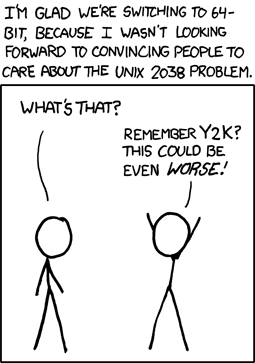
\includegraphics[width=.3\linewidth]{./gfx/xkcd-2038}
	\caption
	[Das \emph{Jahr 2038-Problem}]
	{Das \emph{Jahr 2038-Problem}. Quelle: \url{https://xkcd.com/607/}}
\end{center}
\end{figure}

\subsection{Zeitwerte finden und umrechnen}
Die aktuelle UNIX-Zeit wird von der Funktion \texttt{time} ermittelt. Dieser kann ein Pointer auf ein Objekt vom Typ \mintinline{c}{time_t} übergeben werden, an den die aktuelle Zeit (also die Zahl der Sekunden seit 1970-01-01, 00:00:00) geschrieben werden soll. Alternativ ist auch der Wert \texttt{NULL} als Parameter zulässig -- dann wird kein Wert in den Speicher geschrieben. In beiden Fällen enthält der Rückgabewert die Information der UNIX-Zeit.

\begin{codebox}[Beispiel: \texttt{time}]
\begin{minted}[linenos]{c}
#include <stdio.h>
#include <time.h>

int main () {
  time_t now = time(NULL);
  
  // time(&now);  // alternative Methode
  
  printf("%ld Sekunden seit 1970-01-01, 00:00:00.\n", now);
}
\end{minted}
\end{codebox}

Diese UNIX-Zeit kann nun in \enquote{menschliche Zeitrechnung} übersetzt werden, also in Jahre, Monate, \ldots aufgebrochen werden. Hierzu bedient man sich der Funktion \texttt{gmtime}, die einen Pointer auf ein Ojekt vom Typ \mintinline{c}{time_t} annimmt, und ein Objekt vom Typ \mintinline{c}{struct tm} zurück gibt. Dieser struct ist beschrieben unter \url{https://en.cppreference.com/w/c/chrono/tm} und enthält Felder für Jahr, Monat, Tag, \ldots. Mit \texttt{asctime} kann eine solches Objekt vom Typ 
\mintinline{c}{struct tm} in einen mit \texttt{printf} druckbaren Text umgewandelt werden (siehe \url{https://en.cppreference.com/w/c/chrono/asctime}).

\begin{codebox}[Beispiel: \texttt{time} in ein Datum übersetzen]
\begin{minted}[linenos]{c}
#include <stdio.h>
#include <time.h>

int main () {
  time_t now = time(NULL);
  printf("Now: %s", asctime(gmtime(&now)));
}
\end{minted}
\end{codebox}

\begin{cmdbox}[Ausgabebeispiel: \texttt{time} in ein Datum übersetzen]
Now: Fri Jun 21 19:50:01 2019
\end{cmdbox}

Um Objekte vom Typ \mintinline{c}{struct tm} zu erzeugen, sollte die Funktion \texttt{mktime} verwendet werden (\url{https://en.cppreference.com/w/c/chrono/mktime}). Die Funktion \texttt{strftime} erlaubt außerdem auch die Darstellung in anderen Zeit-Formaten als dem Amerikanischen (\url{https://en.cppreference.com/w/c/chrono/strftime}).

\subsection{Genaue Zeitmessung und Ticks}
Zeitangaben, die im Zusammenhang mit der UNIX-Zeit stehen sind nur auf eine Sekunde genau. Wo Genauigkeit auf unter eine Sekunde (und bis zu Nanosekunden hinab) gefragt ist, kann mit dem Datentyp \mintinline{c}{clock_t} gearbeitet werden. Auch hier handelt es sich um ein Alias für einen Ganzzahl-Datentyp. Mit Objekten dieses Typs werden aber nicht die Sekunden seit der UNIX-Epoche gezählt, sondern die \emph{Prozessortakte} seit einer bestimmten, nicht näher spezifizierten Referenzzeit. Üblichrweise ist diese Referenzzeit der Beginn der Ausführung des Programms.

Kennt man die Zahl der Prozessortakte, die in einer Sekunde umgesetzt werden, kann dies also leicht durch Division in eine Zeitdauer übersetzt werden. Genau diese Information -- Prozessortakte pro Sekunde -- ist in dem Macro \texttt{CLOCKS\_PER\_SEC} zugänglich:

\begin{codebox}[Beispiel: \texttt{clock}]
\begin{minted}[linenos]{c}
#include <stdio.h>
#include <time.h>
 
int main (void) {
  clock_t start = clock();
 
  // Zeitaufwändige Simulation
 
  clock_t end = clock();
  
  double cpu_time_used = ((double) (end - start)) / CLOCKS_PER_SEC; 
  printf("Die Simulation lief für %df Sekunden.\n", cpu_time_used);
}
\end{minted}
\end{codebox}

\subsection{Kurze Wartezeiten}
Manchmal möchte man den Ablauf seines Programms absichtlich verzögern. Dies könnte beispielsweise der Fall sein, wenn Sie ein Spiel programmieren, in dem Sie Ihren Spielern nicht Reaktionsvermögen einer CPU abverlangen wollen. 

Zu diesem Zweck existiert die Funktion \texttt{nanosleep}, die im POSIX-Standard von 1993 definiert wurde. Der Standard kann als Erweiterung zum C-Standard aufgefasst werden. Befehle, die hiervon abgedeckt werden gehören nicht mehr zum normalen Sprachumfang und werden nicht alleine durch Einbinden der richtigen Bibliotheken frei geschalten. Stattdessen muss eine Präprozessor-Konstante \texttt{\_POSIX\_C\_SOURCE} dem Compiler mitteilen, dass diese erweiterten Funktionen mit beachtet werden sollen\footnote{Im Header \texttt{<time.h>} finden Sie ein \mintinline{c}{#if}, das dafür sorgt, dass einige Definitionen nur umgesetzt werden, wenn die Präprozessor-Konstante einen geeigneten Wert hat.}.

Sobald \texttt{nanosleep} in Ihrem Code verfügbar gemacht wurde, können Sie es nach folgendem Beispiel benuzen:

\begin{codebox}[Beispiel: \texttt{clock}]
\begin{minted}[linenos]{c}
#define _POSIX_C_SOURCE 199309L   // this enables nanosleep
#include <time.h>

void   wait_ms(unsigned long miliseconds) {
  struct timespec sleeptime;
  
  if(miliseconds > 999) {   
    sleeptime.tv_sec  = (int) (miliseconds / 1000);
    sleeptime.tv_nsec = (miliseconds 
                      - ((long) sleeptime.tv_sec * 1000)) * 1000000;
  } else {   
    sleeptime.tv_sec = 0;
    sleeptime.tv_nsec = miliseconds * 1000000;
  }
  
  nanosleep(&sleeptime, NULL);
}
\end{minted}
\textrm{(Quelle:} \url{https://stackoverflow.com/questions/7684359}\textrm{)}
\end{codebox}

Eine genaue Beschreibung des Befehls finden Sie unter \url{http://man7.org/linux/man-pages/man2/nanosleep.2.html}

\begin{hintbox}[Es gäbe noch mehr zu sagen \ldots]
In diesem Abschnitt sollte Ihnen nur ein Überblick in die Logik hinter der time-library gegeben werden. Ich ermutige Sie also, selbstständig die unter \url{https://en.cppreference.com/w/c/chrono} aufgelisteten Funktionen selbstständig zu erkunden.
\end{hintbox}

\section{Zufallszahlen} \label{sec:RandomNums}
Computer sind \emph{deterministische} Maschinen. Das bedeutet, dass alle Ergebnisse, die mit einem Computer gewonnen werden können, bereits durch seinen Ausgangszustand vorgegeben sind. Kennt man den gesamten Speicherinhalt eines Rechners, so lässt sich daraus das Ergebnis jeder Berechnung und jedes Algorithmus ableiten. Dies schließt somit \emph{Zufall} bereits vollkommen aus.

Während \emph{echter} Zufall einem Computerprogramm nicht zugänglich ist, können wir aber zumindest Zahlenreihen erzeugen, die zufällig \emph{wirken}. Es ist einem Menschen \idR nicht möglich, die nächste Zahl einer solchen \emph{Pseudozufahlsreihe} vorherzusagen. In der Regel sind solche Zufallsreihen \emph{rekursiv} definiert, \ie eine Pseudozufallszahl wird aus ihrem Vorgänger berechnet. Damit gilt wieder, dass mit der ersten Zahl die komplette Zufallsreihe vorherbestimmt ist. Durch geschickte Wahl des Startwerts kann man aber echtem Zufall für die praktische Anwendung nahe genug kommen.

Im Header \texttt{<stdlib.h>} sind die Funktionen \texttt{rand} und \texttt{srand} deklariert, die zu diesem Zweck dienen. 
\begin{description}
\item[\texttt{rand}] gibt die nächste Zahl einer Zufallsreihe aus. Berechnet wird eine positive Ganzzahl zwischen 0 und \texttt{RAND\_MAX}. Letzteres wiederum ist ein Symbol, das ebenfalls in \texttt{<stdlib.h>} definiert ist, und dessen Wert von der Version des Compilers abhängt. I.\,d.\,R. handelt es sich um die größte Zahl, die mit dem Datentyp \mintinline{c}{int} dargestellt werden kann.
\item[\texttt{srand}] legt den Startwert fest. Als Argument wird eine vorzeichenlose Ganzzahl erwartet.
\end{description}

Es bietet sich an, als Startwert beispielsweise die aktuelle Systemzeit zu verwenden, wie sie von \texttt{time} zurück gegeben wird. Da dieser Wert im Allgemeinen bei jeder Programmausführung ein anderer ist, erhält man einen für praktische Zwecke gut geeigneten Pseudo-Zufallsgenerator.

In der praktischen Anwendung kann dies so aussehen:
\begin{codebox}[Beispiel: Pseudozufallszahlen]
\begin{minted}[linenos]{c}
#include <stdio.h>
#include <stdlib.h>
#include <time.h>

int main () {
  srand(time(NULL));      // "zufälligen" Startwert wählen
  
  printf("drei zufällige Ganzzahlen:\n");
  for (int i=0; i<3; i++) {
    printf("%d\n", rand());
  }
  
  printf("\ndrei zufällige Ganzzahlen zwischen 0 und 5:\n");
  for (int i=0; i<3; i++) {
    printf("%d\n", rand() % 6);
  }
  
  printf("\ndrei zufällige Fließkommazahlen zwischen 0 und 1:\n");
  for (int i=0; i<3; i++) {
    printf("%lf\n", (double) rand() / RAND_MAX);
  }
\end{minted}
\end{codebox}
%
\begin{codebox}[]
\begin{minted}[linenos, firstnumber=last]{c}
  
  double lo = 5;
  double hi = 15;
  printf("drei zufällige Fließkommazahlen zwischen %lf und %lf:\n", lo, hi);
  for (int i=0; i<3; i++) {
    printf("%lf\n", lo + ((double) rand() / RAND_MAX) * (hi-lo));
  }
}
\end{minted}
\end{codebox}

\begin{cmdbox}[Ausgabebeispiel: Zufallszahlen]
\begin{minted}{text}
drei zufällige Ganzzahlen:
1726242556
1893651755
1463512462

drei zufällige Ganzzahlen zwischen 0 und 5:
3
1
1

drei zufällige Fließkommazahlen zwischen 0 und 1:
0.662454
0.426405
0.427842

drei zufällige Fließkommazahlen zwischen 5.000000 und 15.000000:
5.544294
5.964819
9.742072
\end{minted}
\end{cmdbox}

\begin{hintbox}[Linear Congruential Generator -- der C-Standard-Pseudozufallsgenerator]
Der C-Standard schreibt nicht vor, wie der Algorithmus hinter \texttt{rand} genau auszusehen hat. Üblicherweise wird aber ein \emph{Linear Congruential Generator} implementiert. Diese funktionieren nach dem Prinzip:
\[ x_i = (a x_{i-1} + c) \mod m \]
Hierbei sind $x_i$ die berechneten Pseudozufallszahlen, \ie $x_{i-1}$ steht für den Vorgänger der gerade berechneten Zahl. Die Parameter $a$, $c$ und $m$ sind mehr oder minder beliebige Konstanten. Der Wert von $m$ legt den größten Wert fest, den diese Methode generieren wird. Eine geschickte Wahl von $a$ und $c$ sorgen für eine möglichst gleichmäßige Verteilung der Zufallswerte.

Der \texttt{gcc} verwendet:
\begin{align*}
	m &= 2^{31}\\
	a &= 1\,103\,515\,245\\
	c &= 12345
\end{align*}
(Siehe \url{https://en.wikipedia.org/wiki/Linear_congruential_generator})
\end{hintbox}

\begin{warnbox}[Statistische Qualität von Zufallszahlen]
Für allgemeine Anwendungen -- etwa die Programmierung von Spielen -- genügt der Standard-Zufallsgenerator des \texttt{gcc} vollkommen. Zu wissenschaftlichen Simulationen aber ist dieser \emph{nicht geeignet}. Die einzelnen Werte sind noch zu stark korrelliert, und die Periode (\ie die Zahl von Zufallswerten, bevor sich die Wertereihe wiederholt) ist zu gering.

Für Wissenschaftliche Arbeiten stehen viele Bibliotheken zur Verfügung, die ausgereiftere (aber auch langsamer arbeitende) Pseudozufalls-Generatoren anbieten. Ein Beispiel hierfür ist die \emph{Gnu Scientific Library} (GSL).

Siehe \url{https://www.gnu.org/software/gsl/}
\end{warnbox}

\section{\texttt{nan} -- not a number} \label{sec:NAN}
Fließkommazahlen -- also \mintinline{c}{float}s und \mintinline{c}{double}s -- haben eine interessante Eigenschaft: Sie können auch mathematische Objekte darstellen, die streng genommen \emph{keine Zahlen} sind. Bestimmte Bitmuster werden nicht als Zahl ausgewertet sondern stehen für das Ergebnis einer fehlerhaften Berechnung wie etwa die Wurzel aus einer negativen Zahl\footnote{C bietet zwar eine Bibliothek zur Arbeit mit komplexen Zahlen an. Für den \enquote{normalen} Betrieb gelten solche Rechnungen aber als nicht lösbar. Siehe dazu auch Abschnitt \ref{sec:complexNums}}. Wir nennen diese Bitmuster \emph{not a number} oder kurz \emph{NAN}.

Je nach Datentyp und Compiler werden unterschiedliche NANs unterschieden. Allen ist gemeinsam, dass jede Fließkomma-Rechnung, an denen eine NAN beteiligt ist, wieder eine NAN gleicher Art erzeugt. Soll eine solche NAN in eine Ganzzahl-Variable übertragen werden, so erzeugt dies, abhängig von Ziel-Datentyp und Compiler, entweder den Wert \texttt{0} oder $-2^{b}$ -- wobei $b$ die Breite des Datentyps in bits ist. Für \mintinline{c}{int}s (32bit) ergibt sich so der Wert \texttt{-2\,147\,483\,648}.

Bei der Ausgabe mit \texttt{printf} werden alle NANs durch die Zeichenkette \texttt{nan} dargestellt:
\begin{codebox}[Beispiel: NANs]
\begin{minted}[linenos]{c}
#include <stdio.h>
#include <math.h>

int main () {
  double nan = sqrt(-1.0);
  
  char         nan_char  = nan;
  short        nan_short = nan;
  int          nan_int   = nan;
  unsigned int nan_uint  = nan;
  long         nan_long  = nan;
  
  printf("nan als double: %lf\n" , nan      );
  printf("nan als char  : %hhd\n", nan_char );
  printf("nan als short : %hd\n" , nan_short);
  printf("nan als int   : %d\n"  , nan_int  );
  printf("nan als uint  : %d\n"  , nan_uint );
  printf("nan als long  : %ld\n" , nan_long );
  
  return 0;
}
\end{minted}
\end{codebox}

\begin{cmdbox}[Ausgabebeispiel: NANs]
\begin{minted}{text}
nan als double: nan
nan als char  : 0
nan als short : 0
nan als int   : -2147483648
nan als uint  : 0
nan als long  : -9223372036854775808
\end{minted}
\end{cmdbox}

Um zu überprüfen, ob ein Fließkommawert ein NAN ist (gleich welcher Art) kann das Macro \texttt{isnan} (definiert im Header \texttt{<math.h>}) benutzt werden:

\begin{codebox}[Beispiel: \texttt{isnan}]
\begin{minted}[linenos]{c}
#include <stdio.h>
#include <math.h>

int main () {
  printf("sqrt(+1.0)     ist %snan\n", (isnan(sqrt(+1.0)    ) ? "" : "kein "));
  printf("sqrt(-1.0)     ist %snan\n", (isnan(sqrt(-1.0)    ) ? "" : "kein "));
  printf("sqrt(-1.0) + 1 ist %snan\n", (isnan(sqrt(-1.0) + 1) ? "" : "kein "));
  
  return 0;
}
\end{minted}
\end{codebox}

\begin{cmdbox}[Ausgabebeispiel: \texttt{isnan}]
\begin{minted}{text}
sqrt(+1.0)     ist kein nan
sqrt(-1.0)     ist nan
sqrt(-1.0) + 1 ist nan
\end{minted}
\end{cmdbox}

Schließlich ist im Header \texttt{<float.h>} die Makro-Konstante \texttt{NAN} definiert, die zur schnellen bzw. klaren Erzeugung eines solchen Fehlerwerts geeignet ist.

\section{\texttt{atexit}}
Manche Aufgaben sollen erst ausgeführt werden, wenn das Programm beendet wird. Dies kann beispielsweise das Schließen von Logfiles sein oder die Freigabe von Speicherbereichen mit \texttt{free}.
Damit wir nicht jeden Pfad, auf den unser Programm enden kann, nachverfolgen müssen, können wir mit der Funktion \texttt{atexit} (deklariert im Heaer \texttt{<stdlib.h>}) eine oder mehrere eigene Funktionen registrieren, die bei Ende unseres Programms aufgerufen werden sollen.

Als Parameter wird ein Funktionszeiger auf eine \mintinline{c}{void}-Funktion ohne Parameter erwartet. (Da bei Programmende keine Stelle mehr einen Rückgabewert empfangen kann, ist der Rückgabetyp \mintinline{c}{void} naheliegend. Bedingt durch den automatischen Aufruf können auch keine Parameter übergeben werden. Werden in der Funktion dennoch zusätzliche Informationen gebraucht, muss dies über globale Variablen gelöst werden.)

\begin{codebox}[Beispiel: \texttt{atexit}]
\begin{minted}[linenos]{c}
#include <stdio.h>
#include <stdlib.h>

FILE * hDebug = NULL;

void handler_quit () {
  if (hDebug) {
    fclose(hDebug);
    printf("Debug Log geschlossen.\n");
  }
}

int main () {
  atexit(handler_quit);
  hDebug = fopen("debuglog.txt", "w");
  
  // restlicher Code...
}
\end{minted}
\end{codebox}


\section{Variadische Funktionen}
Wie wir wissen, können die Funktionen \texttt{printf} und \texttt{scanf} beliebig viele Parameter entgegen nehmen. Dies ist möglich, indem sie als \emph{variadische Funktionen} deklariert sind. Das bedeutet, dass ihre Signatur nur eine gewisse Anzahl an festen Parametern vorsieht und danach durch drei Punkte angedeutet wird, dass hier beliebige Werte folgen dürfen:

\begin{codebox}[Syntax: Prototyp einer variadischen Funktion]
\begin{minted}{c}
Rückgabetyp Funktionsname (Parameterliste_fest, ...);
\end{minted}
\end{codebox}

Um auf die so übergebenen \emph{variadischen Parameter} zuzugreifen, bietet der Header \texttt{<stdarg.h>} einge Macros an über die geeignete Pointer erhalten werden können.

Um die variadischen Parameter auszulesen benötigen wir zunächst ein Objekt vom Typ 
\mintinline{c}{va_list}, das als Handle auf die Parameter fungiert. Im folgenden soll diese Variable \texttt{args} genannt werden.

\texttt{args} wird über das Macro \mintinline{c}{va_start} initialisiert, dem wir dazu \texttt{args} als ersten Parameter übergeben mussen und zusätzlich den letzten Parameter, der \enquote{regulär} an unsere variadische Funktion übergeben wurde.

Einmal initialisiert liest das Macro \mintinline{c}{va_arg} nun aus \texttt{args} Werte beliebigen Typs aus. Als Parameter wird \texttt{arg} sowie der Datentyp des nächsten zu lesenden Wertes übergeben.
Ist die Arbeit mit der Liste beendet, muss mit \mintinline{c}{va_end} Speicher freigegeben werden.

Dieses abstrakte Vorgehen wird klarer, wenn wir ein Beispiel aus der CPP-Referenz betrachten:

\begin{codebox}[Beispiel: Variadische Funktion zum Aufsummieren beliebig vieler \texttt{int}s]
\begin{minted}[linenos]{c}
#include <stdio.h>
#include <stdarg.h>
 
int add_nums(int count, ...) {
  int result = 0;
  
  va_list args;                   // Liste variadischer Parameter
  va_start(args, count);          // Liste vorbereiten, Startpunkt nach count
  
  for (int i = 0; i < count; ++i) {
    result += va_arg(args, int);  // int-Werte aus der Liste lesen
  }
  
  va_end(args);
  return result;                  // Handle auf variadische Liste freigeben
}
 
int main() {
  printf("%d\n", add_nums(4, 25, 25, 50, 50));
}
\end{minted}
\end{codebox}

Besteht die variadische Liste aus Parametern unterschiedlichen Typs, so müssen die festen Parameter die Information enthalten, welche Datentypen an welcher Stelle der Liste stehen. Üblicherweise geschieht dies über einen \emph{Format String}. Die Interpretation eines solchen Strings nennt man auch \emph{parsen}.

\section{Komplexe Zahlen} \label{sec:complexNums}
Im Kontext von naturwissenschaftlichen Simulationen kommen häufig auch Rechnungen mit komplexen Zahlen vor. Der Header \texttt{<complex.h>} stellt einige Deklarationen und Makros bereit, die die Arbeit hiermit erleichtern.

Sobald der Header eingebunden ist, stehen die neuen Datentypen \mintinline{c}{complex float}, \mintinline{c}{complex double} und \mintinline{c}{complex long double} zur Verfügung. Wie ihre \enquote{Cousins} in den reellen Zahlen unterscheiden sich die drei Datentypen in der \emph{Rechengenauigkeit}, also in der Zahl der signifikanten Ziffern, die zur Verfügung stehen.

Mit Ausdrücken vom Typ \mintinline{c}{complex XXX} können die vier Grundrechenarten direkt mit den bekannten Operatoren (\texttt{+}, \texttt{-}, \texttt{*}, \texttt{/}) durchgeführt werden. Auch hier werden die gängigen Rechenregeln (Punkt vor Strich, Behandlung von Real- und Imaginärteil, \ldots) beachtet.

Der Header \texttt{<complex.h>} definiert auch das Symbol \texttt{I}, mit dem die imaginäre Einheit dargestellt wird. Mit den Funktionen \texttt{creal} und \texttt{cimag} kann der Real- bzw. Imaginärteil eines Ausdrucks vom Typ \mintinline{c}{complex XXX} ausgelesen werden.

Damit funktioniert dann der folgende Code:

\begin{codebox}[Beispiel: Grundrechenarten mit komplexen Zahlen]
\begin{minted}[linenos]{c}
#include <stdio.h>
#include <complex.h>

 
int main() {
  complex double z1 = 1.0 + 2.0 * I;
  complex double z2 = 5.0 - 2.7 * I;
  
  complex double z3 = z1 * z2 + z1;
  
  printf("Ergebnis: %lf%+lfi\n", creal(z3), cimag(z3));
}
\end{minted}
\end{codebox}

\begin{cmdbox}[Ausgabebeispiel: Grundrechenarten mit komplexen Zahlen]
Ergebnis: 11.400000+9.300000i
\end{cmdbox}

Für die wichtigsten aufwändigeren Operationen (Wurzel, Exponentialfunktion, Logarithmus, trigonometrische Funktionen, ...) existieren Analoga zu den bekannten Funktionen, die mit komplexen Zahlen funktionieren. Diese Funktionen haben denselben Namen wie die aus der \texttt{<math.h>} bekannten Routinen, beginnen aber mit dem Präfix \texttt{c}. Das bedeutet \eg, dass die Funktion \texttt{csin} den Sinus einer komplexen Zahl berechnet.

Um diese Funktionen benutzen zu können muss (wie auch schon bei den reellen mathematischen Funktionen) gegen die math-library gelinkt werden. Das heißt, der Compiler muss mit der Kommandozeilenoption \texttt{-lm} gestartet werden.

\begin{codebox}[Beispiel: Funktionen mit komplexen Zahlen]
\begin{minted}[linenos]{c}
#include <stdio.h>
#include <complex.h>
 
int main() {
  const int    lines     = 20;
  const double offset    = 40.0;
  const double height    = 10.0;
  const double frequency =  0.5;
  
  complex double result;
  
  for (int i=0; i<lines; i++) {
    result = cexp(i * frequency * I);
    
    for (int j=0; j<offset + creal(result) * height; j++) {
      printf(" ");
    }
    printf("*\n");
  }
}
\end{minted}
\end{codebox}

\begin{cmdbox}[Ausgabebeispiel: Funktionen mit komplexen Zahlen]
\begin{minted}{text}
                                                  *
                                                 *
                                              *
                                         *
                                    *
                                *
                               *
                               *
                                  *
                                      *
                                           *
                                                *
                                                  *
                                                  *
                                                *
                                            *
                                       *
                                  *
                               *
                               *
\end{minted}
\end{cmdbox}

Siehe \url{https://en.cppreference.com/w/c/numeric/complex} für eine Übersicht der komplexen Funktionen.

\section{Debugger}
Bis zu diesem Punkt haben Sie sicher schon festgestellt, wie häufig die ersten Zeilen Code, die wir schreiben fehlerhaft sind und nicht das Ergebnis erzielen, das wir uns erhoffen. Je größer und komplexer unsere Projekte werden, desto schwieriger wird es auch, einen Fehler ausfindig zu machen und zu korrigieren. Die Schwierigkeit besteht darin, die Entwicklung von den vielen Variablen nachzuverfolgen, mit denen wir arbeiten.

Um diese Aufgabe zu erleichtern steht das Tool \texttt{gdb} (GNU debugger) zur Verfügung. Das Programm wird von der Kommandozeile aufgerufen und bietet einen gewissen Einblick in unser laufendes Programm. Damit der Debugger diesen Einblick gewähren kann, müssen wir dem Compiler allerdings mitteilen, dass beim Übersetzen in Maschinensprache die Variablennamen und andere Informationen über unseren Quellcode erhalten bleiben sollen. Dies erreichen wir, indem wir den Compiler mit der Kommandozeilenoption \texttt{-g} aufrufen.

\begin{hintbox}[Performanz]
Programme, die mit der Debug-Option \texttt{-g} kompiliert wurden sind größer und laufen langsamer. Während der Entwicklung ist es sinnvoll, die Option zu nutzen, um eben den Support des \texttt{gdb} nutzen zu können. Vergessen Sie jedoch nicht, die finale Version ohne diese Option zu kompilieren, um das Maximum an Leistungsfähigkeit herauszuholen.
\end{hintbox}

Wenn Sie den \texttt{gdb} starten, finden Sie sich in einer neuen Kommandozeilen-Umgebung wieder. Das bedeutet, dass Sie, wie auch bei der Linux-Konsole, Kommandos eingeben und mit ENTER bestätigen können. Diese Kommandos sind jetzt jedoch andere, als dies in der normalen Konsole wäre.

Als ersten Schritt in der \texttt{gdb}-Umgebung können Sie mit dem folgenden Befehl festlegen, welches Programm Sie debuggen wollen:
\begin{cmdbox}[gdb: Programm festlegen]
file <executable>
\end{cmdbox}
Dabei steht \texttt{<executable>} für den Dateinamen Ihres \emph{ausführbaren} Programms. In den vorigen Beispielen wäre das also jeweils \texttt{./myProgram} gewesen.

Der Befehl \texttt{run} führt Ihr Programm aus. Sie können auch Kommandozeilenparameter an Ihr Programm übergeben, indem Sie diese hinter \texttt{run} setzen:
\begin{cmdbox}[gdb: Programm mit Kommandozeilenarametern starten]
run param1 param2 ...
\end{cmdbox}

Sie können im Vorfeld Punkte festlegen, an denen die Ausführung des Programms pausiert werden soll. Dies geschieht mit dem Befehl \texttt{break}. Hinter \texttt{break} können Sie entweder einen Funktionsnamen oder eine Zeilennummer angeben.

Ist ein solcher \emph{Breakpoint} erreicht, kann mit \texttt{print} der Wert von Variablen ausgegeben werden. Der folgende Befehl wird beispielsweise den Wert der Variablen \texttt{x} im aktuellen Zustand des Programms ausgeben:
\begin{cmdbox}[gdb: Wert von Variablen ausgeben]
print x
\end{cmdbox}

Schließlich lässt sich mit \texttt{continue} die Ausführung fortsetzen. Das Programm läuft weiter, bis ein neuer Breakpoint erreicht wird, bis das Programm regulär zu seinem Ende kommt oder bis es abstürzt.

Unter \url{https://web.eecs.umich.edu/~sugih/pointers/summary.html} finden Sie weitere Details zum GNU-Debugger.

\begin{hintbox}[Weitere Features]
Aus Gründen der Übersichtlichkeit können hier nur die wichtigsten Features des gdb vorgestellt werden. Dies soll aber nicht den Eindruck erwecken, dass der Funktionsumfang des Debuggers komplett durch einige zusätzliche \texttt{printf}-Zeilen im Code ersetzt werden könnte.
Lesen Sie beispielsweise unter \url{https://www.cs.umd.edu/~srhuang/teaching/cmsc212/gdb-tutorial-handout.pdf} über weitere Features des \texttt{gdb}.
\end{hintbox}
%
%\section{Die Bibliothek ncurses}
%
%\url{http://www.tldp.org/HOWTO/NCURSES-Programming-HOWTO/}
%	\include{16_Recursion}
%	\include{17_LinkedLists}
%	\include{18_CPP}
%
	\appendix
\begin{appendices}
\chapter{Begriffe}
\section*{A...}
\begin{description}
\item[Adresse] \enquote{Nummer des Bytes im Speicher}, ab dem eine Information zu finden ist.\newline
	Siehe Abschnitt \ref{sec:Pointer}
\item[Adress-Operator] Das Zeichen \texttt{\&}. Wird vor Variablen gestellt, um den Speicherort (\ie die 
	\emph{Adresse}) der Variable zu ermitteln.\newline
	Siehe Abschnitt \ref{sec:Pointer}
\item[Allozieren] Anfrage an das Betriebssystem, einen Speicherbereich für andere Programme zu sperren,
	also den Speicherbereich für eine bestimmte Aufgabe zu \emph{reservieren}. Üblicherweise mit den 
	Befehlen \texttt{malloc} oder \texttt{calloc} aus dem \emph{Header} \texttt{<stdlib.h>} umgesetzt.
	\newline
	Siehe Abschnitt \ref{sec:allocation}
\item[Alphanumerisch] Schriftzeichen, die für menschliche Worte (im Englischen) üblich sind, sowie
	Ziffern: A-Z, a-z, 0-9.
\item[Argument] Wert, der einer \emph{Funktion} in runden Klammern \texttt{()} \emph{übergeben} wird.
	Die Funkion kann nun mit diesem Wert arbeiten. Argumente können \emph{Konstanten}, \emph{Variablen}
	oder komplexe \emph{Ausdrücke} sein.\newline
	Beispiel: Die Funktion \texttt{sin} erwartet ein \emph{Argument} vom \texttt{Datentyp} 
	\mintinline{c}{double}. Damit können als Argumente \eg \texttt{0}, \texttt{x} oder 
	\texttt{3.14 * x + acos(0)} möglich.\newline
	Siehe Abschnitt \ref{sec:funcs}
\item[Array] Eine Liste von Werten, die im Speicher \enquote{hintereinander} abgelegt wird. Zugriff auf
	die Elemente des Arrays geschieht über einen \emph{Pointer} auf den Listenanfang und einen
	\emph{Index}.\newline
	Siehe Abschnitt \ref{sec:Arrays}
\item[Assembler] Eine Programmiersprache und auch der Name einer Art von Programmen.\newline
	Die Befehle der Sprache Assembler entsprechen dem (sehr kleinen) Befehlssatz eines Prozessors. Daher
	ist in dieser Sprache eine sehr hardwarenahe, kleinschrittige Denkweise notwendig.\newline
	\emph{Hochsprachen} erlauben größere Abstraktion und dadurch eine für Menschen natürlichere
	Denkweise. Oft werden Hochsprachen-Programme erst in die Sprache Assembler übersetzt und dann von
	einem Assembler-Programm in \emph{Maschinensprache} weiter übersetzt.\newline
	Siehe Abschnitt \ref{sec:assembly}
\item[Ausdruck] Eine Folge von \emph{Konstanten}, \emph{Variablen} und \emph{Funktionsaufrufen}, die
	durch \emph{Operatoren} so miteinander verknüpft sind, dass daraus ein Wert berechnet werden kann.
	\newline
	Beispiele (jeweils durch Semikolons getrennt): \texttt{x + 9}; \texttt{42}; 
	\texttt{-sqrt(5.3) * 7 - y}; \texttt{x > y}.\newline
	Siehe Abschnitt \ref{chp:expressions}
\item[Ausschlussset-Schreibweise] Teil eines \emph{Format-Strings} bei \texttt{scanf}, der bei der
	Eingabe von \emph{Strings} benutzt wird. Form \mintinline{c}{[^...]}, wobei \texttt{...} für die
	Zeichen steht, die \emph{nicht} beachtet werden sollen.\newline
	Siehe Abschnitt \ref{sec:strInput}
\item[Automatische Arrays] \emph{Arrays}, die vom Compiler verwaltet werden, \ie für die kein
	Speicher mit \texttt{malloc} \emph{alloziert} werden muss, und die nicht mit \texttt{free}
	freigegeben werden dürfen. Bei der \emph{Deklaration} wird in [eckige Klammern] die Arraygröße in
	Elementen angegeben (Ausnahme: \emph{Initializer-List}).\\
	Einmal angelegt kann die Größe von automatischen Arrays nicht mehr geändert werden. Siehe daher auch 
	\emph{Dynamische Arrays}, die zur \emph{Laufzeit} die Größe ändern können\\
	Siehe Abschnitt \ref{sec:Arrays}

\section*{B...}
\item[Bibliothek] Eine Sammlung von \emph{Routinen}, die für sich genommen kein alleinstehendes Programm
	ergeben, die aber Probleme lösen, welche in anderen Programmen (mehrfach) auftreten können.
	Üblicherweise stehen Bibliotheken als \emph{vorkompilierte} Datenobjekte zur Verfügung. Sie werden
	über einen \emph{Header} in den eigenen Code eingebunden. Beim \emph{kompilieren} muss gegen die
	Bibliothek \emph{gelinkt} werden.\newline
	Siehe Abschnitt \ref{sec:Compile} und Kapitel \ref{chp:modules}
\item[Binärformat] Darstellung von Werten in einem Format, das von Computern leicht und effizient
	verarbeitet werden kann, das für Menschen dagegen idR nicht entzifferbar ist. Dateien in diesem
	Format werden mit \texttt{fwrite} geschrieben und mit \texttt{fread} gelesen. Alle Werte im Speicher
	werden im Binärformat gehalten.\newline
	Siehe Abschnitt \ref{sec:binAccess}
\item[Binärsystem] Zahlensystem, das lediglich aus den Ziffern \texttt{0} und \texttt{1} besteht und die
	Grundlage der Rechner-Elektronik bildet. \newline
	Siehe Abschnitt \ref{sec:BinaryNumbers}
\item[Bitweise Operatoren] \emph{Operatoren}, die nicht mit Zahlen als Einheit arbeiten, sondern die die
	einzelnen Bits der Zahlen getrennt voneinander verarbeiten. Die Bitweisen Operatoren werden
	mit den Zeichen \texttt{\textasciicircum}, \texttt{\&}, \texttt{|} und \texttt{\^} gesetzt und sind
	von den \emph{logischen Operatoren} abzugrenzen.\newline
	Siehe Abschnitt \ref{sec:BitwiseOperator}

\section*{C...}
\item[Compiler] Ein Programm, das die Übersetzung von (menschenlesbarer) Programmiersprache in
	\emph{Maschinensprache} übernimmt. Häufig wird dabei zunächst als Zwischenschritt in
	\emph{Assembler} \emph{transpiliert}.\newline
	Umgangssprachlich wird das \emph{Linken} auch als Teil des Kompilier-Vorgangs aufgefasst.\newline
	Siehe Abschnitt \ref{sec:Compile}.
	
\section*{D...}
\item[Dateimodi] Lese- oder Schreibzugriff.\\
	Siehe Abschnitt \ref{sec:fileAccess}
\item[Datentyp] Die Art der Information, auf die über eine \emph{Variable} oder einen \emph{Ausdruck} 
	zugegriffen werden kann, bzw. die einer \emph{Konstanten} zugeordnet ist. Ein Datentyp kann eine von
	mehreren Arten von \emph{Ganzzahlen}, \emph{Fließkommazahlen} oder \emph{Pointern} sein.\\
	Siehe Abschnitt \ref{chp:expressions} sowie die Tabellen \ref{tab:DatatypesStd} und
	\ref{tab:DatatypesExt}
\item[Definition] Eine Anweisung, die zwar die Bedeutung eines Symbols festlegt, aber keine
	\emph{Speicherstelle} reserviert oder ändert.\\
	Siehe \emph{Forward declaration}, \emph{Header}, \emph{Präprozessor}.
\item[Deklaration] Abschnitt im Code, bei dem einem \emph{Symbol} innerhalb seines Scopes eine
	ein \emph{Datentyp} und eine \emph{Speicherstelle} zugewiesen werden (letzteres geschieht dabei
	automatisch).\\
	Siehe Abschnitte \ref{sec:DeclareVars} und \ref{sec:funcs}
\item[Dereferenzierung] Anweisung an den Compiler, nicht mit einem \emph{Pointer} zu arbeiten, sondern
	mit dem Wert im Speicher, der durch den Pointer referenziert wird. Dies geschieht entweder über den
	Dereferenzierungsoperator (\texttt{*pointer}) oder über den Array-Index-Zugriff
	(\texttt{pointer[index]})\\
	Siehe Abschnitte \ref{sec:Pointer} und \ref{sec:Arrays}.
\item[Dualsystem] Synonym für \emph{Binärsystem}
\item[Dynamische Arrays] \emph{Arrays}, die vom/von der ProgrammiererIn verwaltet werden, \ie für die
	Speicher mit \texttt{malloc} \emph{alloziert} werden muss, und die nicht mit \texttt{free}
	freigegeben werden müssen. Bei der \emph{Deklaration} wird das Symbol \texttt{*} benutzt, um
	das zugeordnete Symbol als \emph{Pointer} zu markieren.\\
	\emph{Dynamische Arrays} können zur \emph{Laufzeit} die Größe ändern, sind aber aufwändiger zu
	verwalten als \emph{Automatische Arrays}\\
	Siehe Abschnitt \ref{sec:Arrays}

\section*{E...}
\item[Errorcode] Eine \emph{Ganzzahl} zwischen 0 und 255, die eine Information darüber enthält, welche
	Fehler bei der Ausführung eines Programms aufgetreten sind.\\
	Siehe Abschnitt \ref{sec:errorcodes}
\item[Escape-Char, Escape-Sequenz] Ein Zeichen, das angibt, dass das oder die folgenden Zeichen eines
	Textes nicht eins zu eins umgesetzt werden sollen, sondern durch andere, schwer einzugebende Zeichen
	ersetzt	werden sollen (\eg Zeilenumbruch). In C ist das Escape-Char der Backslash
	\texttt{\textbackslash}.\\
	Escape-Char und \emph{Escape-Sequenz} werden zusammen durch eine Entsprechung ersetzt.\\
	Siehe Tabelle \ref{tab:Escape}
\item[Expansion] Der Code, der vom \emph{Präprozessor} erzeugt wird, nachdem ein \emph{Macro} durch
	seinen Macrotext ersetzt wurde.\\
	Siehe Kapitel \ref{chp:Preprocessor}

\section*{F...}
\item[Fließkommazahl] Eine Information, die eine Zahl mit Nachkomma-Anteil beschreibt, also \eg
	\texttt{3.14} oder auch \texttt{42.0}.\\
	Siehe Abschnitt \ref{sec:valueAssignment}
\item[Format-String] Eine Zeichenkette, die mit \texttt{printf}, \texttt{scanf} und den damit
	verwandeten Funktionen (\texttt{sprintf}, \texttt{fprintf}, \ldots) verwendet wird.\\
	Ein Format-String enthält Steuer-zeichenketten, die über Datentyp und Format von Werten informieren. 
	Diese Zeichenketten beginnen in der Regel mit einem Prozentsymbol \% und können aus einem oder 
	mehreren weiteren Zeichen bestehen.\\
	Siehe Tabellen \ref{tab:FormatOutNum}, \ref{tab:FormatOutSpc} und \ref{tab:FormatIn}
\item[Forward Declaration] Eine \enquote{unvollständige \emph{Deklaration}}, die notwendig ist, um
	Zirkelbezüge aufzulösen. Diese Technik kann mit \emph{Funktionen} und \emph{\mintinline{c}{struct}}s
	angewandt werden.\\
	Siehe Abschnitt \ref{sec:forwardDeclaration} und \ref{sec:typedef}
\item[Function-Body] Die eigentlichen Anweisungen, wie sie bei \emph{Funktionsaufruf} ausgeführt werden,
	eingefasst von \{geschweiften Klammern\}.\\
	Siehe Abschnitt \ref{sec:funcs}
\item[Funktion, Function] Ein Codeabschnitt, der einen eigentständigen \emph{Scope} definiert und eine
	allgemeine Lösung für ein Problem bereitstellt. Funktionen haben einen Namen, einen
	\emph{Rückgabetyp} und eine \emph{Parameterliste} (\ie null bis meherere \emph{Argumente}).\\
	Siehe Abschnitt \ref{sec:funcs}
\item[Funktionsaufruf] Der Befehl, mit der Code-Ausführung in eine \emph{Funktion} zu springen.\\
	Siehe Abschnitt \ref{sec:funcs}
\item[Funktionssignatur] Die Gesamtheit der Informationen \emph{Rückgabetyp} plus \emph{Parameterliste},
	ohne den Funktionsnamen. Man kann die Signatur einer Funktion als ihren \emph{Datentyp} auffassen.\\
	Siehe Abschnitt \ref{sec:funcs}

\section*{G...}
\item[Ganzzahl] Eine Information, die eine Zahl ohne Nachkomma-Anteil beschreibt, also \eg
	\texttt{3} oder auch \texttt{-42}.\\
	Siehe Abschnitt \ref{sec:valueAssignment}

\section*{H...}
\item[Header] Eine Code-Datei, die lediglich \emph{Definitionen} enthält: \emph{Funktions-Signaturen}
	ohne \emph{Function-Body}, \mintinline{c}{struct}s, \mintinline{c}{enum}s und 
	\mintinline{c}{typedef}s sowie \emph{Präprozessor-Direktiven}.\\
	Siehe Abschnitt \ref{sec:funcs}, und Kapitel \ref{chp:structs}, sowie \ref{chp:Preprocessor}
\item[Heap] (Großer) Speicherbereich, der dynamisch verwaltet werden kann, \ie in dem ua
	\emph{dynamische Arrays} angelegt werden.\\
	Siehe Abschnitt \ref{sec:HeapStack}
\item[Hexadezimalsystem] Zahlensystem, das aus 16 Ziffern besteht (0, 1, 2, 3, 4, 5, 6, 7, 8, 9, A, B,
	C, D, E, F). Im Programmier- und Elektronik-Umfeld erlaubt dies eine platzsparende und
	übersichtliche Darstellung mancher Zusammenhänge.\newline
	Siehe Abschnitt \ref{sec:NumSystems}
\item[Hochsprache] Sprachen, die (gemessen am Befehlssatz eines Prozessors) komplexere Aufgaben in
	einem gedanklichen Schritt erledigen lassen. C ist noch sehr systemnah, zählt aber bereits als
	Hochsprache. Das Gegenstück bildet \emph{Assembler} mit einer (beinahen) eins-zu-eins-Entsprechung
	von Befehlen der Sprache und erzeugtem \emph{Maschinencode}.\\
	Siehe Abschnitt \ref{sec:assembly}

\section*{I...}
\item[Index] Nummer eines Elements in einer Liste. Indices beginnen in C bei 0!\\
	Siehe Abschnitt \ref{sec:Arrays}
\item[Initializer-List] Eine durch Kommata getrennte Liste von Werten, eingefasst in \{geschweiften
	Klammern\}. Wird zur gleichzeitigen \emph{Deklaration} und Wertzuweisung bei \emph{automatischen
	Arrays} und \mintinline{c}{struct}s gebraucht.\\
	Siehe Abschnitt \ref{sec:arrayInit} und \ref{sec:structInit}
\item[Instanz] Eine Speicherstelle, der ein Datentyp zugeordnet ist. Dieser Datentyp kann ein
	\emph{primitiver Datentyp} sein oder ein \mintinline{c}{struct}. Die Instanz ist also eine
	\emph{Variable} oder ein \emph{Array}-Element.\\
	Siehe Kapitel \ref{chp:structs}
\item[Iteration, Iterationsschritt] Wiederholung von ähnlichen Vorgängen in direkter Folge, häufig bei
	Veränderung von nur einer Variablen. Synonym für  \emph{Schleifen}. Ein \emph{Iterationsschritt} ist
	ein einzelner Durchlauf des \emph{Schleifenkörpers}.\\
	Siehe Kapitel \ref{chp:loops}

\section*{K...}
\item[Kommandozeile] Text-basiertes User-Interface, in das Kommandos eingegeben werden können, die vom
	Betriebssystem direkt umgesetzt werden. Im Kurs benutzt zum Aufruf des \emph{Compilers} und zum 
	Starten unserer Programme.\\
	Siehe Abschnitt \ref{sec:Compile}
\item[Kommandozeilen-Option] Teil des Textes, der in die \emph{Kommandozeile} eingegeben wird. Diese
	Optionen werden durch Leerzeichen vom Programmnamen und voneinander abgegrenzt, und beeinflussen
	den Programmablauf.\\
	Siehe Abschnitt \ref{sec:cmdlineParams}
\item[Kompilieren] Der Vorgang, bei dem ein menschenlesbarer Programmcode in Maschinensprache übersetzt
	wird. Umgangssprachlich wird das \emph{Linken} als Teil des Kompilierens aufgefasst.\\
	Siehe \emph{Compiler}, \emph{Linker}
\item[Kompilierzeit] Der Zeitpunkt, zu dem ein Programmcode in Maschinensprache übersetzt wird. Hier
	stehen noch nicht alle Informationen zur Verfügung, die zur \emph{Laufzeit} gegeben sind, \eg
	Usereingaben und damit Speicherbedarf. Dies macht dynamische Programmierung notwendig, also etwa
	\emph{dynamische Arrays}.\\
	Siehe Abschnitt \ref{sec:Arrays}
\item[Konstante] Ein Wert im Programm, der -- auch versehentlich -- nicht mehr geändert werden kann,
	sobald das Programm \emph{kompiliert} wurde. Beispiele: \mintinline{c}{3}, \mintinline{c}{"Dune"}
	
\section*{L...}
\item[Laufzeit] Der Zeitpunkt, an dem ein Programm ausgeführt wird. Hier stehen alle Informationen zur
	Verfügung (Usereingaben, Speicherbedarf, ...), aber es können keine strukturellen Änderungen am Code
	mehr durchgeführt werden, da das Programm bereits \emph{kompiliert} ist.\\
	Siehe Abschnitt \ref{sec:Arrays}
\item[Laufzeitverhalten] Die Beziehung von Zeitbedarf zu Datenmenge, die ein Algorithmus verarbeitet.
\item[Library] Englisch für \emph{Bibliothek}
\item[Linker] Ein Programm, das mehrere Dateien mit Code in \emph{Maschinensprache} zu einer einzigen,
	ausführbaren Datei zusammen fügt.
\item[Logische Operatoren] Operatoren, die mit \emph{Wahrheitswerten} operieren. In C existieren die
	logischen Operatoren \texttt{\&\&}, \texttt{||} und \texttt{!}.\\
	Siehe Abschnitt \ref{sec:OperatorsLogical}

\section*{M...}
\item[Macro, Makro] Textblöcke, die vom \emph{Präprozessor} durch anderen Text (Code) ersetzt werden.\\
	Siehe \emph{Expansion}, Kapitel \ref{chp:Preprocessor}
\item[Maschinensprache] Folge von Zahlenwerten, die Anweisungen für den Prozessor enthalten, und die
	vom Menschen nicht mehr (mit vertretbarem Aufwand) verstanden werden können. Wird beim
	\emph{kompilieren} erzeugt.\\
	Siehe Abschnitt \ref{sec:Compile}.
\item[Memory Leakage] Fehler in der Programmierung, bei der \emph{allozierter Speicher} nach
	Programmende nicht mehr freigegeben wird.\\
	Siehe Abchnitt \ref{sec:allocation}
\item[Menschenlesbares Format] Eine Darstellung von Information in für Menschen gedachte Schriftzeichen,
	Insbesondere durch die ASCII-Zeichen 32 bis 127. Daten im Menschenlesbaren Format sind idR weniger
	effizient von Computern erfassbar als solche im \emph{Binärformat}.
\item[Modul] Eine Code-Einheit, die üblicherweise in einer einzelnen Datei abgelegt wird, und zunächst
	zu einem eigenständigen Object-File umgesetzt wird. Code eines Moduls \enquote{lebt} in einem
	eigenen Scope.\\
	Siehe Kapitel \ref{chp:modules}
\item[Modulo-Operator] Berechnet den Rest einer Division. Ausgedrückt durch das Prozent-Symbol \%.\\
	Siehe Abschnitt \ref{sec:OperatorsArithmetic}

\section*{N...}
\item[NAN] \enquote{not a number}. Ein Bitmuster, das bei \emph{Fließkommazahlen} als
	\enquote{Fehlerwert} gedeutet wird. Rechnungen, an denen eine NAN Anteil hat, haben zum Ergebnis
	wiederum eine NAN.
\item[Null-Char] Der Wert \mintinline{c}{0}, als \mintinline{c}{char} im Speicher abgelegt. Dieser Wert
	markiert das Ende eines \emph{Strings}.\\
	Siehe Abschnitt \ref{sec:string}

\section*{O...}
\item[Object-File] Datei bestehend aus \emph{Maschinencode}, der aus einem einzigen \emph{Modul} 
	stammt.\\
	Siehe Abschnitt \ref{sec:Compile}
\item[Offset] Englisch: \enquote{Versatz}: Der Abstand von einem bestimmten Anfangspunkt. Meist der
	Abstand vom Beginn eines \emph{Arrays} zu einer Speicherstelle, gemessen in Bytes; je nach Kontext
	aber auch in der Größeneinheit der Array-Elemente.
\item[Oktalsystem] Zahlensystem, das aus 8 Ziffern besteht (0 \ldots). Im Programmier- und Elektronik-
	Umfeld früher weit verbreitet. Heute nur noch im Kontext von Festplatten-Hardware üblich und
	weitgehend durch das \emph{Hexadezimalsystem} abgelöst\\
	Siehe Abschnitt \ref{sec:NumSystems}
\item[Operator] Eine Rechenanweisung. Wir unterscheiden unäre Operatoren, die nur einen einzigen Wert
	zur Berechnung des Ergebnisses brauchen (\eg. logisches und bitweises NOT, sowie das Vorzeichen
	Minus), binäre Operatoren (die zwei Zahlen brauchen, wie \eg \texttt{+}, \texttt{*}, \texttt{<{}<})
	\\
	Siehe Abschnitte \ref{sec:OperatorsLogical}, \ref{sec:OperatorsArithmetic}
\item[Overhead] Zusätzlicher Verwaltungsaufwand (für den Prozessor), der durch die Nutzung mancher
	Techniken notwendig wird und häufig nicht offensichtlich ist. Beispielsweise muss bei
	\emph{Funktionsaufrufen} der Codepunkt der Fortsetzung nach Funktionsende gespeichert werden,
	\emph{Parameter} kopiert werden und ein Programmsprung ausgeführt werden.

\section*{P...}
\item[Parameter, Parameterliste] Synonym für \emph{Argument}. Eine Parameterliste wird in runden
	Klammern () gesetzt und überhält die Werte, die an eine \emph{Funktion} übergeben werden.\\
	Siehe Abschnitt \ref{sec:funcs}
\item[Parität] Eigenschaft einer ganzen Zahl, gerade oder ungerade zu sein; man sagt also 1 hat ungerade
	Parätät, während 2 gerade Parität hat.
\item[Parsen] Sammelbegriff für das Deuten eines \emph{Strings} in einem bestimmten Kontext, also
	beispielsweise die Zerlegung in einzelne Worte oder die Verarbeitung eines \emph{Format-Strings}.
\item[Pointer] Typ von Variablen, die nicht eine Information selbst, sondern ihre \emph{Adresse} im
	Speicher enthalten.\\
	Siehe Abschnitt \ref{sec:Pointer}
\item[Präprozessor] Ein Programm, das (C-)Code \enquote{vorverarbeitet}, indem bestimmte Text-Elemente
	durch andere ersetzt werden.\\
	Siehe Kapitel \ref{chp:Preprocessor}
\item[Präprozessor-Direktive] Eine Anweisung an den \emph{Präprozessor}, die \eg festlegt, welche
	Ersetzungen vorgenommen werden sollen.
\item[Primitiver Datentyp] Datentypen, wie sie in der Sprache C ohne Zutun des/der ProgrammiererIn zur
	Verfügung stehen.\\
	Siehe Tabellen \ref{tab:DatatypesStd} und \ref{tab:DatatypesExt}
\item[Prototyp] Die erste Zeile einer \emph{Funktion}, in der \emph{Rückgabetyp}, Funktionsname und
	\emph{Parameterliste} zu finden sind.\\
	Siehe Abschnitt \ref{sec:funcs}
\item[Prozedur] Synonym für \emph{Funktion}.\\
	Siehe Abschnitt \ref{sec:funcs}

\section*{R...}
\item[Registerbreite] Die Zahl der Bits, die für eine \emph{Instanz} eines \emph{Datentyps} zur
	Verfügung stehen muss.
\item[Rekursion] Technik, bei der eine Funktion sich selbst aufruft.\\
	Siehe Kapitel \ref{chp:recursion}
\item[Rekursionstiefe] Die \enquote{Anzahl der Verschachtelungen} oder der Aufrufe der \emph{rekursiven}
	\emph{Funktion}\\
	Siehe Kapitel \ref{chp:recursion}
\item[Routine] Synonym für \emph{Funktion}.
\item[Rückgabetyp] Der \emph{Datentyp} des Wertes, der von einer \emph{Funktion} berechnet wird.\\
	Siehe Abschnitt \ref{sec:funcs}
\item[Rückgabewert] Der Wert, der von einer \emph{Funktion} berechnet wird.\\
	Siehe Abschnitt \ref{sec:funcs}

\section*{S...}
\item[Scope] Codeabschnitt, innerhalb dem die Bedeutung eines \emph{Symbols} definiert ist.\\
	Siehe Abschnitt \ref{sec:Scopes}
\item[Schleife] Code-Struktur, die mehrere ähnliche Anweisungen in direkter Folge wiederholt, und dabei
	häufig nur den Wert von einer oder wenigen Variablen verändert.\\
	Siehe Kapitel \ref{chp:loops}
\item[Schleifenkörper] Der Code in \{geschweiften Klammern\}, der durch die \emph{Schleife} wiederholt
	werden soll.\\
	Siehe Kapitel \ref{chp:loops}
\item[Segfault] Schwerer Fehler, der durch den falschen Umgang mit \emph{Pointern} entsteht. Beim
	unbeabsichtigten Zugriff auf eine Speicherstelle werden Werte überschrieben und führen zum
	Programmabsturz.
\item[Set-Schreibweise] Teil eines \emph{Format-Strings} bei \texttt{scanf}, der bei der
	Eingabe von \emph{Strings} benutzt wird. Form \mintinline{c}{[...]}, wobei \texttt{...} für die
	Zeichen steht, die für die Eingabe erlaubt sollen.\newline
	Siehe Abschnitt \ref{sec:strInput}
\item[Speicher Freigeben] Anweisung an das Betriebssystem, dass ein vorher \emph{allozierter}
	Speicherbereich nicht mehr benötigt wird und wieder für andere Programme zur Verfügung steht. Wird
	durch den Befehl \texttt{free} umgesetzt.\\
	Siehe Abschnitt \ref{sec:allocation}
\item[Speicher Reservieren] Anweisung an das Betriebssystem, dass Speicherplatz für eine bestimmte
	Aufgabe benötigt wird. Das Betriebssystem findet einen zusammenhängenden, genügend großen Block im
	Arbeitsspeicher und sperrt diesen für andere Prozesse. Wird durch die Befehle \texttt{malloc} und
	\texttt{calloc} umgesetzt.\\
	Siehe Abschnitt \ref{sec:allocation}
\item[Speicherstelle] Die Bytes im Arbeitsspeicher, an denen eine Information abgelegt ist.
\item[Signatur] Die Gesamtheit der Informationen \emph{Rückgabetyp} plus \emph{Parameterliste}, aber
	ohne den Namen der Funktion.\\
	Siehe Abschnitt \ref{sec:funcs}
\item[Stack] (Kleiner) Speicherbereich, der automatisch verwaltet wird, \ie in dem ua
	\emph{automatische Arrays} sowie alle \enquote{einfachen Variablen} angelegt werden. Auf dem Stack
	wird außerdem die Rücksprungadresse bei \emph{Funktionsaufrufen} gespeichert.\\
	Siehe Abschnitt \ref{sec:HeapStack}
\item[Startadresse] Die \emph{Adresse} des ersten Werts eines \emph{Arrays}.\\
	Siehe Abschnitt \ref{sec:Arrays}
\item[String] Ein \emph{Array} aus \mintinline{c}{char}-Werten, das insbesondere Text enthält. Strings
	in C enden mit einem \emph{Null-char}.\\
	Siehe Abschnitt \ref{sec:string}
\item[String-Literal] Eine \emph{String-Konstante}, also Text, eingefasst durch \texttt{''}doppelte
	Anführungszeichen\texttt{''}\\
	Siehe Abschnitt \ref{sec:string}
\item[Strong-Typed] Eigenschaft vieler Programmiersprachen, dass der \emph{Datentyp} einer
	\emph{Variablen} einmalig bei ihrer \emph{Deklaration} festgelegt wird und sich danach nicht mehr
	ändern kann.
\item[\mintinline{c}{struct}s] Benutzerdefinierte Datentypen, die aus mehreren 
	\emph{primitiven Datentypen} zusammengesetzt sind.\\
	Siehe Kapitel \ref{chp:structs}
\item[Symbol] Eine Folge von \emph{alphanumerischen} Zeichen sowie Unterstrichen (\texttt{\_}) die
	ein Konzept im Code bezeichnen. Ein solches Konzept kann \eg eine \emph{Variable}, ein
	Funktionsname, ein \mintinline{c}{struct}, \mintinline{c}{enum} oder eine 
	\emph{Präprozessor-Direktive} sein.
\item[Syntaxfehler] Eine Art von Programmierfehler, bei der der \emph{Compiler} die Arbeit abbricht. In
	der Regel handelt es sich um Tippfehler.

\section*{T...}
\item[Transpiler] Ein Programm, das Code von einer \emph{Hochsprache} in eine andere übersetzt.

\section*{U...}
\item[Übergeben von Werten] Teil eines \emph{Funktionsaufrufs}: Parameter von der aufrufenden Stelle
	werden an eine \emph{Speicherstelle} kopiert, mit der in der \emph{Funktion} gearbeitet werden kann
	\\
	Siehe Abschnitt \ref{sec:funcs}
	
\section*{V...}
\item[Variable] Ein Code\emph{symbol}, das auf eine \emph{Speicherstelle} verweist, deren Wert sich
	im Ablauf des Programms ändern kann.\\
	Siehe Abschnitt \ref{chp:expressions}

\section*{W...}
\item[Wahrheitswert] Die Information \enquote{wahr} oder \enquote{falsch} (\enquote{true} oder
	\enquote{false}). In C wird dies durch einen \emph{Ganzzahl}-Wert ausgedrückt, der entweder gleich
	null (false) oder ungleich null (true) ist.\\
	Siehe Abschnitt \ref{sec:truthvalues}

\section*{Z...}
\item[Zahlensystem] Die Gesamtheit an Symbolen, die als Ziffern verwendet werden. Gängig sind das
	Dezimalsystem und das \emph{Hexadezimalsystem}.
\end{description}



\chapter{Tables}
\section{Compiler Options}
{
\newcolumntype{O}{>{\centering\ttfamily\arraybackslash}m{.3  \linewidth}}
\newcolumntype{E}{>{\centering         \arraybackslash}m{.65 \textwidth}}

\begin{tabularx}
	{\linewidth}
	{OE}
	\toprule[1.5pt]

	\normalfont	\bfseries Option &
				\bfseries Effect
	\tabcrlf
\end{tabularx}

\vspace{12pt}
\textbf{Principal operations} \\
See \url{https://gcc.gnu.org/onlinedocs/gcc/Overall-Options.html}

\rowcolors{1}{tabhighlight}{white}
\begin{tabularx}
	{\linewidth}
	{OE}
	-o <output filename> &
	Set the name of the generated file to \texttt{<output filename>}.
	\\
	
	-E &
	Preprocess only; do not compile, assemble or link. By default, output happens on screen.
	\\
	
	-S &
	Compile only; do not assemble or link. By default, output goes to a file with extension \texttt{.s}
	\\
	
	-c &
	Compile and assemble, but do not link. By default, output goes to a file with extension \texttt{.o}
	\\
	
	-std=<standard> &
	Sets the language standard according to which the code is interpreted. The most important options are \texttt{-std=c89},
	\texttt{-std=c99}, \texttt{-std=c11} and \texttt{-std=c17}, specifying the language standards from 1989, 1999, 2011 and 2017, respectively.
\end{tabularx}

\vspace{12pt}
\textbf{Warnings and Errors} \\
See \url{https://gcc.gnu.org/onlinedocs/gcc/Warning-Options.html}

\begin{tabularx}
	{\linewidth}
	{OE}
	-Wall &
	Enable all common warnings
	\\
	
	-Wextra &
	Enable some extra warnings
	\\
	
	-Wpedantic &
	Enable even more extra warnings
	\\
	
	-Werror &
	Make all warnings into errors.
\end{tabularx}

\newcolumntype{O}{>{\centering\ttfamily\arraybackslash}m{.3  \linewidth}}
\newcolumntype{E}{>{\centering         \arraybackslash}m{.65 \textwidth}}

\vspace{6pt}
\textbf{Debugging and Optimization} \\
See \url{https://gcc.gnu.org/onlinedocs/gcc/Warning-Options.html}\\
and \url{https://gcc.gnu.org/onlinedocs/gcc/Optimize-Options.html}

\rowcolors{1}{tabhighlight}{white}
\begin{tabularx}
	{\linewidth}
	{OE}
	-g &
	Generate debug information for the gdb debugger
	\\
	
	-O<n> &
	Optimization level \texttt{<n>}, where \texttt{<n>} is one of \texttt{0}, \texttt{1}, \texttt{2} or \texttt{3}.
	The higher the number, the more aggressive the compiler will try to optimize the code, resulting in longer compilation time.
\end{tabularx}

\newpage

\begin{tabularx}
	{\linewidth}
	{OE}

	\normalfont	\bfseries Option &
				\bfseries Effect
	\tabcrlf
\end{tabularx}

\vspace{12pt}
\textbf{Using Libraries} \\
See \url{https://gcc.gnu.org/onlinedocs/gcc/Link-Options.html}\\
and \url{https://gcc.gnu.org/onlinedocs/gcc/Directory-Options.html}

\rowcolors{1}{tabhighlight}{white}
\begin{tabularx}
	{\linewidth}
	{OE}
	-l<library> &
	Link against the file \texttt{lib<library>.a}. This file is expected to be either in the current working directory, the default path of the gcc or in the 
	directory specified with the \texttt{-L} option.
	\\
	
	-L<directory> &
	Specifies the search path for libraries, \ie where libraries are expected when linking with the \texttt{-l} option.
	\\
	
	-I<directory> &
	Specifies the search path for header files, \ie where to look for files to be included with the \texttt{\#include} directive.
	\\
	
	\bottomrule[1.5pt]
\end{tabularx}

\captionof{table}{Compiler Options}
\label{tab:CompilerOptions}
}


\section{Data Types} \label{sec:Datatypes}
In table \ref{tab:DatatypesStd} you'll find the data types that are always defined in C. Sometimes, the specific meaning of data types depends on the plattform (\ie the kind of machine on which your code runs); if so, the values are shown in grey. The given values refer to the usual interpretation for modern desktop computers, but can be substantially different for older machines, different microprocessors or even compiler versions.
{
\rowcolors{1}{tabhighlight}{white}
\newcolumntype{T}{>{\centering\ttfamily\arraybackslash}m{.19\linewidth}}
\newcolumntype{S}{>{\centering \arraybackslash}        p{.19\linewidth}}
\newcolumntype{B}{>{\centering \arraybackslash}        p{.54\linewidth}}

\begin{tabularx}
	{\linewidth}
	{TBS}
	\toprule[1.5pt]
	
\textbf{\textrm{Data type}} & \textbf{Range of values}                                      & \textbf{Memory consumption}
\tabcrlf                   
    char                    &                               -128 \ldots              +127   & 1 Byte \\
    short int               &                           -32\,768 \ldots          +32\,767   & 2 Byte \\
    int                     & \textcolor{grey}{-2\,147\,483\,648 \ldots +2\,147\,483\,647}  & \textcolor{grey}{4 Byte} \\
    long int                & \textcolor{grey}{-9\,223\,372\,036\,854\,775\,808 \ldots
                                             +9\,223\,372\,036\,854\,775\,807}
                                                                                            & \textcolor{grey}{8 Byte} \\
    long long int           & -9\,223\,372\,036\,854\,775\,808 \ldots
                              +9\,223\,372\,036\,854\,775\,807
                                                                                            & 8 Byte
\tabcrlf                                                                                   
                                                                                           
    unsigned char           & 0 \ldots 255                                                  & 1 Byte \\
    unsigned short int      & 0 \ldots 65\,535                                              & 2 Byte \\
    unsigned int            & \textcolor{grey}{0 \ldots 4\,294\,967\,295}
                                                                                            & \textcolor{grey}{4 Bytes} \\
    unsigned long int       & \textcolor{grey}{0 \ldots 18\,446\,744\,073\,709\,551\,615}   & \textcolor{grey}{8 Bytes} \\
    unsigned long long int  & 0 \ldots 18\,446\,744\,073\,709\,551\,615                     & 8 Bytes
    
\tabcrlf

    float                   & $\pm$3.4E+38, ca. 7 significant digits                        & 4 Byte \\
    double                  & $\pm$1.7E+308, ca. 16 significant digits                      & 8 Byte \\
    long double             & \textcolor{grey}{$\pm$ 1.18E+4932, ca. 18 significant digits} & \textcolor{grey}{10 Byte} \\

\bottomrule[1.5pt]
\end{tabularx}
\captionof{table}{Standard data types in C} \label{tab:DatatypesStd} 

\vspace{12pt}
Table \ref{tab:DatatypesExt} describes data types defined in the header \texttt{stdint.h}. They behave the same on all plattforms.

\rowcolors{1}{white}{tabhighlight}
\begin{tabularx}
	{\linewidth}
	{TBS}
	\toprule[1.5pt]
	
\textbf{\textrm{Data type}} & \textbf{Range of values}                                      & \textbf{Memory consumption}
\tabcrlf
	int8\_t                 &               -128 \ldots              +127                   & 1 Byte \\
	int16\_t                &           -32\,768 \ldots          +32\,767                   & 2 Byte \\
	int32\_t                &  -2\,147\,483\,648 \ldots +2\,147\,483\,647                   & 4 Byte \\
	int64\_t                & -9\,223\,372\,036\,854\,775\,808  \ldots
	                          +9\,223\,372\,036\,854\,775\,807                              & 8 Byte
\tabcrlf

	uint8\_t                & 0 \ldots 255                                                  & 1 Byte \\
	uint16\_t               & 0 \ldots 65\,535                                              & 2 Byte \\
	uint32\_t               & 0 \ldots 4\,294\,967\,295                                     & 4 Byte \\
	uint64\_t               & 0 \ldots 1.8446744e+19                                        & 8 Byte \\
	
\bottomrule[1.5pt]
\end{tabularx}
\captionof{table}{Fixed-width data types C} \label{tab:DatatypesExt}
}

Further details can be found online at cppreference.com. See:
\begin{itemize}
\item \url{https://en.cppreference.com/w/c/language/types} for information on the standard data types
\item \url{https://en.cppreference.com/w/c/types/integer} for information on the special integer types as defined in header \texttt{stdint.h}
\end{itemize}


\section{Number Literals}
Converting the textual code into number values needs to identify the number system (decimal, octal, hexadecimal) as well as the target data type (\inC{int}, \inC{double}, ...). This is realized by means of prefixes and suffixes:
{
\newcolumntype{C}{>{\centering\ttfamily\arraybackslash}m{.30 \linewidth}}
\newcolumntype{Z}{>{\centering\ttfamily\arraybackslash}m{.30 \textwidth}}

\begin{tabularx}
	{\linewidth}
	{CXZ}
	\toprule[1.5pt]

	\normalfont \bfseries Code &
	\centering  \bfseries Meaning &
	\normalfont \bfseries Example
	\tabcrlf
\end{tabularx}

\vspace{6pt}
\textbf{Integer Prefixes} \\
\rowcolors{1}{tabhighlight}{white}
\begin{tabularx}
	{\linewidth}
	{CXZ}
	\textrm{(nothing)} & 
	\centering decimal value &
	12\textrm{,} -1989 
	\\
	
	0 &
	\centering octal value &
	014\textrm{,} -03705
	\\
	
	0x\textrm{,} 0X &
	\centering hexadecimal value &
	0xC\textrm{,} -0X7c5
\end{tabularx}

\vspace{12pt}
\textbf{Integer Suffixes} \\
\rowcolors{1}{tabhighlight}{white}
\begin{tabularx}
	{\linewidth}
	{CXZ}
	\textrm{(nothing)} & 
	\centering \texttt{int} &
	12\textrm{,} -1989 
	\\
	
	u\textrm{,} U &
	\centering \texttt{unsigned int} &
	12u\textrm{,} 4294965307u
	\\
	
	l\textrm{,} L &
	\centering \texttt{long int} &
	12l\textrm{,} -1989L
	\\
	
	ll\textrm{,} LL &
	\centering \texttt{long long int} &
	12ll\textrm{,} -1989LL
	\\
	
	ul\textrm{,} lu\textrm{,} UL\textrm{,} LU &
	\centering \texttt{unsigned long int} &
	12ll\textrm{,} -1989LL
	\\
	
	ull\textrm{,} llu\textrm{,} ULL\textrm{,} LLU &
	\centering \texttt{unsigned long long int} &
	12llu\textrm{,} -1989ULL
\end{tabularx}

\vspace{12pt}
\textbf{Floating Point Number Prefixes} \\
\rowcolors{1}{tabhighlight}{white}
\begin{tabularx}
	{\linewidth}
	{CXZ}
	\textrm{(nothing)} & 
	\centering decimal value &
	1.2
	\\
	
	0x\textrm{,} 0X &
	\centering hexadecimal value &
	0x1.33333333333333333333
\end{tabularx}

\vspace{12pt}
\textbf{Floating Point Number Suffixes} \\
\rowcolors{1}{tabhighlight}{white}
\begin{tabularx}
	{\linewidth}
	{CXZ}
	
	\textrm{(nothing)} & 
	\centering \texttt{double} &
	1.2
	\\
	
	f & 
	\centering \texttt{float} &
	1.2f
	\\
	
	\centering \texttt{L} & 
	\centering \texttt{long double} &
	1.2L
	\\
	
	\bottomrule[1.5pt]
\end{tabularx}

\captionof{table}{Compiler Options}
\label{tab:LiteralFormat}
}
Note that floating point values are characterized by a decimal point, followed by zero or more digits. That means, the texts \texttt{1.0}, \texttt{1.000} and \texttt{1.} are all equivalent and represent \inC{double} values. The text \texttt{1} on the other hand is different in that it represents an \inC{int}.

See also:
\begin{itemize}
\item \url{https://en.cppreference.com/w/c/language/expressions}
\item \url{https://en.cppreference.com/w/cpp/language/integer_literal}
\item \url{https://en.cppreference.com/w/cpp/language/floating_literal}
\end{itemize}
\vfill

\section{Precedence of Operators}
{
	\rowcolors{1}{white}{tabhighlight}
	\newcolumntype{P}{>{\centering \arraybackslash          } p{.20\linewidth}}
	\newcolumntype{O}{>{\centering \arraybackslash \ttfamily} p{.20\linewidth}}
	\newcolumntype{D}{>{\centering \arraybackslash          } p{.52\linewidth}}
\begin{tabularx}
		{\linewidth}
		{POD}
		\toprule[1pt]

	\textbf{Priority} & \normalfont\textbf{Operator} & \textbf{Description} \tabcrlf
	
	1  & \makecell{
			++, -{}-\\
			()\\
			{[]}\\
			., ->
		} & \makecell{
			Increment and decrement (Postfix) \\
			Function call\\
			Index access (arrays)\\
			Member access (\texttt{struct}s)
		} \\
	2  & \makecell{
			++, -{}-\\
			!, \textasciitilde \\
			(type) \\
			*\\
			\&\\
			sizeof
		} & \makecell{
			Increment and decrement (Prefix) \\
			Logical and bitwise NOT \\
			Typecast\\
			Dereferencing\\
			Determining the address\\
			Determining structure size
		} \\
	3  & *, /, \%                & Multiplication, Division, Modulo\\
	4  & +, -                    & Addition, Subtraction\\
	5  & <{}<, >{}>              & Bitshift to the left or right\\
	6  & \makecell{
			<, >\\
	 		<=, >=
	 	} &  \makecell{Comparison operators greater/less than \\
				 	   and greater/less or equan than
		} \\
	7  & ==, != & Comparison operators equality and inequality \\
	8  & \&                      & Bitwise AND\\
	9  & \textasciicircum        & Bitwise XOR\\
	10 & |                       & Bitwise OR\\
	11 & \&\& & Logical AND\\
	12 & || & Logical OR\\
	13 & ? : & Conditional evaluation (\emph{ternary operator})\\
	14 & = & value assignment \\
	
	\bottomrule[1pt]	
\end{tabularx}
\captionof{table}{Precedence of operatorens in C} \label{tab:OperatorPrecedence}
}

Operations in the same priority group are evaluated from left to right.

See also \url{https://en.cppreference.com/w/c/language/operator_precedence} for further details.


\section{Escape-Sequences}
{
\newcolumntype{E}{>{\centering\ttfamily\arraybackslash}m{.3  \linewidth}}
\newcolumntype{F}{>{\centering         \arraybackslash}m{.65 \textwidth}}

\rowcolors{1}{white}{tabhighlight}

\begin{tabularx}
	{\linewidth}
	{EF}
	\toprule[1.5pt]

	\normalfont	\bfseries Sequence &
				\bfseries Effect
	\tabcrlf
	
	\textbackslash a &
	\emph{alert} -- play a sound on the beeper, if present
	\\
	
	\textbackslash b &
	\emph{backspace} -- move the text cursor one column to the left
	\\
		
	\textbackslash f &
	\emph{form feed} -- move the text cursor one row down
	\\
		
	\textbackslash n &
	\emph{newline} -- move the text cursor to the beginning of the next line
	\\
		
	\textbackslash r &
	\emph{carriage return} -- move the text cursor to the beginning of the current line
	\\
	
	\textbackslash t &
	\emph{horizontal tab} -- move the text cursor to the next tab stop to the right
	\\
	
	\textbackslash v &
	\emph{vertical tab} -- move the text cursor down to the next vertical tab stop 
	\\
		
	\textbackslash \textbackslash  &
	\emph{backslash} -- the character \texttt{\textbackslash} itself
	\\
		
	\textbackslash '' &
	\emph{double quote} -- the character \texttt{''} itself
	\\
		
	\textbackslash x\texttt{hh} &
	\emph{ASCII character} -- inserts the character with ASCII code \texttt{0xhh}, where \texttt{hh}
							  is a hexadecimal value between \texttt{00} and \texttt{FF}
	\\
		
	\textbackslash u\texttt{hhhh} &
	\emph{unicode character} -- inserts the character with code point \texttt{0xhhhh}, where \texttt{hhhh}
							  is a hexadecimal value between \texttt{0000} and \texttt{FFFF}
	\\
		
	\textbackslash U\texttt{hhhhhhhh} &
	\emph{unicode character} -- nserts the character with code point \texttt{0xhhhhhhhh} where \texttt{hhhhhhhh}
							  is a hexadecimal value between \texttt{00000000} and \texttt{FFFFFFFF}
	\\
	
	\bottomrule[1.5pt]
\end{tabularx}
\captionof{table}{Escape-Sequences according to ISO/IEC 9899:TC3}
\label{tab:Escape}
}
See page 19 in \url{http://www.open-std.org/jtc1/sc22/wg14/www/docs/n1256.pdf}


\section{Format Strings}
The format codes presented in table \ref{tab:FormatStringBase} work with all of \texttt{printf}, \texttt{sprintf}, \texttt{snprintf}, and \texttt{fprintf}, as well as \texttt{scanf}, \texttt{sscanf}, \texttt{snscanf}, and \texttt{fscanf}.

{
\newcolumntype{C}{>{\centering\ttfamily\arraybackslash}m{.15\linewidth}}
\newcolumntype{M}{>{\centering         \arraybackslash}m{.40\textwidth}}
\newcolumntype{E}{>{\centering\ttfamily\arraybackslash}m{.36\textwidth}}

\begin{tabularx}
	{\linewidth}
	{CME}
	\toprule[1.5pt]

	\normalfont	\bfseries Symbol &
				\bfseries Effect &
	\normalfont	\bfseries Example
	\tabcrlf
\end{tabularx}

\vspace{6pt}
\textbf{Integers}

\rowcolors{1}{tabhighlight}{white}
\begin{tabularx}
	{\linewidth}
	{CME}
	
	\%d, \%i
	&
	Decimal representation (base 10, usual human notation)
	&
	\makecell{
		\texttt{-1} \\
		\texttt{2147483647}
	} \\
	
	\%u
	&
	Decimal representation (base 10, usual human notation), interpretation as unsigned value
	&
	\makecell{
		\texttt{4294967295} \\
		\texttt{2147483647}
	} \\
	
	\%o
	&
	Octal (base 8) notation, interpretation as unsigned value
	&
	\makecell{
		\texttt{37777777777} \\
		\texttt{17777777777}
	} \\
	
	\%x, \%X
	&
	Hexadecimal (base 16) notation, interpretation as unsigned value
	&
	\makecell{
		\texttt{ffffffff} or \texttt{FFFFFFFF}\\
		\texttt{7fffffff} or \texttt{7FFFFFFF}
	} \\
	
	\%c
	&
	Output as character (ASCII representation modulo 256)
	&
	\\
	
	\makecell{
		\%hhd, \%hhi, \\
		\%hhu, \\
		\%hho, \\
		\%hhx, \%hhX, \\
		\%hhc
	} 
	&
	As above, but expects an (unsigned) \texttt{char} rather than an \texttt{int}
	&
	\\
	
	\makecell{
		\%hd, \%hi, \%hu, \\
		\%ho, \%hx, \%hX, \\
		\%hc
	} 
	&
	As above, but expects an (unsigned) \texttt{short} rather than an \texttt{int}
	&
	\\
	
	\makecell{
		\%ld, \%li, \%lu, \\
		\%lo, \%lx, \%lX, \\
		\%lc
	} 
	&
	As above, but expects an (unsigned) \texttt{long} rather than an \texttt{int}
	&
	\\
	
	\makecell{
		\%lld, \%lli, \\
		\%llu, \\
		\%llo, \\
		\%llx, \%llX, \\
		\%llc
	} 
	&
	As above, but expects an (unsigned) \texttt{long long} rather than an \texttt{int}
	&
	\\
\end{tabularx}

\vspace{12pt}
\textbf{Floating Point Numbers}

\rowcolors{1}{white}{tabhighlight}
\begin{tabularx}
	{\linewidth}
	{CME}
	
	\%f &
	Decimal notation (usual human notation) \texttt{float}s with six decimal places precision. &
	\makecell{
		\texttt{0.700000} \\
	 	\texttt{1234567890123456768.000000}
	} \\
	
	\%e, \%E &
	Scientific notation (Mantissa and Exponent). &
	\makecell{
		\texttt{7.000000e-01} or \texttt{7.000000E-01} \\
		\texttt{1.234568e+18} or \texttt{1.234568E+18}
	} \\
	
	\%g, \%G &
	\enquote{Most convenient notation}, either decimal or scientific notation &
	\makecell{
		\texttt{0.700000} \\
		\texttt{1.234568e+18} or \texttt{1.234568E+18}
	} \\
	
	\%a, \%A &
	Hexadecimal notation &
	\makecell{
		\texttt{0x1.6666666666666p-1} \\
		\texttt{0X1.12210F47DE981P+60}
	} \\
	
	\makecell{
		\%lf, \\
		\%le, \%lE, \\
		\%lg, \%lG, \\
		\%la, \%lA
	} &
	Same as above, but expects \texttt{double} expressions rather than \texttt{float}
	&
	\\
	
	\makecell{
		\%Lf, \\
		\%Le, \%LE, \\
		\%Lg, \%LG, \\
		\%La, \%LA
	} &
	Same as above, but expects \texttt{long double} expressions rather than \texttt{float}
	&
	\\
\end{tabularx}

\newpage
\rowcolors{1}{white}{tabhighlight}
\begin{tabularx}
	{\linewidth}
	{CME}

	\normalfont	\bfseries Symbol &
				\bfseries Effect &
	\normalfont	\bfseries Example
	\tabcrlf
\end{tabularx}

\textbf{Pointers}

\rowcolors{1}{white}{tabhighlight}
\begin{tabularx}
	{\linewidth}
	{CME}
	
	\%s &
	\makecell{
		Output as text, up to the first \\
		\texttt{NULL} character\\
		Expects a \texttt{char *}, \texttt{unsigned char *},\\
		 \texttt{char[]} or a \texttt{unsigned char[]}
	}
	&
	abcdefg
	\\
	
	\%p &
	\makecell{
		Output as hexadecimal number,\\
		special output for nullptr (\texttt{(nil)})\\
		Expects a \texttt{void *}
	}
	&
	\makecell{
	 	\texttt{0x7fffc7a9dfb8} \\
 		\texttt{(nil)}
	}
	\\
\end{tabularx}

\vspace{6pt}
\textbf{Misc}

\rowcolors{1}{tabhighlight}{white}
\begin{tabularx}
	{\linewidth}
	{CME}
	
	\%\% &
	Literal Percent Sign &
	\%
	\\
	
	\bottomrule[1pt]	
\end{tabularx}

\captionof{table}{Format Strings, Basic Symbols} \label{tab:FormatStringBase}
}

\vspace{12pt}
The below codes in table \ref{tab:FormatStringModifiers} refer to format strings for \texttt{printf} and its related functions for output on other devices. Only the \texttt{\%N} version may also be used with \texttt{scanf} and its sibling functions. Consequently, the contents of the \emph{example} column are meant to be \texttt{printf} arguments.\\
Greyed out are the percent sign which occurs in any format string and the type code (\eg \texttt{d}), because these modifiers can be applied to more than one type code.
{
\newcolumntype{C}{>{\ttfamily\centering\arraybackslash}m{.13\linewidth}}
\newcolumntype{M}{>{         \centering\arraybackslash}m{.40\textwidth}}
\newcolumntype{E}{>{\ttfamily\centering\arraybackslash}m{.18\textwidth}}

\begin{tabularx}
	{\linewidth}
	{CMEE}
	\toprule[1.5pt]

	\normalfont	\bfseries Modifier &
				\bfseries Effect &
	\normalfont	\bfseries Example &
	\normalfont	\bfseries Result
	\tabcrlf
\end{tabularx}

\textbf{Number Width}

\rowcolors{1}{tabhighlight}{white}
\begin{tabularx}
	{\linewidth}
	{CMEE}
	
	{\color{grey}\%}N{\color{grey}d}
	&
	sets the minimal width for this expression to \texttt{N} characters, right alignment
	&
	\makecell{
		\ttfamily "|\%5d|", 10 \\
		\ttfamily "|\%9f|", 3.14
	}
	&
	\makecell{
		\ttfamily |~~~10| \\
		\ttfamily | 3.140000|
	}
	\\
	
	{\color{grey}\%}-N{\color{grey}d}
	&
	sets the minimal width for this expression to \texttt{N} characters, left alignment
	&
	\makecell{
		\ttfamily "|\%-5d|", 10 \\
		\ttfamily "|\%-9f|", 3.14
	}
	&
	\makecell{
		\ttfamily |10~~~| \\
		\ttfamily |3.140000 |
	}
	\\
	
	{\color{grey}\%}.N{\color{grey}f}
	&
	sets the precision (number of decimal places) for this expression to \texttt{N} characters (only floating point types)
	&
	\makecell{
		\ttfamily "|\%.2f|", 3.14 \\
		\ttfamily "|\%.2f|", 2.718
	}
	&
	\makecell{
		\ttfamily |3.14| \\
		\ttfamily |2.72|
	}
	\\
	
\end{tabularx}

\vspace{12pt}
\textbf{Leading Characters}

\rowcolors{1}{tabhighlight}{white}
\begin{tabularx}
	{\linewidth}
	{CMXX}
	
	{\color{grey}\%}0N{\color{grey}d}
	&
	sets the minimal width for this expression to \texttt{N} characters and pads with leading zeros
	&
	\makecell{
		\ttfamily "|\%05d|", 10 \\
		\ttfamily "|\%09f|", 3.14
	}
	&
	\makecell{
		\ttfamily |00010| \\
		\ttfamily |03.140000|
	}
	\\
	
	{\color{grey}\%}+N{\color{grey}d}
	&
	sets the minimal width for this expression to \texttt{N} characters and always prints a sign
	&
	\makecell{
		\ttfamily "|\%+5d|", 10 \\
		\ttfamily "|\%+5d|", -10
	}
	&
	\makecell{
		\ttfamily |~~+10| \\
		\ttfamily |~~-10|
	}
	\\
	
	\makecell{
		{\color{grey}\%} N{\color{grey}f} \\
		\textrm{(whitespace)}
	}
	&
	sets the minimal width for this expression to \texttt{N} characters of which one is reserved for a possible sign, even in case of overflow
	&
	\makecell{
		\ttfamily "|\% 4f|",  3.14 \\
		\ttfamily "|\% 4f|", -3.14
	}
	&
	\makecell{
		\ttfamily | 3.14| \\
		\ttfamily |-3.14|
	}
	\\
	
	\bottomrule[1pt]	
\end{tabularx}

\captionof{table}{Format Strings, Modifier Symbols} \label{tab:FormatStringModifiers}
}

See also \url{http://en.cppreference.com/w/c/io/fprintf} \\
and \url{http://en.cppreference.com/w/c/io/fscanf}.

\newcommand*{\tabsec}{\\ \cline{2-4}}
\newcommand*{\SLASH}{\char`\\}


\section{UNIX/bash-Kommandos zum Formatieren}
Die Ausgabe der Zeichenketten (\eg mit \texttt{printf}) in den Tabellen \ref{tab:bashFormatCol} und \ref{tab:bashFormatSpc} wird von den auf \emph{unixoiden Systemen} (\eg Linux, Mac OS) üblichen Konsolen als Änderung des Ausgabeformats interpretiert. Die Details sind abhängig von der Implementierung der Konsole. Beschrieben hier ist die auf  verbreitete Konsole \emph{bash}. Die beschriebenen Farben stellen die Standard-Einstellungen dar und können bei jedem Anwender individuell angepasst werden.

\begin{table}[h!]
\newcolumntype{C}{>{\centering         \arraybackslash}m{.32\linewidth}}
\newcolumntype{F}{>{\centering\ttfamily\arraybackslash}m{.30\linewidth}}
\newcolumntype{B}{>{\centering\ttfamily\arraybackslash}m{.30\linewidth}}

\rowcolors{1}{white}{tabhighlight}

\begin{tabularx}
	{\linewidth}
	{C|F|B}
	\toprule[1.5pt]

	\textbf{Farbe} &
		\normalfont \textbf{Schriftfarbe} &
		\normalfont \textbf{Hintergrund}
	\tabcrlf

	Schwarz  &
		\textbackslash x1b[30m &
		\textbackslash x1b[40m\\
	
	Rot  &
		\textbackslash x1b[31m &
		\textbackslash x1b[41m\\
	
	Grün  &
		\textbackslash x1b[32m &
		\textbackslash x1b[42m\\
	
	Braun  &
		\textbackslash x1b[33m &
		\textbackslash x1b[43m\\
	
	Blau  &
		\textbackslash x1b[34m &
		\textbackslash x1b[44m\\
	
	Magenta  &
		\textbackslash x1b[35m &
		\textbackslash x1b[45m\\
	
	Zyan  &
		\textbackslash x1b[36m &
		\textbackslash x1b[46m\\
	
	Grau  &
		\textbackslash x1b[37m &
		\textbackslash x1b[47m
	\tabcrlf

	Dunkelgrau  &
		\textbackslash x1b[90m &
		\textbackslash x1b[100m\\
	
	Hellrot  &
		\textbackslash x1b[91m &
		\textbackslash x1b[101m\\
	
	Hellgrün  &
		\textbackslash x1b[92m &
		\textbackslash x1b[102m\\
	
	Gelb  &
		\textbackslash x1b[93m &
		\textbackslash x1b[103m\\
	
	Hellblau  &
		\textbackslash x1b[94m &
		\textbackslash x1b[104m\\
	
	Pink  &
		\textbackslash x1b[95m &
		\textbackslash x1b[105m\\
	
	Hellzyan  &
		\textbackslash x1b[96m &
		\textbackslash x1b[106m\\
	
	Hellgrau  &
		\textbackslash x1b[97m &
		\textbackslash x1b[107m
	\tabcrlf
	
	(Standard-Farbe)  &
		\textbackslash x1b[39m &
		\textbackslash x1b[49m\\

	\bottomrule[1.5pt]
\end{tabularx}
\caption{UNIX/bash-Farbkommandos} \label{tab:bashFormatCol}
\end{table}

\begin{table}[h!]
\newcolumntype{C}{>{\centering         \arraybackslash}m{.32\linewidth}}
\newcolumntype{F}{>{\centering\ttfamily\arraybackslash}m{.30\linewidth}}
\newcolumntype{B}{>{\centering\ttfamily\arraybackslash}m{.30\linewidth}}

\rowcolors{1}{white}{tabhighlight}

\begin{tabularx}
	{\linewidth}
	{C|F|B}
	\toprule[1.5pt]

	\textbf{Effekt} &
		\normalfont \textbf{Aktivieren} &
		\normalfont \textbf{Deaktivieren}
	\tabcrlf

	Normalen Text einstellen  &
		\textbackslash x1b[0m &
		\normalfont --\\
	
	Fettdruck  &
		\textbackslash x1b[1m &
		\textbackslash x1b[21m\\
	
	Kursivtext  &
		\textbackslash x1b[3m &
		\textbackslash x1b[23m\\
	
	Unterstreichung  &
		\textbackslash x1b[4m &
		\textbackslash x1b[24m\\
	
	Blinkend  &
		\textbackslash x1b[5m &
		\textbackslash x1b[25m\\
	
	Standardeinstellungen wiederherstellen &
		\textbackslash  033[m &
		\normalfont --\\
		
	\bottomrule[1.5pt]
\end{tabularx}
\caption{UNIX/bash-Formatkommandos} \label{tab:bashFormatSpc}
\end{table}




\FloatBarrier



\section{Vordefinierte Präprozessor-Symbole}
Unter \url{https://gcc.gnu.org/onlinedocs/cpp/Predefined-Macros.html} finden Sie eine Liste von vordefinierten Macros. Für Betriebssystem-spezifische Macros, siehe \url{http://nadeausoftware.com/articles/2012/01/c_c_tip_how_use_compiler_predefined_macros_detect_operating_system}.

Hier seien einige der nützlichsten Macros aufgeführt\footnote{Ich beziehe mich hier auf den \texttt{gcc}; für andere Compiler haben die Macros ggf. andere Namen oder sind gar nicht definiert.}:

\begin{table}[h!]
\newcolumntype{E}{>{\centering\ttfamily\arraybackslash}m{.3  \linewidth}}
\newcolumntype{F}{>{\centering         \arraybackslash}m{.65 \textwidth}}

\rowcolors{1}{white}{tabhighlight}

\begin{tabularx}
	{\linewidth}
	{EF}
	\toprule[1.5pt]

	\normalfont	\bfseries Macro &
				\bfseries Umsetzung
	\tabcrlf
	
	\_\_FILE\_\_ &
	String, der den Dateinamen der aktuell verarbeiteten Datei enthält
	\\
	
	\_\_LINE\_\_ &
	String, der die Nummer der Code-Zeile in der aktuell verarbeiteten Datei enthält
	\\
		
	\_\_func\_\_ &
	String, der die aktuell kompilierte Funktion enthält
	\\
		
	\_\_DATE\_\_ &
	String, der das Datum zur Kompilierzeit im Format \texttt{MMM DD YYYY} enthält.
	\\
		
	\_\_TIME\_\_ &
	String, der die Uhrzeit zur Kompilierzeit im Format \texttt{HH:MM:SS} enthält.
	\\
		
	\_\_VERSION\_\_ \textrm{und}  \_\_STDC\_VERSION\_\_ &
	String, der die Versionsnummer des Compilers enthält.
	\\
	
	\_\_unix\_\_ &
	Symbol ohne Inhalt, nur definiert, wenn für unixoide Systeme kompiliert wird
	\\
	
	\_\_linux\_\_ &
	Symbol ohne Inhalt, nur definiert, wenn für das Betriebssystem Linux kompiliert wird
	\\
	
	\_\_APPLE\_\_ &
	Symbol ohne Inhalt, nur definiert, wenn für das Betriebssysteme von Apple kompiliert wird
	\\
		
	\_\_WIN32\_\_  &
	Symbol ohne Inhalt, nur definiert, wenn für 32bit-Windows-Systeme kompiliert wird
	\\
		
	\_\_WIN64\_\_  &
	Symbol ohne Inhalt, nur definiert, wenn für 64bit-Windows-Systeme kompiliert wird
	\\
	
	\bottomrule[1.5pt]
\end{tabularx}
\caption{Vordefinierte Präprozessor-Symbole des \texttt{gcc}} \label{tab:predefinedMacros}
\end{table}

\chapter{Geschichte}
Der folgende Abschnitt ist eine freie Übersetzung von:\\
\url{https://www.techopedia.com/the-history-of-the-c-programming-language/2/32996}

\begin{wrapfigure}{r}{.4\linewidth}
	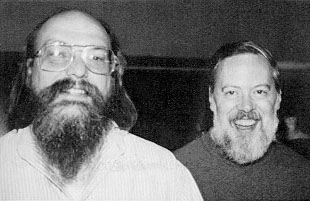
\includegraphics[width=\linewidth]{./gfx/KTDR}
	\caption%
		[Ken Thompson und Dennis Ritchie (1973) -- die Entwickler der Sprache C]
		{Ken Thompson und Dennis Ritchie (1973) -- die Entwickler der Sprache C\newline
		\url{https://en.wikipedia.org/wiki/Dennis_Ritchie}}
	\vspace{-20pt}
\end{wrapfigure}
Bis heute zählt die Sprache C zu einer der bedeutendsten Programmiersprachen. Von der Vielzahl an  Programmierpsprachen, die für verschiedenste Einsatzbereiche zur Verfügung stehen, ist ein Großteil von C beeinflusst. Ungeachtet der Existenz dieser Spezialisierungen bleibt C als Allzweck-Sprache von Bedeutung.

Es ist nicht bekannt, ob die Entwickler \emph{Dennis Ritchie} und \emph{Ken Thompson} bereits die Vision der großen Erfolge hatten, die die Sprache C einmal erreichen würde. Wie die meisten Innovationen sah auch C viele Veränderungen über die Zeit. Vermutlich der größte Erfolg ist die Tatsache, dass C bis in die jüngste Zeit hinein relevant blieb. Für die Entwickler ist es sicherlich sehr erfüllend zu sehen, dass C nicht als überholt oder als nur in Nischenanwendungen nützlich gilt. Stattdessen ist C als starke Allzweck-Sprache anerkannt.

Das Ursprüngliche Ziel der Entwickler war nicht die Entwicklung einer neuen Sprache. Tatsächlich war es erst das Zusammenspiel mehrerer Zufälle, die die Entwicklung der Sprache anstoßen. In den 1960ern arbeitete Dennis Ritchie bei Bell Labs (AT\&T) an einem Betriebssystem das von vielen Anwendern gleichzeitig benutzt werden konnte. Dieses Projekt \emph{MULTICS} (Multiplexed Information and Computer Services) sollte die gemeinsame Verwendung von Rechenressourcen erlauben. Von dem Projekt versprach man sich viele Verbesserungen -- aber bald stellte sich heraus, dass die Kosten für die Umsetzung die Vorteile überwiegen würden. Bell Labs zog sich graduell aus dem Projekt zurück.

Vor diesem Hintergrund schloss sich Ritchie dem Team von Ken Thompson und Brian Kernighan an. Thompson entwickelte in der Sprache Assembler ein Dateisystem für den DEC PDP-7 Supercomputer. Weitere Verbesserungen daran führten schließlich zur Konzeption des Betriebssystems UNIX, in dem einige der Ideen von MULTICS wieder auflebten. Tatsächlich weist schon der Originalname des neuen Projekts -- UNICS (Uniplexed Information and Computing Service) -- auf seine Verwandtschaft mit dem früheren Projekt hin.

UNIX wurde in Assembler geschrieben, was leicht für Computer umzusetzen ist, für Menschen aber eine herausfordernde Arbeitsumgebung darstellt. Um die Arbeit an UNIX zu erleichtern kamen die Sprachen Fortran und B zum Einsatz. Aus den Einschränkungen, die diese Sprachen brachten, erwuchs die Idee für die Sprache C.

Die Sprache B -- eine Weiterentwicklung der Sprache BCPL von Martin Richards -- stellte sich als nützliches Werkzeug in der Entwicklung von UNIX heraus. Jedoch mussten auch hier, wie auch in Assembler, Daten in Maschinensprache zur Verfügung gestellt werden. Datenstrukturen wurden in B ebenfalls nicht unterstützt.

Für die effiziente Fortsetzung der Arbeiten musste sich etwas ändern. Aus diesem Grunde machten sich Ritchie und seine Kollegen in den Jahren 1971 bis 73 daran, die Einschränkungen, die B ihnen auferlegte, abzuschalten. Es sollte nicht vergessen werden, dass die Sprache C im Geiste von B entwickelt wurde -- trotz oder gerade wegen dessen Beschränktheit. Viele Features und Konzepte wurden beibehalten, während neue Ideen -- darunter Datentypen und Strukturen -- hinzugefügt wurden. Der Name C weist direkt darauf hin, dass es sich hierbei um einen Nachfolger der Sprache B handelt. Anfangs wurde C im Hinblick auf die Arbeit an UNIX entwicklet. Um die Performance des Kernels und die Arbeit am Betriebssystem zu verbessern wurden viele UNIX-Komponenten neu in C umgeschrieben.

Ritchie und Kernighan dokumentierten ihr Werk in dem Buch \emph{The C Programming Language}. Obwohl Kernighan behauptete, keinen Einfluss auf das Design der Sprache C genommen zu haben, ist er doch der Autor vieler berühmter UNIX-Programme.

Bald begann C, in PCs für die Software-Entwicklung eingesetzt zu werden. Die erste (kleinere) Änderung am Sprachkonzept fand im Jahr 1983 statt, als das American National Standards Institute (ANSI) ein Kommittee zur Standardisierung der Sprache bildete. Einige Modifikationen wurden vorgenommen, die Code in der nun normierten Sprache kompatibler zu Vorgängerversionen machte. Im Jahre 1989 wurde der neue Standard verabschiedet und ist heute als ANSI C oder C89 bekannt. Die International Organization for Standardization (ISO) trug auch zur Standardisierung von C bei.

Im Laufe der Zeit hat sich C stark weiterentwickelt und Features wie Speichermanagement, Funktionen, Klassen und Bibliotheken in ihren Umfang aufgenommen und wird heute in einigen der größten und bekanntesten Projekte der Welt verwendet. Die Sprache beeinflusste die Entwicklung vieler anderer sprachen wie AMPL, AWK, csh, C++, C--, C\#, Objective-C, Bit C, D, Go, Java, JavaScript, Julia, Limbo, LPC, Perl, PHP, Pike, Processing, Python, Rust, Seed7, Vala und Verilog. 

Sind Sie ein Windows-User? Dann benutzen Sie ein Produkt, das vorwiegend in C geschrieben ist. Dasselbe gilt für MacOS, Linux, Android, iOS als auch für das Windows Phone -- kurz für alle modernen Betriebssysteme. Weiter findet C auch verbreitete Anwendung in Embedded Systems wie sie in Fahrzeugen, Smart TVs und den vielen Elementen des Internet of Things (IoT) verbaut sind.

Die vielfältigen Anwenungsfelder von C sind zu zahlreich, um sie hier aufzulisten. Einige jedoch seien als Beispiel genannt:
\begin{itemize}
\item Entwicklung von Compilern
\item Datenbanken 
\item Computer- und Handy-Spiele
\item Der UNIX-Kernel in seiner fortlaufenden Entwicklung
\item Auswertung Mathematischer Gleichungen
\item Design von Netzwerk-Geräten
\end{itemize}

Wie alle der großen Erfindungen entstand die Sprache C aus einer Notwendigkeit heraus. Die Probleme und Umstände der Zeit ihrer Entwicklung waren die Insporation für die Konzeption der Sprache. Anders als viele Sprachen, die heute als (fast) ausgestorben gelten, \enquote{gedeiht} C auch weiterhin. Einige Sprachen finden heute nur noch in Nischenbereichen Anwendung -- Fortran etwa kommt nur noch im Engineering-Bereich zum Einsatz, und COBOL hat kaum mehr Relevanz. C dagegen ist nicht nur weiterhin eine Sprache, die es zu kennen lohnt. Sie ist und bleibt Einfluss für die Weiterentwicklung bestehender und Konzeption neuer Sprachen. aufwändige Selbst Technologien wie das IoT, AI und Automations-Konzepte konnten sich nicht von der Sprache C lösen. Es bleibt zu erwarten, dass diese Sprache auch lange in die Zukunft ein Teil der Programmier-Welt bleiben wird.
\end{appendices}


	\listoffigures
\end{document}
